%\documentclass[utf8]{book}
\documentclass[10.5pt,a4paper]{ctexbook} % 五号字，A4


%========== 包 ==========
%\usepackage[UTF8]{ctex}                   % chinese
\usepackage{anyfontsize}                  % 10.5pt in ctexbook
\usepackage{booktabs}                     % \newpage
\usepackage{tcolorbox}                    % frame box
\usepackage{enumitem}                     % item
\usepackage{graphicx}                     % images
\usepackage{amsmath, amsthm, amssymb, bm} % math
\usepackage{hyperref, mathrsfs}           % ref
\usepackage{esint}                        % closed geometry integral symbol


%========== 环境 ==========
\newtheorem{definition}{定义}[section]
\newtheorem{example}{例}[section]
\newtheorem{theorem}{定理}[section]
\newtheorem{lemma}[theorem]{引理}
\newtheorem{corollary}[theorem]{推论}
\newtheorem{proposition}[theorem]{命题}


%========== enum和item设置 ==========
%\ctexset{section={beforeskip=50.0ex plus 0.2ex minus .2ex}}
%\ctexset{section={beforeskip=\doublespace}}
%\ctexset{section={format=\heiti\centering\zihao{-3},beforeskip=20cm},subsection={beforeskip=6ex}}
\ctexset{section={beforeskip=5ex},subsection={beforeskip=5ex}}
\setcounter{secnumdepth}{3}
\setcounter{tocdepth}{3}
\setenumerate[1]{itemsep=0pt,partopsep=0pt,parsep=\parskip,topsep=0pt,left=\parindent}
\setitemize[1]{itemsep=0pt,partopsep=0pt,parsep=\parskip,topsep=0pt,left=\parindent}
\setdescription{itemsep=0pt,partopsep=0pt,parsep=\parskip,topsep=5pt}
\graphicspath{{./figures}}


%========== 文档 ==========
\raggedbottom
\begin{document}


%========== 封面 ==========
\title{{\Huge{\textbf{概率论与数理统计}}}\\——学习笔记}
\author{程琰}
\date{\today}
%\linespread{1.5}
\maketitle


% %========== 前言 ==========
% \newpage
% \pagenumbering{roman}
% \setcounter{page}{1}
% \begin{center}
%     \Huge\textbf{前言}
% \end{center}

% 这是笔记的前言部分。这是笔记的前言部分。这是笔记的前言部分。这是笔记的前言部分。这是笔记的前言部分。这是笔记的前言部分。这是笔记的前言部分。

% \begin{flushright}
%     \begin{tabular}{c}
%         程琰\\
%         \today
%     \end{tabular}
% \end{flushright}


%========== 目录 ==========
\newpage
\pagenumbering{Roman}
\setcounter{page}{1}
\tableofcontents


%========== 正文 ==========
\newpage
\setcounter{page}{1}
\pagenumbering{arabic}
\chapter{随机试验与随机事件}

本章讨论概率的基础概念。
首先介绍随机和概率，再介绍两种典型概型——古典概型和几何概型，然后讨论条件对概率的影响，引出独立性和伯努利概型，最后介绍全概率模型和贝叶斯公式。

本章要点：
\begin{itemize}
    \item 事件及其基本关系，包括条件和独立。
    \item 3种基本概型：古典概型、几何概型、伯努利概型。
    \item 3个基本公式：乘法公式、全概率公式、贝叶斯公式。
\end{itemize}

\newpage
\section{试验、事件与概率}

本节介绍整个概率论中两个最基础的概念——事件和概率。

本节要点：
\begin{itemize}
    \item 掌握随机试验和随机事件的概念；
    \item 熟练掌握事件的运算法则，并熟练使用运算法则描述事件的组合；
    \item 深刻理解概率的两种定义；
    \item 熟练掌握概率计算公式，并熟练使用公式计算组合事件的概率。
\end{itemize}

%============================================================
\subsection{随机试验和随机事件}

\begin{definition}[随机试验]
若某试验满足以下三个特点：
\begin{itemize}
    \item 重复性：在相同条件下试验可重复进行；
    \item 明确性：试验的所有可能结果均事先已知；
    \item 随机性：每次试验的具体结果在试验前无法预知，
\end{itemize}
则称此试验为{\bf 随机试验}，简称{\bf 试验}，记作$E$。试验$E$的每个可能的结果称为{\bf 试验$E$的样本点}，记作$\omega $。
样本点的全体称为{\bf 试验$E$的样本空间}，记作$\varOmega $。
\end{definition}

\begin{definition}[随机事件]
我们称具有某种特征的样本点的集合为{\bf 随机事件}，简称{\bf 事件}，记作$A,B,C$等。
特别地，由一个样本点构成的单点集称为{\bf 基本事件}。任何随机事件都是样本空间$\varOmega $的子集。
若试验结果的样本点属于事件$A$，则称{\bf 事件$A$发生}，否则就称{\bf 事件$A$不发生}。
若每次试验，事件$A$必然发生，则称事件$A$为{\bf 必然事件}，显然$\varOmega $是必然事件；反之若事件$A$必然不发生，称事件$A$为{\bf 不可能事件}，显然$\oslash $是不可能事件。
\end{definition}

我们在集合论的基础上讨论随机，随机事件就是样本点的集合。

%============================================================
\subsection{事件的关系及运算法则}

事件的关系：
\begin{itemize}
    \item {\bf 包含}：若事件$A$发生必有事件$B$发生，则称事件$A$包含于事件$B$，也称事件$A$是事件$B$的子集，记作$A\subset B$。
    \item {\bf 相等}：若事件$A,B$相互包含，则称事件$A,B$相等，记作$A=B$。
    \item {\bf 并}：若事件$A,B$至少发生一个，则称事件$A,B$的并事件，记作$A\cup B$。
    \item {\bf 交}：若事件$A,B$都发生，则称事件$A,B$的交事件，记作$A\cap B$。
    \item {\bf 差}：若事件$A$发生，且事件$B$不发生，则称事件$A$和事件$B$的差事件，记作$A\cap \bar{B}$。
    \item {\bf 互斥}：若事件$A,B$不可能同时发生，则称事件$A,B$互斥，即$A\cap B=\oslash $，也称事件$A,B${\bf 互不相容}。互斥表示$A,B$没有共同样本点。
    \item {\bf 对立}：若事件$A,B$互斥，且必然发生一个，称事件$A,B$相互对立，记作$A=\bar{B}$。对立事件瓜分了整个样本空间。显然对立必互斥，而互斥并不一定对立。
\end{itemize}

\begin{figure}[h]
\centering
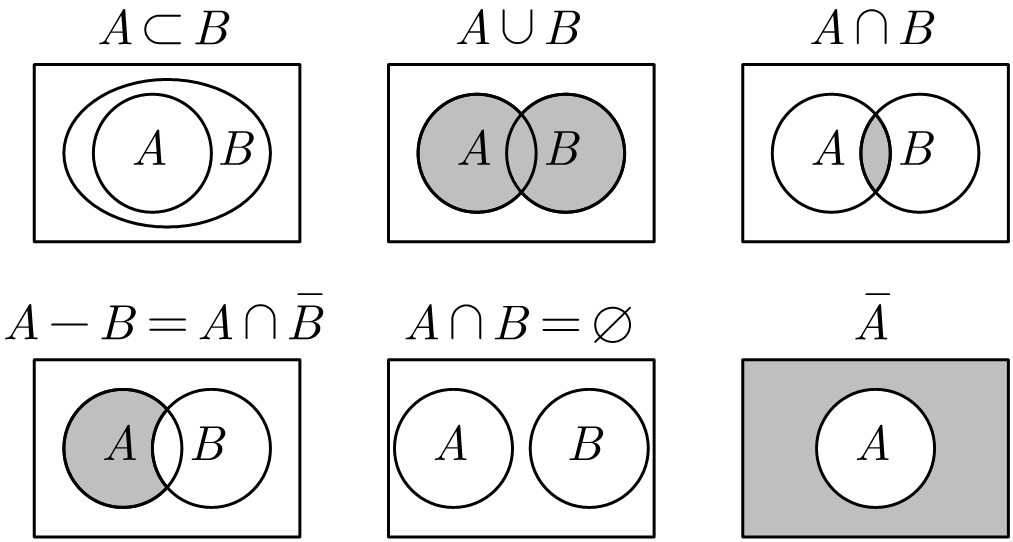
\includegraphics[height=4cm]{1.1.png}
\caption{事件的关系}
\end{figure}

事件的关系除逻辑符号外，还可使用算术符号描述：

\begin{table}[h]
\centering
\caption{事件的运算}
\begin{tabular}{ccc}
    \toprule
    运算 & 逻辑符号 & 算术符号\\
    \midrule
    并事件 & $A\cup B$ & $A+B$\\
    交事件 & $A\cap B$ & $AB$\\
    差事件 & $A\cap \bar{B}$ & $A-B$\\
    \bottomrule
\end{tabular}
\end{table}

事件的运算使得我们可以用一些简单事件的组合描述一个复杂事件。
但要注意，这里的运算是逻辑运算，而非算术运算。

\begin{tcolorbox}
为统一符号，本笔记后续$A\cup B$都记作$A+B$，$A\cap B$都记作$AB$。
\end{tcolorbox}

事件的运算法则：
\begin{itemize}
    \item {\bf 交换律}：$AB=BA$
    \item {\bf 结合律}：$\left( A+B \right) +C=A+\left( B+C \right) ,\left( AB \right) C=A\left( BC \right) $
    \item {\bf 分配律}：$\left( A+B \right) C=\left( AC \right) +\left( AB \right) ,\left( AB \right) +C=\left( A+C \right) \left( B+C \right) $
    \item {\bf 德摩根律}：$\overline{A+B}=\bar{A}\bar{B},\overline{AB}=\bar{A}+\bar{B}$
\end{itemize}

~

其他常用运算公式：
\begin{align*}
& AB\subset A\subset A+B,\qquad AB\subset B\subset A+B \\
& AA=A \\
& A+A=A \\
& A+\bar{A}=\varOmega \\
& A-B=A\bar{B}=A-AB \\
& \left( A-B \right) +B=A+B
\end{align*}


%============================================================
\subsection{概率的概念和性质}

\begin{definition}[统计定义]
将试验$E$重复$n$次，若事件$A$发生了$k$次，则称$k$为{\bf 事件$A$发生的频数}，称$\frac{k}{n}$为{\bf 事件$A$发生的频率}。
若当$n\rightarrow \infty$时，$\frac{k}{n}$有极限，则称该极限为{\bf 事件$A$的概率}，记作$P\left( A \right) $，即：
\[
P\left( A \right) := \underset{n\rightarrow \infty}{\lim}\frac{k}{n}
\]
\end{definition}

\begin{definition}[公理化定义]
设试验$E$的样本空间为$\varOmega$，对于其每个事件$A$赋予一个实数$P\left( A \right) $，若满足：
\begin{itemize}
    \item 非负性：$P\left( A \right) \geqslant 0$；
    \item 规范性：$P\left( \oslash \right) =0,P\left( \varOmega \right) =1$；
    \item 可列可加性：若事件$A_i$两两互斥，有$P\left( \bigcup_i{A_i} \right) =\sum_i{P\left( A_i \right)}$，
\end{itemize}
就称$P\left( A \right)$为{\bf 事件$A$的概率}。
\end{definition}

\begin{tcolorbox}
统计定义给出了概率的计算方法，但定义本身需要证明，具体证明在大数定理中给出。
公理化定义则不需要证明，其意义在于为一种普遍而严格的数学化概率理论奠定了基础，但缺点是没有给出具体计算方法。
还需特别注意，公理化定义中的可列可加性不是定义，而是公理！
\end{tcolorbox}

概率的性质：
\begin{itemize}
    \item {\bf 非负性}：对于任何事件$A$，有$0\leqslant P\left( A \right) \leqslant 1$；
    \item {\bf 规范性}：$P\left( \varOmega \right) =1,P\left( \oslash \right) =0$；
    \item {\bf 对立事件概率}：对于任何事件$A$，有$P\left( \bar{A} \right) =1-P\left( A \right) $；
    \item {\bf 并事件概率}：设任意事件$A,B$，有
    
    $P\left( A+B \right) =P\left( A \right) +P\left( B \right) -P\left( AB \right) $；
    \item {\bf 推论}：设任意事件$A,B,C$，有
    
    $P\left( A+B+C \right) =P\left( A \right) +P\left( B \right) +P\left( C \right) -P\left( AB \right) -P\left( AC \right) -P\left( BC \right) +P\left( ABC \right) $；
    \item {\bf 差事件概率}：设任意事件$A,B$，有$P\left( A-B \right) =P\left( A \right) -P\left( AB \right) $；
    \item {\bf 推论}：当$B\subset A$时，有$P\left( B \right) \leqslant P\left( A \right) $，且$P\left( A-B \right) =P\left( A \right) -P\left( B \right) $。
\end{itemize}

~

要点：
\begin{itemize}
    \item 我们只要记住并事件有$P\left( A+B \right) =P\left( A \right) +P\left( B \right) -P\left( AB \right) $，差事件有$P\left( A-B \right) =P\left( A \right) -P\left( AB \right) $；
    \item 特别地，若互斥$A\cap B=\oslash$，则$P\left( A+B \right) =P\left( A \right) +P\left( B \right) $；
    \item 特别地，若包含$B\subset A$，则$P\left( A-B \right) =P\left( A \right) -P\left( B \right) $。
\end{itemize}

\begin{figure}[h]
\centering
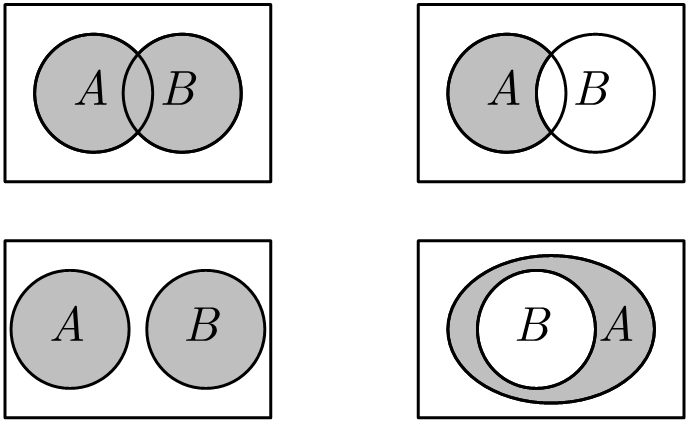
\includegraphics[height=3cm]{1.2.png}
\caption{概率的加和减}
\end{figure}

%============================================================
\subsection{概率的常用公式}

常用公式：
\begin{align*}
& P\left( \bar{A} \right) =1-P\left( A \right) \\
& P\left( A+B \right) =P\left( A \right) +P\left( B \right) -P\left( AB \right) \\
& P\left( A-B \right) =P\left( A \right) -P\left( AB \right) \\
& P\left( \bar{A}+\bar{B} \right) =P\left( \overline{AB} \right) =1-P\left( AB \right) \\
& P\left( \overline{A+B} \right) =P\left( \bar{A}\bar{B} \right) =1-P\left( A \right) -P\left( B \right) +P\left( AB \right)
\end{align*}

简单证明：
\begin{itemize}
    \item 1～3很显然，略；
    \item 4，第一个等号用德摩根律，第二个等号用公式1；
    \item 5，第一个等号用德摩根律，第二个等号考虑$P\left( \overline{A+B} \right) =1-P\left( A+B \right) $并结合公式1，略。
\end{itemize}

%============================================================
\subsection{概率的物理意义}

概率描述了事件发生的可能性的大小，若试验$E$包含了$n$个等概率的基本事件$\omega _1,\omega _2,\cdots ,\omega _n$，显然若事件$A$包含的基本事件越多，其概率越大，越容易发生。

在物理上，概率可以类比很多物理量，如物体的密度，密度越高的地方，单位体积越重，又如电荷分布，电荷密度越高的地方，电荷量越大，又如浓度，浓度越高的地方，物质含量越高。
不同的是概率在定义上是一个比值，无量纲。
对于大概率事件，我们也通常会用“大”、“多”、“集中发生”、“容易发生”等词语表述，需要根据上下文具体理解。

%============================================================
\subsection{例}

\begin{example}
设$A,B,C$为3个随机事件，用$A,B,C$表示下列事件：
\begin{enumerate}
    \item $A,B,C$中至少发生一个
    \item $A,B,C$都发生
    \item $A,B,C$中恰好发生一个
    \item $A,B,C$中至少发生两个
    \item $A$发生，且$B,C$至少一个不发生
\end{enumerate}
\end{example}

解：

\begin{enumerate}
    \item $A+B+C$
    \item $ABC$
    \item $A\bar{B}\bar{C}+\bar{A}B\bar{C}+\bar{A}\bar{B}C$
    \item $AB\bar{C}+A\bar{B}C+\bar{A}BC+ABC$
    \item $A\left( \bar{B}+\bar{C}+\bar{B}\bar{C} \right) =A\left( \bar{B}+\bar{C} \right) =A\left( \overline{BC} \right) =A-ABC$
\end{enumerate}

\begin{tcolorbox}
随机事件的相互关系，在数学上表达为集合的关系，再加之德摩根律，所以表达式并不唯一。
\end{tcolorbox}

~

\begin{example}
设$A,B$两个随机事件，已知有概率$P\left( A \right) =0.5$，$P\left( B \right) =0.4$，$P\left( A+B \right) =0.6$，计算：
\begin{enumerate}
    \item $P\left( AB \right) $
    \item $P\left( A\bar{B} \right) $
    \item $P\left( \bar{A}+\bar{B} \right) $
    \item $P\left( A+\bar{B} \right) $
\end{enumerate}
\end{example}

解：

\begin{enumerate}
    \item $\because P\left( A+B \right) =P\left( A \right) +P\left( B \right) -P\left( AB \right) \\
    \therefore P\left( AB \right) =P\left( A \right) +P\left( B \right) -P\left( A+B \right) =0.3$
    \item $P\left( A\bar{B} \right) =P\left( A-B \right) =P\left( A \right) -P\left( AB \right) =0.2$
    \item $P\left( \bar{A}+\bar{B} \right) =P\left( \overline{AB} \right) =1-P\left( AB \right) =0.7$
    \item $P\left( A+\bar{B} \right) =P\left( A \right) +P\left( \bar{B} \right) -P\left( A\bar{B} \right) =0.5+0.6-0.2=0.9$
\end{enumerate}

~

\begin{example}
设$A,B,C$三个随机事件，若$P\left( A \right) =P\left( B \right) =P\left( C \right) =\frac{1}{4}$，$P\left( AB \right) =0$，$P\left( AC \right) =P\left( BC \right) =\frac{1}{16}$，求$A,B,C$都不发生的概率。
\end{example}

解：

首先易得3个事件的德摩根律$\bar{A}\bar{B}\bar{C}=\overline{A+B+C}$，由于$P\left( AB \right) =0$则$P\left( ABC \right) =0$，于是：
\begin{align*}
&P\left( \bar{A}\bar{B}\bar{C} \right) \\
&=P\left( \overline{A+B+C} \right) =1-P\left( A+B+C \right) \\
&=1-\left[ P\left( A \right) +P\left( B \right) +P \left( C \right) -P\left( AB \right) -P\left( AC \right) -P\left( BC \right) +P\left( ABC \right) \right] \\
&=1-\left( \frac{1}{4}+\frac{1}{4}+\frac{1}{4}-\frac{1}{16}-\frac{1}{16} \right) \\
&=\frac{6}{16}
\end{align*}






\newpage
\section{古典概型和几何概型}

上节介绍了概率的定义和运算法则，但没有给出概率的计算方法。
本节介绍古典概型和几何概型及其计算方法。
古典概型是概率论的雏形，也是最简单、最常见的类型。

本节要点：
\begin{itemize}
    \item 掌握古典概型和几何概型的概念；
    \item 熟练掌握两种概型的计算方法。
\end{itemize}

%============================================================
\subsection{排列组合的概念}

\begin{definition}[排列和组合]
从$n$个元素中任取$m$个元素（$m\leqslant n$）排成一有序列，称{\bf 从$n$个元素中取出$m$个元素的一个排列}，所有排列的个数称作{\bf 排列数}，记作$P_{n}^{m}$，有：
\[
P_{n}^{m}:=\frac{n!}{\left( n-m \right) !}
\]
从$n$个元素中任取$m$个元素（$m\leqslant n$）组成一无序组，称{\bf 从$n$个元素中取出$m$个元素的一个组合}，所有组合的个数称作{\bf 组合数}，记作$C_{n}^{m}$，有：
\[
C_{n}^{m}:=\frac{n!}{\left( n-m \right) !\cdot m!}=\frac{P_{n}^{m}}{m!}
\]
特别地，$P_{n}^{1}=C_{n}^{1}=n,P_{n}^{n}=n!,C_{n}^{n}=1$。
\end{definition}

排列组合均是对“从$n$个元素中抽取$m$个元素”的计算，排列突出有序，组合突出无序。
排列组合的关系还可以这么理解，当$m$个元素排列完成后，若不考虑其顺序，就是组合，由于每个排列有$P_{m}^{m}$种不同的顺序，所以：
\[
P_{n}^{m}=C_{n}^{m}\cdot P_{m}^{m}=C_{n}^{m}\cdot m!
\]

%============================================================
\subsection{古典概型的概念}

\begin{definition}[古典概型]
若随机试验$E$满足：
\begin{itemize}
    \item 其样本空间$\varOmega $中只有有限个样本点；
    \item 每个基本事件出现的概率相等，
\end{itemize}
则称试验$E$为{\bf 古典概型试验}，或{\bf 等可能概型试验}，上述条件称为{\bf 古典概型特征}。
对于任意事件$A$，其概率$P\left( A \right) $为：
\[
P\left( A \right) :=\frac{A\text{的样本数}}{\text{总样本数}}
\]
\end{definition}

古典概型的计算基于排列组合。
在古典概型中，每个样本点具有等概率$\frac{1}{n}$，而事件就是样本点的集合，有几个样本点就是$\frac{1}{n}$的几倍。

%============================================================
\subsection{几何概型的概念}

\begin{definition}[几何概型]
若随机试验$E$满足：
\begin{itemize}
    \item 其样本空间$\varOmega $为一几何区域（一维、二维或更高任意维）；
    \item 每个基本事件出现的概率相等，
\end{itemize}
则称试验$E$为{\bf 几何概型试验}，上述条件称为{\bf 几何概型特征}。
对于任意事件$A$，其概率$P\left( A \right) $为：
\[
P\left( A \right) :=\frac{A\text{的几何测度}}{\varOmega \text{的几何测度}}
\]
\end{definition}

古典概型中样本数量是有限的，几何概型中样本数量是无限的、不可数的或是稠密的，两者分别对应离散和连续的样本空间。
通俗来讲，古典概型的计算就是“掰手指”，而几何概型就是“量尺子”。

%============================================================
\subsection{例}

\begin{example}
设有4个不同的箱子，3个不同的球，每个球可以放入任意箱子，且概率相等，计算：
\begin{enumerate}
    \item 3个球放入不同的3个箱子的概率是多少，
    \item 1号箱子和2号箱子都有球的概率是多少。
\end{enumerate}
\end{example}

解：

1. 首先计算所有可能的放置方法，每个球有4种放法，3个球共有$4^3$种放法。
然后考虑3个球放入不同的3个箱子，第一个球有4个选择，第二球剩下3个箱子选择，最后一个球只剩下2个箱子选择，所以共有$4\cdot 3\cdot 2=24$种放法，于是概率：
\[
P=\frac{4\cdot 3\cdot 2}{4^3}=\frac{3}{8}
\]

2. 1号箱子和2号箱子都有球，可分为3种情况：
\begin{itemize}
    \item 1号箱子1个球，2号箱子1个球，剩下的球在3号或4号箱子，$C_{3}^{1}\cdot C_{2}^{1}\cdot 2=12$或$P_{3}^{2}\cdot 2=12$，$P\left( A_1 \right) =\frac{12}{4^3}=\frac{12}{64}$；
    \item 1号箱子1个球，2号箱子2个球，$C_{3}^{1}\cdot C_{2}^{2}=3$，$P\left( A_2 \right) =\frac{3}{4^3}=\frac{3}{64}$；
    \item 1号箱子2个球，2号箱子1个球，$C_{3}^{2}\cdot C_{1}^{1}=3$，$P\left( A_3 \right) =\frac{3}{4^3}=\frac{3}{64}$，
\end{itemize}
且这3种情况互斥，于是：
\[
P\left( A_1+A_2+A_3 \right) =P\left( A_1 \right) +P\left( A_2 \right) +P\left( A_3 \right) =\frac{9}{32}
\]

~

\begin{example}
将一根直棒随机分成3段，求3段能构成三角形的概率。
\end{example}

解：

假设棒长$a$，3段长度分别为$x,y,\left( a-x-y \right)$，于是样本空间为：
\[
\varOmega =\{\left( x,y \right) |0<x<a,0<y<a,a-x-y>0\}
\]
在{\it xy}平面上为{\it x}轴、{\it y}轴和直线$y=a-x$构成的面积。
能构成三角的充要条件是任意两边之和大于第三边，于是：
\[
\begin{cases}
	x+y>a-x-y\\
	x+\left( a-x-y \right) >y\\
	y+\left( a-x-y \right) >x\\
\end{cases}\qquad \Rightarrow \qquad \begin{cases}
	x+y>\frac{a}{2}\\
	y<\frac{a}{2}\\
	x<\frac{a}{2}\\
\end{cases}
\]
在\textit{xy}平面上为3条直线$x=\frac{a}{2}$、$y=\frac{a}{2}$和$y=\frac{a}{2}-x$构成的面积，可得概率为$1/4$。

\begin{figure}[h]
\centering
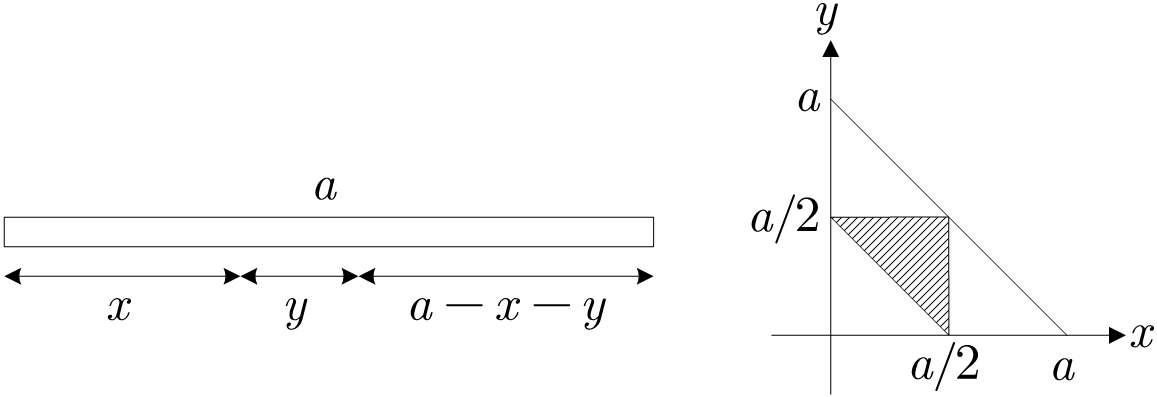
\includegraphics[height=3cm]{1.3.png}
\end{figure}






\newpage
\section{条件概率}

\begin{tcolorbox}
现实中，我们有时知道某个事件$A$发生了，此时，试验的部分不确定因素变成了确定性因素，在这种情况下，需要计算事件$B$的概率，这就是条件概率。
\end{tcolorbox}

本节介绍条件概率，也是后续全概率公式、贝叶斯公式、事件独立性的基础。

本节要点：
\begin{itemize}
    \item 掌握条件概率的概念、性质和公式；
    \item 掌握独立性的概念；
    \item 深刻理解伯努利概型。
\end{itemize}

%============================================================
\subsection{条件概率的概念和性质}

\begin{definition}[条件概率]
在事件$A$发生的情况下，事件$B$发生的概率称为{\bf 条件概率}，记作$P\left( B \middle| A \right) $，当$P\left( A \right) >0$时有：
\[
P\left( B \middle| A \right) := \frac{P\left( AB \right)}{P\left( A \right)}
\]
\end{definition}

$P\left( B \middle| A \right) $和$P\left( B \right) $的大小关系是不定的。
也就是说，事件$A$的发生并不一定有利于$B$，也可能没有影响。
切不能想当然地认为$P\left( B \middle| A \right) >P\left( B \right) $！

从原理上来讲，一切概率都是必然事件的条件概率，这种必然事件可以理解为试验所规定的基本条件。
但在一般性的讨论中，条件指的是除了基本条件之外的额外的条件。

~

条件概率的性质：
\begin{itemize}
    \item {\bf 非负性}：$0\leqslant P\left( B \middle| A \right) \leqslant 0$；
    \item {\bf 规范性}：$P\left( \varOmega \middle| A \right) =1,P\left( \oslash \middle| A \right) =0$；
    \item {\bf 对立事件概率}：对于任何事件$B$，有$P\left( \bar{B} \middle| A \right) =1-P\left( B \middle| A \right) $；
    \item {\bf 并事件概率}：设任意事件$A,B$，有
    
    $P\left[ \left( B_1+B_2 \right) \middle| A \right] =P\left( B_1 \middle| A \right) +P\left( B_2 \middle| A \right) -P\left( B_1B_2 \middle| A \right) $
    \item {\bf 差事件概率}：设任意事件$B_1,B_2$，有
    
    $P\left[ \left( B_1-B_2 \right) \middle| A \right] =P\left( B_1 \middle| A \right) -P\left( B_1B_2 \middle| A \right) $；
    \item {\bf 有限可加性}：若事件$B_i$两两互斥，则有$P\left( \bigcup_i{B_i} \middle| A \right) =\sum_i{P\left( B_i \middle| A \right)}$。
\end{itemize}

~

对比单个概率的性质，有一样的要点：
\begin{itemize}
    \item 我们只要记住并事件有
    
    $P\left[ \left( B_1+B_2 \right) \middle| A \right] =P\left( B_1 \middle| A \right) +P\left( B_2 \middle| A \right) -P\left( B_1B_2 \middle| A \right) $，
    
    差事件有
    
    $P\left[ \left( B_1-B_2 \right) \middle| A \right] =P\left( B_1 \middle| A \right) -P\left( B_1B_2 \middle| A \right) $；
    \item 特别地，若互斥$B_2\cap B_1=\oslash$，则并事件有
    
    $P\left[ \left( B_1+B_2 \right) \middle| A \right] =P\left( B_1 \middle| A \right) +P\left( B_2 \middle| A \right) $；
    \item 特别地，若包含$B_2\subset B_1$，则差事件有
    
    $P\left[ \left( B_1-B_2 \right) \middle| A \right] =P\left( B_1 \middle| A \right) -P\left( B_2 \middle| A \right) $。
\end{itemize}


%============================================================
\subsection{条件概率的乘法公式}

\begin{theorem}[乘法公式]
若$P\left( A \right) >0$，则
\[
P\left( AB \right) =P\left( A \right) \left( B \middle| A \right)
\]
\end{theorem}

\begin{corollary}[乘法公式]
若$P\left( A_1A_2\cdots A_n \right) >0,n\geqslant 2$，则
\[
P\left( A_1A_2\cdots A_n \right) =P\left( A_1 \right) P\left( A_2 \middle| A_1 \right) P\left( A_3 \middle| A_1A_2 \right) \cdots P\left( A_n \middle| A_1A_2\cdots A_{n-1} \right)
\]
\end{corollary}


%============================================================
\subsection{独立性的概念}

\begin{tcolorbox}
本节开始就提到，事件$A$的发生并不一定有利于事件$B$，也可能没有影响。
这种“没影响”就是下面定义的独立性。
反映到表达式就是$P\left( B \right) =P\left( B \middle| A \right) =P\left( B \middle| \bar{A} \right) $。
\end{tcolorbox}

\begin{definition}[独立性]
设事件$A,B$，若$P\left( AB \right) =P\left( A \right) P\left( B \right) $，则称{\bf 事件$A,B$相互独立}。
该定义也可扩展到3个事件，若$P\left( ABC \right) =P\left( A \right) P\left( B \right) P\left( C \right) $，称{\bf 事件$A,B,C$相互独立}。
甚至多个事件，略。
注意，若$A,B,C$相互独立，则任意两个事件必然相互独立，常称为{\bf 两两独立}，但两两独立并不一定相互独立。
\end{definition}

\begin{theorem}
~
\begin{itemize}
    \item 若事件$A,B$相互独立，则$P\left( AB \right) =P\left( A \right) P\left( B \right) $。
    \item 若$P\left( A \right) \ne 0$，则有，事件$A,B$相互独立$\Leftrightarrow P\left( B \middle| A \right) =P\left( B \right) $。
    \item 若$0<P\left( A \right) <1$，则有，事件$A,B$相互独立$\Leftrightarrow P\left( B \middle| A \right) =P\left( B \middle| \bar{A} \right) $。
    \item 若$A,B$相互独立，则$\bar{A},B$相互独立、$A,\bar{B}$相互独立、$\bar{A},\bar{B}$相互独立，任意反之依然，即这4个命题相互等价。
    \item 若$A_1,A_2,\cdots ,A_n$相互独立，则任意抽取若干个事件也相互独立。
    \item 若$A_1,A_2,\cdots ,A_n$相互独立，则将某个事件取反$\bar{A}_i$组成的事件组也相互独立。
    \item 若$A_1,A_2,\cdots ,A_n$相互独立，则将它们任意分成两组，这两组事件相互独立。
\end{itemize}
\end{theorem}

我们从条件概率考察独立性，由于条件概率$P\left( B \middle| A \right) =\frac{P\left( AB \right)}{P\left( A \right)}$总是成立的，所以$P\left( AB \right) =P\left( A \right) P\left( B \right) $反映了$P\left( B \middle| A \right) =P\left( B \right) $，即事件$A$的发生与否对事件$B$没有影响。
其次，我们一般不从定义判断两个事件是否独立，而是从事件的事实角度判断，如果两个事件独立，则采用第一条定理的公式计算。
通常而言，如果事件$A$描述了试验$E_A$的结果，事件$B$描述了试验$E_B$的结果，试验$E$由$E_A,E_B$构成，且$E_A,E_B$不存在相互逻辑关系，则$A,B$相互独立。

%============================================================
\subsection{关于互斥和独立}

互斥关注事件的样本点，表示两个事件没有公共样本点。
独立关注事件的概率，表示两个事件有各自的试验背景，互不影响。

以掷骰子为例，将1颗骰子投掷2次，分别记录第一次和第二次的点数，将$\left( i,j\right) $记作样本点。

若设2个事件：
\begin{align*}
& A=\left\{ \left( 1,1 \right) ,\left( 2,2 \right) ,\left( 3,3 \right) \right\} \\
& B=\left\{ \left( 4,4 \right) ,\left( 5,5 \right) ,\left( 6,6 \right) \right\}
\end{align*}
则$A,B$互斥，它们之间没有任何公共样本点，而且$P\left( AB \right) =0$，所以$P\left( B \middle| A \right) =0$。

若：
\begin{align*}
& A=\left\{ \text{其中一次点数为}5 \right\} \\
& B=\left\{ \text{两次点数之和为偶数} \right\}
\end{align*}
显然$A,B$不互斥，比方它们均有有样本点$\left( 5,3 \right) $，而且$A,B$通过第一颗骰子的点数有了关系，所以$A,B$不独立。

再若：
\begin{align*}
& A=\left\{ \text{第一次点数为}5 \right\} \\
& B=\left\{ \text{第二次点数为}4 \right\}
\end{align*}
虽然$A,B$有公共样本点$\left( 5,4 \right) $，但$A,B$分属于两个不搭界的小试验，所以$A,B$独立。

%============================================================
\subsection{伯努利概型}

\begin{definition}[伯努利试验]
设试验$E$是由重复$n$次的一系列子试验$E_i,i=1,2,\cdots ,n$组成，若：
\begin{itemize}
    \item 每次子试验$E_i$对应的样本空间相同；
    \item 每次子试验$E_i$的结果相互独立，
\end{itemize}
则称该试验$E$为{\bf $n$重独立重复试验}。
进一步，如果每次子试验$E_i$只考虑事件$A,\bar{A}$，则称试验$E$为{\bf $n$重伯努利试验}。
\end{definition}

\begin{theorem}
在$n$重伯努利试验$E$中，事件$A$恰好发生$k$次的概率为：
\[
C_{n}^{k}p^k\left( 1-p \right) ^{n-k}
\]
其中：
\begin{itemize}
    \item $p=P\left( A \right) $：事件$A$在每次子试验$E_i$中发生的概率；
    \item $C_{n}^{k}$：$n$次子试验中，事件$A$发生了$k$次，注意，这里用组合，表示我们只关心$k$次，而不关心具体是哪$k$次；
    \item $p^k$：事件$A$发生$k$次的概率；
    \item $\left( 1-p \right) ^{n-k}$：其余$n-k$次子试验中事件$A$不发生的概率。
\end{itemize}
\end{theorem}

伯努利试验是一个等概率二元重复试验，有3个要点：
\begin{itemize}
    \item 首先，是一个重复性试验，即试验$E$由一系列子试验组成；
    \item 其次，每个子试验只考虑事件$A$的发生和不发生；
    \item 最后，事件$A$在每次子试验中的概率$P\left( A\right) $保持一致。
\end{itemize}
对于试验结果，我们只关心事件$A$发生$k$次的概率，而不考虑具体是哪$k$次发生。

%============================================================
\subsection{例}

\begin{example}
设10件产品中有4件次品，从中任意抽取2件，若其中一件为次品，计算另一件也为次品的概率。
\end{example}

解：

记其中一件为次品为事件$A$，再记两件均为次品为事件$AB$，题干要求的概率可以表示为条件概率$P\left( B \middle| A \right) =\frac{P\left( AB \right)}{P\left( A \right)}$，于是：
\begin{align*}
& \because \begin{cases}
	P\left( A \right) =1-P\left( \bar{A} \right) =1-\frac{C_{6}^{2}}{C_{10}^{2}}=\frac{30}{45}\\
	P\left( AB \right) =\frac{C_{4}^{2}}{C_{10}^{2}}=\frac{6}{45}\\
\end{cases}
\\
& \therefore P\left( B \middle| A \right) =\frac{P\left( AB \right)}{P\left( A \right)}=\frac{1}{5}
\end{align*}

~

\begin{example}
同上产品，任取2件，若第一次抽取到为次品，计算此时第二次也为次品的概率。
\end{example}

解：

从事实出发，第一次抽取到次品后情况变成9件产品，其中3件为次品，抽取到次品的概率自然为$3/9=1/3$。

~

\begin{example}
设有50个晶体管中有2个次品，每次任取1个，且不放回，求：
\begin{enumerate}
    \item 第4次取到最后一个次品的概率，
    \item 至少抽取几个才能使出现次品的概率超过0.6。
\end{enumerate}
\end{example}

解：

1. 记第$i$次取到次品的概率为$P\left( A_i \right) $，则第4次取到最后一个次品可分为3种情况，分别为第1次取到次品、第2次取到次品、第3次取到次品，且这3种情况互不相容，于是：
\begin{align*}
&P\left( A_1\bar{A}_2\bar{A}_3A_4+\bar{A}_1A_2\bar{A}_3A_4+\bar{A}_1\bar{A}_2A_3A_4 \right) \\
&=P\left( A_1\bar{A}_2\bar{A}_3A_4 \right) +P\left( \bar{A}_1A_2\bar{A}_3A_4 \right) +P\left( \bar{A}_1\bar{A}_2A_3A_4 \right)
\end{align*}
直接计算较为复杂，可利用乘法公式：
\begin{align*}
&\begin{aligned}
	P\left( A_1\bar{A}_2\bar{A}_3A_4 \right) &=P\left( A_1 \right) P\left( \bar{A}_2 \middle| A_1 \right) P\left( \bar{A}_3 \middle| A_1\bar{A}_2 \right) P\left( A_4 \middle| A_1\bar{A}_2\bar{A}_3 \right)\\
	&=\frac{2}{50}\cdot \frac{48}{49}\cdot \frac{47}{48}\cdot \frac{1}{47}=\frac{1}{1225}\\
	P\left( \bar{A}_1A_2\bar{A}_3A_4 \right) &=P\left( \bar{A}_1 \right) P\left( A_2 \middle| \bar{A}_1 \right) P\left( \bar{A}_3 \middle| \bar{A}_1A_2 \right) P\left( A_4 \middle| \bar{A}_1A_2\bar{A}_3 \right)\\
	&=\frac{48}{50}\cdot \frac{2}{49}\cdot \frac{47}{48}\cdot \frac{1}{47}=\frac{1}{1225}\\
	P\left( \bar{A}_1\bar{A}_2A_3A_4 \right) &=P\left( \bar{A}_1 \right) P\left( \bar{A}_2 \middle| \bar{A}_1 \right) P\left( A_3 \middle| \bar{A}_1\bar{A}_2 \right) P\left( A_4 \middle| \bar{A}_1\bar{A}_2A_3 \right)\\
	&=\frac{48}{50}\cdot \frac{47}{49}\cdot \frac{2}{48}\cdot \frac{1}{47}=\frac{1}{1225}\\
\end{aligned} \\
&P=\frac{3}{1225}
\end{align*}

2. 设连续抽取$n$个均为正品，则概率可记为$P\left( \bar{A}_1\bar{A}_2\cdots \bar{A}_n \right) $，利用乘法公式：
\begin{align*}
&P\left( \bar{A}_1\bar{A}_2\cdots \bar{A}_n \right) =P\left( \bar{A}_1 \right) P\left( \bar{A}_2 \middle| \bar{A}_1 \right) \cdots P\left( \bar{A}_n \middle| \bar{A}_1\bar{A}_2\bar{A}_3\cdots \bar{A}_{n-1} \right) \\
&=\frac{48}{50}\cdot \frac{47}{49}\cdot \frac{46}{48}\cdot \frac{45}{47}\cdots \frac{48-\left( n-3 \right)}{50-\left( n-3 \right)}\cdot \frac{48-\left( n-2 \right)}{50-\left( n-2 \right)}\cdot \frac{48-\left( n-1 \right)}{50-\left( n-1 \right)} \\
&=\frac{48}{50}\cdot \frac{47}{49}\cdot \frac{46}{48}\cdot \frac{45}{47}\cdots \frac{51-n}{53-n}\cdot \frac{50-n}{52-n}\cdot \frac{49-n}{51-n} \\
&=\frac{\left( 50-n \right) \cdot \left( 49-n \right)}{50\cdot 49}
\end{align*}
则在抽取的$n$个样品中，出现次品的概率为：
\[
1-P\left( \bar{A}_1\bar{A}_2\cdots \bar{A}_n \right) =1-\frac{\left( 50-n \right) \cdot \left( 49-n \right)}{50\cdot 49}=\frac{99n-n^2}{50\cdot 49}
\]
计算$\frac{99n-n^2}{50\cdot 49}>0.6$可得：
\begin{align*}
&\because \frac{99n-n^2}{50\cdot 49}>0.6 \Rightarrow n^2-99n+1470<0 \\
&\therefore n^2-99n+1470=0 \Rightarrow n=\frac{99\pm \sqrt{99^2-4\cdot 1470}}{2}=80.8 \mathrm{or} 18.2 \\
&\therefore n<80.8 \quad \mathrm{or} \quad n>18.2
\end{align*}
可以当抽取19个及以上时，出现次品的概率大于0.6。
注意，这里不是说抽到第19个才出现次品，而是19个中必有次品。

~

\begin{example}
将一枚硬币反复抛5次，求至少2次正面向上的概率。
\end{example}

解：

这是典型的伯努利概型，可利用公式$C_{n}^{k}p^k\left( 1-p \right) ^{n-k}$计算0次正面向上和1次正面向上后“取反”，以减小计算量：
\begin{align*}
P&=1-\sum_{k=0}^1{C_{5}^{k}\left( \frac{1}{2} \right) ^k\left( 1-\frac{1}{2} \right) ^{5-k}} \\
&=1-C_{5}^{0}\left( \frac{1}{2} \right) ^0\left( 1-\frac{1}{2} \right) ^{5-0}-C_{5}^{1}\left( \frac{1}{2} \right) ^1\left( 1-\frac{1}{2} \right) ^{5-1} \\
&=\frac{13}{16}
\end{align*}
也可用$P=\sum_{k=2}^5{C_{5}^{k}\left( \frac{1}{2} \right) ^k\left( 1-\frac{1}{2} \right) ^{5-k}}$，但计算量较大。

~

\begin{example}
假设事件$A$的发生概率小于0.5，若在4重伯努利试验中， 恰好发生2次的概率为$8/27$，求在4重伯努利试验中， 恰好发生1次的概率。
\end{example}

解：

设事件$A$的发生概率为$p$，由题干可得：
\begin{align*}
&\because C_{4}^{2}p^2\left( 1-p \right) ^{4-2}=\frac{4!}{2!\cdot 2!}p^2\left( 1-p \right) ^2=\frac{8}{27} \\
&\therefore p\left( 1-p \right) =\frac{2}{9} \\
&\therefore p=\frac{1}{3}\mathrm{or} \frac{2}{3}
\end{align*}
由于事件$A$的发生概率小于0.5，所以取$p=1/3$。
于是在4重伯努利试验中，$A$恰好发生1次的概率：
\[
C_{4}^{1}p^1\left( 1-p \right) ^{4-1}=\frac{4!}{3!\cdot 1!}\cdot \frac{1}{3}\cdot \left( \frac{2}{3} \right) ^3=\frac{32}{81}
\]






\newpage
\section{全概率公式与贝叶斯公式}

本节介绍全概率公式和贝叶斯公式。

本节要点：
\begin{itemize}
    \item 掌握全概率公式；
    \item 掌握贝叶斯公式；
    \item 了解先验概率和后验概率的关系。
\end{itemize}

%============================================================
\subsection{完备事件组和全概率公式}

\begin{definition}[完备事件组]
若事件组$A_1,A_2,\cdots ,A_i,\cdots $两两互斥，且$A_1+A_2+\cdots +A_i+\cdots =\varOmega $，则$A_1,A_2,\cdots ,A_i,\cdots $构成样本空间 的一个{\bf 完备事件组}，简称{\bf 完备组}。
\end{definition}

\begin{definition}[全概率公式]
若事件组$A_1,A_2,\cdots ,A_i,\cdots $构成样本空间$\varOmega $的一个完备组，则对于任何事件$B$有：
\[
P\left( B \right) =\sum_{i=1}^{\infty}{P\left( A_iB \right)}=\sum_{i=1}^{\infty}{\left[ P\left( A_i \right) \cdot P\left( B \middle| A_i \right) \right]}
\]
\end{definition}

\begin{figure}[h]
\centering
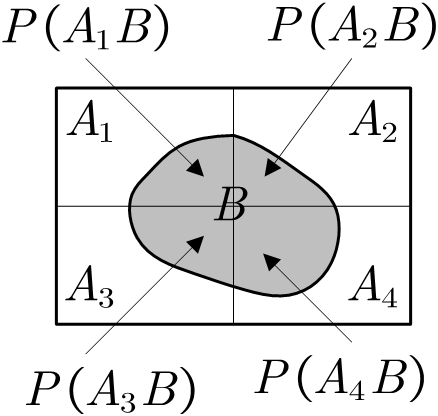
\includegraphics[height=3cm]{1.4.png}
\caption{全概率}
\end{figure}

完备组“瓜分”了整个样本空间，是事件对立关系的扩充，其意义在于将一个复杂的大问题分解为若干个简单的小问题。

全概率可以认为是条件概率的延申，如果事件组满足完备条件，则事件$B$的发生总是伴随某个组员的发生，或者说$B$是通过某个路径发生的。
当$P\left( B \right) $的计算较为复杂时，我们可以构造一个合适的完备组，简化$P\left( B \right) $的计算。
其次，该公式从数学上还可以理解为$P\left( B \right) $是$P\left( B \middle| A_i \right) $的加权和，权重为$P\left( A_i \right) $。
最后还需注意，$P\left( B \right) \leqslant 1$，但$\sum_{i=1}^{\infty}{P\left( B \middle| A_i \right)}$几乎可能大于1。

%============================================================
\subsection{贝叶斯公式}

\begin{definition}[贝叶斯公式]
若事件$A_1,A_2,\cdots ,A_i,\cdots $构成样本空间$\varOmega $的一个完备事件组，且$P\left( A_i \right) >0$，若$B$为一随机事件，且$P\left( B \right) >0$，则：
\[
P\left( A_i \middle| B \right) =\frac{P\left( A_i \right) P\left( B \middle| A_i \right)}{\sum_{i=1}^{\infty}{\left[ P\left( A_i \right) \cdot P\left( B \middle| A_i \right) \right]}}=\frac{P\left( A_i \right) P\left( B \middle| A_i \right)}{P\left( B \right)}
\]
又称{\bf 逆概率公式}。
通常，我们将$P\left( A_i \right) $称为{\bf 先验概率}，将条件概率$P\left( A_i \middle| B \right) $称为{\bf 后验概率}。
\end{definition}

\begin{proof}
由条件概率的概念可得：
\[
P\left( A_i \middle| B \right) =\frac{P\left( A_iB \right)}{P\left( B \right)}
\]
结合全概率公式，且$P\left( A_iB \right) =P\left( BA_i \right) =P\left( A_i \right) P\left( B \middle| A_i \right) $。
\end{proof}

$P\left( A_i \right) $称为先验概率的原因是$A_i$作为一种假定而不依赖于$B$。
$B$称为{\bf 证据}，一种出现的客观事物。
在证据出现前，$A_i$有自己的概率。
当证据发现时，$A_i$的概率变成了$P\left( A_i \middle| B \right) $，所以我们称为后验概率。
“先”和“后”指的是证据出现前和出现后。
其中$P\left( B \middle| A_i \right) $描述了$A_i$和$B$的关系，机器学习中称为{\bf 似然（likehood）}。

如下图，$P\left( A_1 \right) =P\left( A_2 \right) =P\left( A_3 \right) =P\left( A_4 \right) =1/4$，但如果$B$发生了，显然有利于$A_1$的发生且$P\left( A_1 \right) >1/4$，不利于$A_4$的发生且$P\left( A_4 \right) <1/4$。
\begin{figure}[h]
\centering
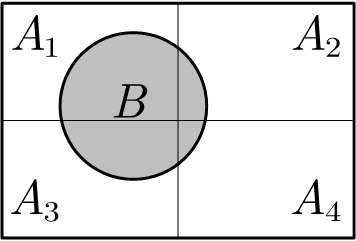
\includegraphics[height=2cm]{1.5.png}
\end{figure}

全概率公式体现了由因求果，而贝叶斯公式反映了执果寻因的一种辩证思想，我们知道完备组员的概率$P\left( A_i \right) $和$B$在各个完备组员的条件概率$P\left( B \middle| A_i \right) $，就可以计算$B$大概会发生在哪个组员。
很多情况下，我们知道各个原因发生的可能性，但是一旦结果出现，这些原因的可能性又会出现变化，贝叶斯公式揭示了两者之间的关系。

%============================================================
\subsection{例}

\begin{example}
设10件产品中存在2件次品，现不放回地抽取2次，每次1件，求第2件是次品的概率。
\end{example}

解：

由题干可知，第2件是否为次品的概率和第1件为否是次品有关，所以这是典型的条件概率。
更进一步，第1件产品的合格和次品两个事件可以构成完备组，所以可以用全概率公式求解。

设第1次抽取为次品为事件$A$，于是$A,\bar{A}$可视为完备组，且易得$P\left( A \right) =\frac{2}{10},P\left( \bar{A} \right) =\frac{8}{10}$。
再设第2次抽到次品为事件$B$，于是$P\left( B \right) $可以用这个完备组分解：
\[
P\left( B \right) =P\left( A \right) P\left( B \middle| A \right) +P\left( \bar{A} \right) P\left( B \middle| \bar{A} \right)
\]
其中：
\begin{itemize}
    \item $P\left( B \middle| A \right) $：表示第1次抽到次品时第2次也抽到次品的概率，易得$\frac{1}{9}$；
    \item $P\left( B \middle| \bar{A} \right) $：表示第1次抽到合格时第2次抽到次品的概率，易得$\frac{2}{9}$。
\end{itemize}
最终得到：
\[
P\left( B \right) =\frac{1}{5}\cdot \frac{1}{9}+\frac{4}{5}\cdot \frac{2}{9}=\frac{1}{5}
\]

解二，不用全概率的概念，直接使用古典概型的方法，抽取2件排序，共$P_{10}^{2}$种，第2件是次品有两种互不相同可能：
\begin{itemize}
    \item 第1次抽到次品时第2次也抽到次品，$C_{2}^{1}\cdot C_{1}^{1}$种；
    \item 第1次抽到合格时第2次抽到次品，$C_{8}^{1}\cdot C_{2}^{1}$种。
\end{itemize}
于是：
\[
P=\frac{C_{2}^{1}\cdot C_{1}^{1}+C_{8}^{1}\cdot C_{2}^{1}}{P_{10}^{2}}=\frac{18}{90}=\frac{1}{5}
\]

~

\begin{example}
假设血清甲蛋白法测定肝癌阳性准确率为95\%、阴性准确率为90\%，若已知社会人群的患癌率为0.04\%，若某人检测阳性，分析其实际患癌的概率。
\end{example}

解：

设事件$A$表示被检者实际患癌，事件$B$ 表示用该测定法判定阳性，由题干可知：
\begin{align*}
&P\left( A \right) =0.0004 \\
&P\left( B \middle| A \right) =0.95 \\
&P\left( \bar{B} \middle| \bar{A} \right) =0.90
\end{align*}
由于$A,\bar{A}$构成完备组，则有：
\begin{align*}
P\left( A \middle| B \right) &=\frac{P\left( A \right) P\left( B \middle| A \right)}{P\left( A \right) P\left( B \middle| A \right) +P\left( \bar{A} \right) P\left( B \middle| \bar{A} \right)} \\
&=\frac{0.0004\cdot 0.95}{0.0004\cdot 0.95+0.9996\cdot \left( 1-0.9 \right)} =0.00378712
\end{align*}

一方面可见即便测定阳性，实际患癌也不到1\%，但比一般人群已经高了$0.3787/0.04=9.4675$，将近10倍。
另一方面，通过贝叶斯公式我们了解到，血清甲蛋白测定法不是判断患癌的概率，而是判断比正常人患癌概率高了多少。

\begin{tcolorbox}
该例子很具典型性。
首先0.04\%的患癌概率是作为一种先天的经验存在。
测试结果则是一种证据。
证据的出现可以让我们对这个先天经验进行修正。
由于这个证据本身带有概率，而非100\%，所以它实际上是提高了患癌概率。
\end{tcolorbox}

~

\begin{example}
某水文站测量水流量，令$B$为测量不准的事件，并总结了几个测量不准的原因$A_i$，原因的发生概率$P\left( A_i \right) $，以及某个原因发生时测量不准的概率$P\left( B \middle| A_i \right) $，如下表，分析哪几个原因主要导致了测量不准。
\begin{table}[h]
\centering
\begin{tabular}{ccc}
    \toprule
    测不准的原因$A_i$ & $P\left( A_i \right) $ & $P\left( B \middle| A_i \right) $\\
    \midrule
    流速计故障 & 0.01 & 0.90\\
    绕道设备误差 & 0.05 & 0.80\\
    水中有杂质 & 0.04 & 0.10\\
    气象条件不佳 & 0.10 & 0.30\\
    人员配合问题 & 0.10 & 0.80\\
    其他 & 0.70 & 0.01\\
    \bottomrule
\end{tabular}
\end{table}
\end{example}

解：

“那几个原因主要导致了测量不准”也即测量不准的情况下，各个原因的发生概率$P\left( A_i \middle| B \right) $，可以用贝叶斯公式解决。
\[
P\left( A_i \middle| B \right) =\frac{P\left( A_i \right) P\left( B \middle| A_i \right)}{P\left( B \right)}=\frac{P\left( A_i \right) P\left( B \middle| A_i \right)}{\sum_{i=1}^{\infty}{P\left( A_i \right) P\left( B \middle| A_i \right)}}
\]
计算结果如下表。
可见，单看每个已知的明确的原因，它们的发生概率都不大，但是一旦问题出现，最有可能是人员配合导致。
所以若要提高测量准确度，首先得从提高人员配合度着手。
\begin{table}[ht]
    \centering
    \begin{tabular}{cccc}
        \toprule
        测不准的原因$A_i$ & $P\left( A_i \right) $ & $P\left( B \middle| A_i \right) $ & $P\left( A_i \middle| B \right) $\\
        \midrule
        流速计故障 & 0.01 & 0.90 & 0.05\\
        绕道设备误差 & 0.05 & 0.80 & 0.24\\
        水中有杂质 & 0.04 & 0.10 & 0.02\\
        气象条件不佳 & 0.10 & 0.30 & 0.18\\
        人员配合问题 & 0.10 & 0.80 & 0.47\\
        其他 & 0.70 & 0.01 & 0.04\\
        \bottomrule
    \end{tabular}
\end{table}

~

\begin{example}
甲箱中有2个白球4个黑球，乙箱中有6个白球2个黑球，现从这两箱中各任取一球，再从所取出的两球中任取一球，求最终该球是白球的概率。
\end{example}

解：

令从甲箱中取得白球为事件$A$，从乙箱中取得白球为事件$B$，易得甲乙两个箱子中取球为独立事件，于是：
\begin{align*}
&P\left( A \right) =\frac{1}{3},P\left( B \right) =\frac{3}{4} \\
&P\left( AB \right) =\frac{1}{4},P\left( A\bar{B} \right) =\frac{1}{12},P\left( \bar{A}B \right) =\frac{1}{2},P\left( \bar{A}\bar{B} \right) =\frac{1}{6}
\end{align*}
且$AB,\bar{A}B,A\bar{B},\bar{A}\bar{B}$构成完备组，于是可以用全概率公式得到：
\begin{align*}
P\left( C \right) =&P\left( AB \right) P\left( C \middle| AB \right) +P\left( A\bar{B} \right) P\left( C \middle| A\bar{B} \right) + \\
&P\left( \bar{A}B \right) P\left( C \middle| \bar{A}B \right) +P\left( \bar{A}\bar{B} \right) P\left( C \middle| \bar{A}\bar{B} \right)
\end{align*}
而易得：
\begin{align*}
&P\left( C \middle| AB \right) =1 \\
&P\left( C \middle| A\bar{B} \right) =P\left( C \middle| \bar{A}B \right) =\frac{1}{2} \\
&P\left( C \middle| \bar{A}\bar{B} \right) =0
\end{align*}
于是：
\[
P\left( C \right) =\frac{1}{4}+\frac{1}{12}\cdot \frac{1}{2}+\frac{1}{2}\cdot \frac{1}{2}=\frac{13}{24}
\]






\newpage
\section{从线性代数理解本章概念}

本节从线性代数的角度考察本章的几个概念，以加深对这些概念的理解。

%============================================================
\subsection{完备组和规范正交基}

完备组可以认为是样本空间的一组基，为方便讨论，假设完备组有限个，记作
\[
A=\left\{ P\left( A_1 \right) ,P\left( A_2 \right) ,\cdots ,P\left( A_n \right) \right\}
\]
其中：
\begin{itemize}
    \item $A$：基；
    \item $P\left( A_i \right) $：$A_i$的坐标。
\end{itemize}
且这个完备组具备以下特征：
\begin{itemize}
    \item 由于$\sum_{i=1}^n{P\left( A_i \right)}=1$，所以可以认为该组基是规范的；
    \item $A_i$由于互斥，所以可以认为该组基是正交的；
    \item 更进一步，如果$P\left( A_1 \right) =P\left( A_2 \right) =\cdots =P\left( A_n \right) $，可以认为该组基是标准基。
\end{itemize}


%============================================================
\subsection{全概率和坐标}

全概率公式$P\left( B \right) =\sum_{i=1}^n{\left[ P\left( A_i \right) \cdot P\left( B \middle| A_i \right) \right]} $中，$P\left( B \middle| A_i \right) $可以认为是事件$B$在基$A_i$下的坐标分量，该分量越大，表示越可能发生。
用线性代数的方式可以记作
\[
P\left( B \right) =\left[ \begin{matrix}
	P\left( A_1 \right)&		P\left( A_2 \right)&		\cdots&		P\left( A_n \right)\\
\end{matrix} \right] \left[ \begin{array}{c}
	P\left( B \middle| A_1 \right)\\
	P\left( B \middle| A_2 \right)\\
	\cdots\\
	P\left( B \middle| A_n \right)\\
\end{array} \right] =A\left[ B \right] _A
\]
其中：
\begin{itemize}
    \item $\left[ B \right] _A=\left( \begin{matrix} P\left( B \middle| A_1 \right)&		P\left( B \middle| A_2 \right)&		\cdots&		P\left( B \middle| A_n \right) \end{matrix} \right) ^T$：向量$B$（也即事件$B$）在基$A$下的坐标向量。
\end{itemize}

这里与线性代数不一样，基$A$的表达并不是一个矩阵，而是一个向量，所以事件$B$在样本空间的坐标$P\left( B \right) $是一个标量。

%============================================================
\subsection{再论贝叶斯公式}

由于$B,\bar{B}$也可以构成一个完备组，也是一组规范正交基。
所以$P\left( A_i \middle| B \right) $表达的是基$A$中的$A_i$在基$\left\{ B,\bar{B} \right\} $中的$B$的坐标分量。
贝叶斯公式提供了这个计算方法：
\[
P\left( A_i \middle| B \right) =\frac{P\left( A_i \right) P\left( B \middle| A_i \right)}{\sum_{i=1}^{\infty}{\left[ P\left( A_i \right) \cdot P\left( B \middle| A_i \right) \right]}}=\frac{P\left( A_i \right) P\left( B \middle| A_i \right)}{P\left( B \right)}
\]

结合中水文站的例子。
通过贝叶斯公式，可以计算各个基$A_i$在$B$下的坐标。
可见$A_5$，即“人员配合问题”这个基，在$B$下的坐标最大，越可能发生。
\begin{table}[h]
    \centering
    \begin{tabular}{cccc}
        \toprule
        测不准的原因$A_i$ & $P\left( A_i \right) $ & $P\left( B \middle| A_i \right) $ & $P\left( A_i \middle| B \right) $\\
        \midrule
        流速计故障 & 0.01 & 0.90 & 0.05\\
        绕道设备误差 & 0.05 & 0.80 & 0.24\\
        水中有杂质 & 0.04 & 0.10 & 0.02\\
        气象条件不佳 & 0.10 & 0.30 & 0.18\\
        人员配合问题 & 0.10 & 0.80 & 0.47\\
        其他 & 0.70 & 0.01 & 0.04\\
        \bottomrule
    \end{tabular}
\end{table}






\newpage
\section{本章小结}

本章介绍了概率的基本知识。
概率的计算是概率论入门的难点。
在计算概率时，我们要具体问题具体分析，先从试验本身入手，分析每个步骤间的逻辑关系，确定关系后运用正确的逻辑运算计算概率，期间切不能想当然地使用算术运算法则。

~

本章要点：
\begin{itemize}
    \item 事件的3种基本关系：相等$P\left( A \right) =P\left( B \right) $、互斥$P\left( AB \right) =0$、独立$P\left( AB \right) =P\left( A \right) P\left( B \right) $。
    \item 3种基本概型：古典概型、几何概型、伯努利概型。
    \item 3个基本公式：乘法公式、全概率公式、贝叶斯公式。
\end{itemize}

~

常用运算公式：
\begin{align*}
&P\left( AA \right) =P\left( A \right) \\
&P\left( \bar{A} \right) =1-P\left( A \right) \\
&P\left( A+\bar{A} \right) =P\left( \varOmega \right) =1 \\
&P\left( \left( A+B \right) C \right) =P\left( \left( AC \right) +\left( AB \right) \right) \\
&P\left( \left( AB \right) +C \right) =P\left( \left( A+C \right) \left( B+C \right) \right) \\
&P\left( A+B \right) =P\left( A \right) +P\left( B \right) -P\left( AB \right) \\
&P\left( A-B \right) =P\left( A\bar{B} \right) =P\left( A \right) -P\left( AB \right) \\
&P\left( \bar{A}+\bar{B} \right) =P\left( \overline{AB} \right) =1-P\left( AB \right) \\
&P\left( \overline{A+B} \right) =P\left( \bar{A}\bar{B} \right) =1-P\left( A \right) -P\left( B \right) +P\left( AB \right)
\end{align*}
特别地，当$A,B$互斥时有$P\left( AB \right) =0$，此时：
\[
P\left( A+B \right) =P\left( A \right) +P\left( B \right)
\]
当事件$A,B$相互独立，有：
\[
P\left( AB \right) =P\left( A \right) P\left( B \right)
\]

\begin{tcolorbox}
可以这么理解，互斥使得概率的加法运算变成算术运算，独立使得概率的乘法运算变成算术运算。
\end{tcolorbox}

条件概率的乘法公式：
\[
P\left( AB \right) =P\left( A \right) P\left( B \middle| A \right)
\]

全概率公式（$A_1,A_2,\cdots ,A_i,\cdots $为完备组）：
\[
P\left( B \right) =\sum_{i=1}^{\infty}{\left[ P\left( A_i \right) \cdot P\left( B \middle| A_i \right) \right]}
\]

贝叶斯公式（$A_1,A_2,\cdots ,A_i,\cdots $为完备组）：
\[
P\left( A_i \middle| B \right) =\frac{P\left( A_i \right) P\left( B \middle| A_i \right)}{\sum_{i=1}^{\infty}{\left[ P\left( A_i \right) \cdot P\left( B \middle| A_i \right) \right]}}=\frac{P\left( A_i \right) P\left( B \middle| A_i \right)}{P\left( B \right)}
\]










\chapter{一维随机变量及其分布}

本章从具体的试验中抽象出来，用函数工具讨论概率的分布规律。

本章要点：
\begin{itemize}
    \item 一维随机变量的概念，以及2个大类，离散型和连续型。
    \item 一维离散型随机变量的分布律，及5大常见的分布律。
    \item 一维连续型随机变量的密度函数，及3大常见的密度函数。
    \item 一维随机变量的函数。
\end{itemize}

\newpage
\section{引子}

以掷一颗骰子为例，若记事件：
\begin{align*}
&A_1=\left\{ \text{点数比}1\text{小} \right\} \\
&A_2=\left\{ \text{点数比}2\text{小} \right\} \\
&A_3=\left\{ \text{点数比}3\text{小} \right\} \\
&A_4=\left\{ \text{点数比}4\text{小} \right\} \\
&A_5=\left\{ \text{点数比}5\text{小} \right\} \\
&A_6=\left\{ \text{点数比}6\text{小} \right\}
\end{align*}
它们的概率可用图形显示如下左图。
很明显，事件概率依次递增，且呈现等差数列的规律。

\begin{figure}[h]
\centering
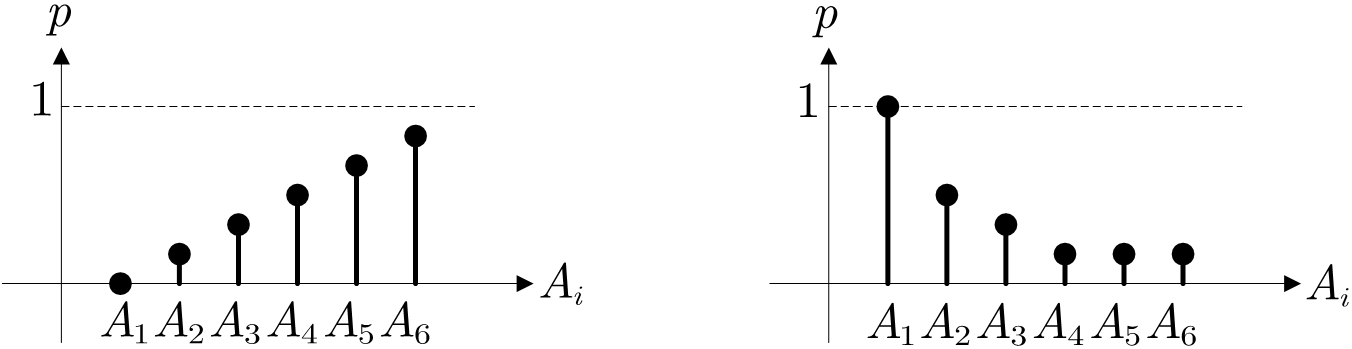
\includegraphics[height=2.5cm]{2.1.png}
\end{figure}

若记事件：
\begin{align*}
&A_1=\left\{ \text{点数能被}1\text{整除} \right\} \\
&A_2=\left\{ \text{点数能被}2\text{整除} \right\} \\
&A_3=\left\{ \text{点数能被}3\text{整除} \right\} \\
&A_4=\left\{ \text{点数能被}4\text{整除} \right\} \\
&A_5=\left\{ \text{点数能被}5\text{整除} \right\} \\
&A_6=\left\{ \text{点数能被}6\text{整除} \right\}
\end{align*}
则它们的概率用图形显示如上右图。
事件概率呈现依次递减的规律。

通过图形，我们可以直观地感受事件概率的分布规律，这就是本章要讨论的内容。






\newpage
\section{一维随机变量与分布函数}

本节介绍两个基本概念——一维随机变量和分布函数，为之后讨论奠定基础。

本节要点：
\begin{itemize}
    \item 深刻掌握一维随机变量的概念；
    \item 掌握分布函数的概念。
\end{itemize}

%============================================================
\subsection{一维随机变量的概念}

\begin{definition}[一维随机变量]
设随机试验$E$的样本空间为$\varOmega $，若每个样本点$\omega$均有唯一确定的实数$X$与之对应，则称$X$为{\bf 定义在$\varOmega $上的一维随机变量}，也称{\bf 随机变量}或简称{\bf 变量}。
\end{definition}

随机变量将对样本点的文字描述投射到实数，注意，这里投射的是样本点，或者说是基本事件，而非任意事件。
$X$的值在有些情况下可直观地赋予，如次品数量、人流数量、等待时间，但在有些情况下是人为赋予的，并没有特别的物理意义，如抛硬币的正反面，此时只要保证“唯一”、“确定”两个要求即可。

于是，我们将事件$A$及其概率$P\left( A \right) $和变量$X$的取值范围$D$的概率$P\left\{ X\in D \right\} $等价起来：
\[
\begin{array}{l}
	\omega\\
	A\\
	P\left( A \right)\\
\end{array}\Leftrightarrow \begin{array}{l}
	X\\
	X\in D\\
	P\left\{ X\in D \right\}\\
\end{array}
\]
一维随机变量可视作一种特殊的变量，虽然其取值范围可以为$\mathbb{R} $，但与普通变量相比有如下特殊性：
\begin{itemize}
    \item 根据具体试验，随机变量有意义的取值是人为设定且事先已知的；
    \item 但是在试验前，具体的取值无法预知；
    \item 我们能知道的是每个取值的概率。
\end{itemize}

%============================================================
\subsection{分布函数的概念}

\begin{definition}[分布函数]
设有随机变量$X$，对于$\forall x\in \mathbb{R} $，若$P\left\{ X\leqslant x \right\} $均有唯一的值与之对应，则称该对应关系为{\bf $X$的分布函数}，记作$F\left( x \right) $，即：
\[
F\left( x \right) := P\left\{ X\leqslant x \right\} ,\qquad x\in \mathbb{R}
\]
\end{definition}

分布函数描述了$X$每个取值之前（包括该值）的所有概率之和，所以分布函数的差可以描述变量在一个范围内的概率，即$X$在$\left( a,b \right] $的概率可以表示为：
\[
P\left\{ a<X\leqslant b \right\} =F\left( b \right) -F\left( a \right)
\]
分布函数的定义还隐含了判断一个函数能否被视为分布函数的充要条件：
\[
F\left( X \right) \text{是分布函数}\Leftrightarrow \begin{cases}
	0\leqslant F\left( x \right) \leqslant 1\\
	\underset{x\rightarrow -\infty}{\lim}F\left( x \right) =P\left( \oslash \right) =0\\
	\underset{x\rightarrow +\infty}{\lim}F\left( x \right) =P\left( \varOmega \right) =1\\
\end{cases}
\]
分布函数还有以下性质：
\begin{itemize}
    \item $F\left( x \right) $必单调增，即$x_1<x_2\Rightarrow F\left( x_1 \right) \leqslant F\left( x_2 \right) $；
    \item $F\left( x \right) $每个点$x_0$均右连续，即$\underset{x\rightarrow {x_0}^+}{\lim}F\left( x \right) =F\left( x_0 \right) $。
\end{itemize}

\begin{tcolorbox}
我们对分布函数的要求非常低，只需要满足3个条件即可，没有连续、可导的要求。
有些教材将充要条件视为分布函数的性质或定理，但其实这3个条件是概率的公理化定义的必然要求。
所以本笔记更倾向于将这3个条件视作公理化条件。
\end{tcolorbox}

这里需要理解$X,x$两者的区别。
$x$是普通变量，取值范围为$\mathbb{R} $，本身不承担物理意义，而$X$是随机变量，有意义的取值范围通过事件规定。
如投硬币中，我们规定$X=1$表示正面向上，$X=0$表示反面向上，$X$取0、1之外的值是没有意义的，或者说$P\left\{ X\ne 0\mathrm{or}1 \right\} =0$。

至此，我们将之前的概念和函数的概念统一了起来，我们用变量代替样本，用函数描述概率。
\begin{table}[h]
\centering
\caption{事件和变量}
\begin{tabular}{ll}
    \toprule
    \multicolumn{1}{c}{事件} & \multicolumn{1}{c}{变量}  \\
    \midrule
    样本点$\omega $ & 随机变量$X$\\
    样本空间$\varOmega $ & $\mathbb{R} $\\
    随机事件$A$ & 取值范围，如$\left\{ X=1 \right\} ,\left\{ X\geqslant b \right\} ,\left\{ a<X\leqslant b \right\} $\\
    概率$P\left( A \right) $ & 分布函数的差，如$P\left\{ a<X\leqslant b \right\} =F\left( b \right) -F\left( a \right) $\\
    \bottomrule
\end{tabular}
\end{table}

常用公式：
\begin{align*}
&P\left\{ X=a \right\} =F\left( a \right) -F\left( a^- \right) \\
&P\left\{ X>a \right\} =1-F\left( a \right) \\
&P\left\{ X\geqslant a \right\} =1-F\left( a^- \right) \\
&P\left\{ X<a \right\} =F\left( a^- \right) \\
&P\left\{ a<X<b \right\} =F\left( b^- \right) -F\left( a \right) \\
&P\left\{ a\leqslant X<b \right\} =F\left( b^- \right) -F\left( a^- \right) \\
&P\left\{ a\leqslant X\leqslant b \right\} =F\left( b \right) -F\left( a^- \right)
\end{align*}

%============================================================
\subsection{例}

\begin{example}
在抛硬币的试验中，记事件$A$表示正面向上，若令$X=\begin{cases}
	0,A\\
	1,\bar{A}\\
\end{cases}$，讨论$X$的分布函数$F\left( x \right) $。
\end{example}

解：

由古典概型的计算方法易得$P\left( A \right) =P\left( \bar{A} \right) =\frac{1}{2}$，于是$P\left\{ X=0 \right\} =P\left\{ X=1 \right\} =\frac{1}{2}$，可得分布函数的表达式和图形：

\begin{figure}[h]
\centering
    \begin{minipage}{0.48\linewidth}
    \[
    F\left( x \right) =\begin{cases}
        0,&		x<0\\
        \frac{1}{2},&		0\leqslant x<1\\
        1,&		x\geqslant 1\\
    \end{cases}
    \]
    \end{minipage}
\hfill
    \begin{minipage}{0.48\linewidth}
    \centerline{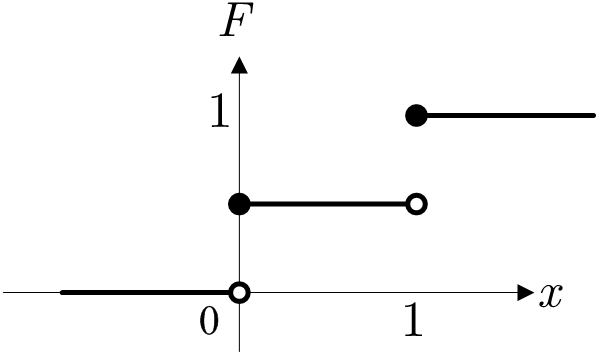
\includegraphics[width=4cm]{2.2.png}}
    \end{minipage}
\end{figure}
易见，$F\left( x \right) $在$x=0,1$有两个二类间断点，在间断点右连续。

~

\begin{example}
如有分布函数$F\left( x \right) =a+b\mathrm{arc}\tan x$，计算$P\left\{ -1<X\leqslant 0 \right\} $。
\end{example}

解：

题干的$F\left( x \right) $并不完整，需要计算$a,b$，根据分布函数的充要条件有：
\begin{align*}
&\because \begin{cases}
	\underset{x\rightarrow -\infty}{\lim}F\left( x \right) =a+b\cdot \frac{\pi}{2}=1\\
	\underset{x\rightarrow +\infty}{\lim}F\left( x \right) =a+b\cdot \left( -\frac{\pi}{2} \right) =0\\
\end{cases}\Rightarrow \begin{cases}
	a=\frac{1}{2}\\
	b=\frac{1}{\pi}\\
\end{cases} \\
&\therefore F\left( x \right) =\frac{1}{2}+\frac{1}{\pi}\mathrm{arc}\tan x \\
&\therefore P\left\{ -1<X\leqslant 0 \right\} =F\left( 0 \right) -F\left( -1 \right) =\frac{1}{2}-\left[ \frac{1}{2}+\frac{1}{\pi}\cdot \left( -\frac{\pi}{4} \right) \right] =\frac{1}{4}
\end{align*}






\newpage
\section{一维随机变量及其分布规律}

本节承上，深入讨论一维随机变量及其分布规律。
一维随机变量分为离散变量和连续变量，总体来讲它们是一样的，但在具体表达上又有不同的地方，其次，概率又是它们的函数。

本节要点：
\begin{itemize}
    \item 掌握一维离散型随机变量及其分布律的概念；
    \item 掌握一维连续型随机变量及其密度函数的概念；
    \item 了解一维随机变量函数的概念；
    \item 掌握离散变量函数的分布律的计算方法；
    \item 了解连续变量函数的密度函数的计算方法。
\end{itemize}


%============================================================
% 一维离散型随机变量及其分布律的概念
%============================================================
\subsection{一维离散型随机变量及其分布律的概念}

\begin{definition}[一维离散型随机变量]
若一维随机变量$X$的取值为有限个或可列无穷多个，则称$X$为{\bf 一维离散型随机变量}，简称{\bf 离散变量}。
设可能的取值为$x_1,x_2,\cdots ,x_i,\cdots $，且对应的概率记作：
\[
P\left\{ X=x_i \right\} =p_i
\]
称序列$p_i$为$X$的{\bf 分布律}或{\bf 概率分布}，可用表格展现，或记作：
\[
X\sim \left( \begin{matrix}
	x_1&		x_2&		\cdots&		x_i&		\cdots\\
	p_1&		p_2&		\cdots&		p_i&		\cdots\\
\end{matrix} \right)
\]
其中：
\begin{itemize}
    \item $x_i$：纯数学记号，对应基本事件$A_i$，通常为简化讨论，$x_i$取值为非负整数，分布律的计算通常基于上一章的讨论；
    \item $p_i=P\left\{ X=x_i \right\} =P\left( A_i \right) $：表示基本事件$A_i$的发生概率。
\end{itemize}
\end{definition}

若离散变量$X$有分布律$p_i$，则其分布函数为：
\[
F\left( x \right) =P\left\{ X\leqslant x \right\} =\sum_{x_i\leqslant x}{p_i}
\]
由分布函数的充要条件可得$p_i$成为分布律的充要条件：
\[
p_i\text{为分布律}\Leftrightarrow \begin{cases}
	p_i\geqslant 0\\
	\sum_i{p_i}=1\\
\end{cases}
\]


%============================================================
\subsection{一维连续型随机变量及其密度函数的概念}

\begin{definition}[一维连续型随机变量]
设一维随机变量$X$及其分布函数$F\left( x \right) $，若存在可积函数$f\left( x \right) \geqslant 0$，对于$\forall x$，有：
\[
F\left( x \right) =\int_{-\infty}^x{f\left( t \right) \cdot dt}
\]
则称$X$为{\bf 一维连续型随机变量}，简称{\bf 连续变量}，并称$f\left( x \right) $为$X$的{\bf 密度函数}或{\bf 概率密度}。
\end{definition}

\begin{tcolorbox}
注意，密度函数的定义不能采用$f\left( x \right) =F'\left( x \right) $，因为$F\left( x \right) $可以存在有限个不可导点，这并不违反分布函数的充要条件。
\end{tcolorbox}

由分布函数的充要条件易得$f\left( x \right) $成为密度函数的充要条件：
\[
f\left( x \right) \text{为密度函数}\Leftrightarrow \begin{cases}
	f\left( x \right) \geqslant 0\\
	\int_{-\infty}^{+\infty}{f\left( x \right) \cdot dx}=1\\
\end{cases}
\]
我们可以通过密度函数计算任意区间$\left( a,b \right] $的概率：
\[
P\left\{ a<X\leqslant b \right\} =\int_a^b{f\left( x \right) \cdot dx}
\]
其几何意义是其密度函数在$\left[ a,b \right] $区间和\textit{x}轴围成的曲边梯形的面积。

\begin{theorem}
若有连续变量$X$，则根据定义可知分布函数$F\left( x \right) $必连续，于是对于$F\left( x \right) $的可导点$x_0$，有：
\[
f\left( x_0 \right) =F'\left( x_0 \right)
\]
对于不可导点$x_0$，则可取$f\left( x_0 \right) $为任意非负实数。
反之也成立，即若$F\left( x \right) $不连续，则$X$不是连续型随机变量。
\end{theorem}

该定理隐含了两个含义。
首先对于存在不可导点的$F\left( x \right) $，$f\left( x \right) $表达并不唯一，其实将第一个定理结合微积分知识可知，若$f\left( x \right) $有有限个一类间断点，并不影响其积分。
其次，一维变量不是简单地分类为离散型和连续型，有些变量不是离散，但也找不到符合定义要求的密度函数。

\begin{theorem}
设连续变量$X$，则对于$\forall x_0\in \mathbb{R} $，有$P\left\{ X=x_0 \right\} =0$，即连续变量没有“单点概率”。
\end{theorem}

\begin{proof}
\begin{align*}
&\because P\left\{ X=x_0 \right\} =\int_{x_{0^-}}^{x_0}{f\left( x \right) \cdot dx} \\
&\because x_0=x_{0^-} \\
&\therefore P\left\{ X=x_0 \right\} =0
\end{align*}
其中第一个条件由分布函数定义$F\left( x \right) =P\left\{ X\leqslant x \right\} $保证，第二个条件由$X$的连续性保证。
\end{proof}

该定理更多的是描述一个常识，表达了$P\left\{ X=x_0 \right\} $和$f\left( x_0 \right) $是两个不同的概念。
几何上，$P\left\{ X=x_0 \right\} $是$f\left( x \right) $和点$x_0$围城的面积，自然是0，但这并不表示该点的概率密度为0。

\begin{theorem}
若连续变量$X$的密度函数$f\left( x \right) $为偶函数，则有：
\begin{itemize}
    \item $F\left( x \right) +F\left( -x \right) =1$
    \item $F\left( 0 \right) =\frac{1}{2}$
    \item $P\left\{ \left| X \right|\leqslant x \right\} =2F\left( x \right) -1$
\end{itemize}
\end{theorem}

\begin{proof}

~

式一：
\begin{align*}
&\because \begin{cases}
	F\left( x \right) =\int_{-\infty}^x{f\left( t \right) dt}\\
	F\left( -x \right) =\int_{-\infty}^{-x}{f\left( t \right) dt}\overset{u=-t}{=}\int_{+\infty}^x{f\left( -u \right) d\left( -u \right)}=\int_x^{+\infty}{f\left( u \right) du}\\
\end{cases} \\
&\therefore F\left( x \right) +F\left( -x \right) =\int_{-\infty}^x{f\left( t \right) dt}+\int_x^{+\infty}{f\left( t \right) dt}=\int_{-\infty}^{+\infty}{f\left( t \right) dt}=1
\end{align*}

式二，令$x=0$，略。

式三：
\begin{align*}
P\left\{ \left| X \right|\leqslant x \right\} &=\int_{-x}^x{f\left( t \right) dt}=2\int_0^x{f\left( t \right) dt}\\
&=2\left[ F\left( x \right) -F\left( 0 \right) \right] =2F\left( x \right) -1	
\end{align*}
\end{proof}


%============================================================
\subsection{分布律和密度函数的对比}

从函数的角度，分布律和密度函数都是函数，将随机变量空间映射到概率空间，或者说将事件映射到概率。

从变量定义的角度看，离散变量的定义从自身出发，而连续变量需要存在一个对应的可积函数，所以存在随机变量既不是离散的也不是连续的。

\begin{figure}[ht]
\centering
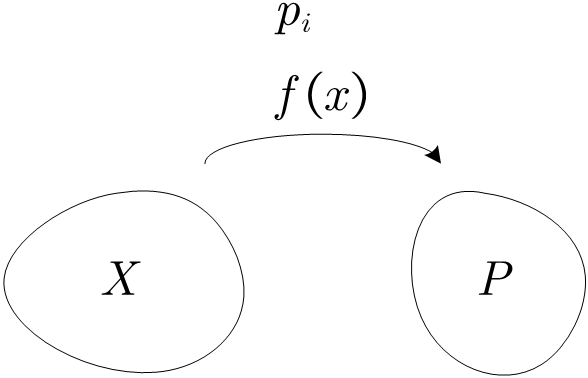
\includegraphics[height=2.5cm]{2.3.png}
\end{figure}

从概率角度看，事件的概率都是加权和，只是表达式不同，含义是相同的。
但离散变量有单点概率$P\left\{ X=x_i \right\} =p_i$，连续变量不存在单点概率$P\left\{ X=x_i \right\} =0$。
有些教材中，将分布律称为{\bf 概率质量函数}，将密度函数称为{\bf 概率密度函数}。
\begin{align*}
&P\left\{ a<X\leqslant b \right\} =\sum_{a<x\leqslant b}{p_i} \\
&P\left\{ a<X\leqslant b \right\} =\int_a^b{f\left( x \right) \cdot dx}
\end{align*}

从分布规律的角度看，无论是分布律还是密度函数，它们的充要条件都是概率公理化定义的必然要求。
\begin{align*}
&p_i\geqslant 0 &&\sum_i{p_i}=1 \\
&f\left( x \right) \geqslant 0 &&\int_{-\infty}^{+\infty}{f\left( x \right) \cdot dx}=1
\end{align*}

从应用角度出发，离散变量对应古典概型，如典型的抽样问题，连续变量对应几何概型，如碰面问题、人口分布问题。

%============================================================
\subsection{一维随机变量的函数的概念}

\begin{definition}[随机变量的函数]
设随机变量$X$及其取值范围$D$，$g\left( x \right) $定义在$D$上，若$Y=g\left( X \right) $依然为随机变量，则称$Y=g\left( X \right) $为{\bf 随机变量$X$的函数}。
\end{definition}

随机变量的函数这一概念可以对应复合函数。
一般来讲，随机变量的函数也可以是随机变量，但具体为离散变量还是连续变量就得视情况而定。

当$X$为离散变量时情况较为简单，$Y=g\left( X \right) $也为离散变量，$Y$的取值为$y_i=g\left( x_i \right) $，$Y$的分布律$P\left\{ Y=y_i \right\} $可由列表的方式计算，若$g\left( x_1 \right) =g\left( x_2 \right) $，则需要将相应概率相加$p_1+p_2$。

当$X$为连续变量时情况较为复杂，$Y$的密度函数由下列两个定理给出。

\begin{theorem}
设连续变量$X$有密度函数$f_X\left( x \right) ,X\in \mathbb{R} $，若$y=g\left( x \right) $在$\mathbb{R} $上严格单调，且反函数$x=g^{-1}\left( y \right) $具有连续的一阶导数，则$Y=g\left( X \right) $也是连续变量，且有密度函数：
\begin{align*}
&f_Y\left( y \right) =\begin{cases}
	f_X\left[ g^{-1}\left( y \right) \right] \cdot \left| \frac{dg^{-1}\left( y \right)}{dy} \right|,&		y\in \left( \alpha ,\beta \right)\\
	0,&		y\notin \left( \alpha ,\beta \right)\\
\end{cases} \\
&\alpha =\min \left\{ g\left( -\infty \right) ,g\left( +\infty \right) \right\} \\
&\beta =\max \left\{ g\left( -\infty \right) ,g\left( +\infty \right) \right\}
\end{align*}
\end{theorem}

\begin{theorem}
设连续变量$X$有密度函数$f_X\left( x \right) ,x\in \left[ a,b \right] $，当$x\notin \left[ a,b \right] $时$f_X\left( x \right) =0$，若$y=g\left( x \right) $在$\left[ a,b \right] $上严格单调，且反函数$x=g^{-1}\left( y \right) $具有连续的一阶导数，则$Y=g\left( X \right) $也是连续变量，且有密度函数：
\begin{align*}
&f_Y\left( y \right) =\begin{cases}
	f_X\left[ g^{-1}\left( y \right) \right] \cdot \left| \frac{dg^{-1}\left( y \right)}{dy} \right|,&		y\in \left[ \alpha ,\beta \right]\\
	0,&		y\notin \left[ \alpha ,\beta \right]\\
\end{cases} \\
&\alpha =\min \left\{ g\left( a \right) ,g\left( b \right) \right\} \\
&\beta =\max \left\{ g\left( a \right) ,g\left( b \right) \right\}
\end{align*}
\end{theorem}

严格单调保证了连续$X$能映射出一个连续的、单值的$Y$。
如分段函数，随单调但不严格，映射出的是离散的$Y$，又如绝对值函数，映射出连续的非单值$Y$。
若$y=g\left( x \right) $在定义域非单调，则$Y=g\left( X \right) $可能是离散型、连续型、不定型。

上述定理中，$\left| \frac{dg^{-1}\left( y \right)}{dy} \right|$是为了弥补空间变形带来的差异。
假设$X\sim U\left[ 0,1 \right] ,Y=\frac{1}{2}X$，则$f\left( x \right) =1,x\in \left[ 0,1 \right] $。
若我们简单地认为$f_Y\left( y \right) =f_X\left[ g^{-1}\left( y \right) \right] $，则有：
\begin{align*}
&f_Y\left( y \right) =f_X\left[ g^{-1}\left( y \right) \right] =1 \\
&\int_0^{1/2}{f_Y\left( y \right) dy}=\int_0^{1/2}{dy}=\frac{1}{2}
\end{align*}
显然违背了密度函数的充要条件，其原因在于$Y=\frac{1}{2}X$时，$dy\ne dx$，正确的做法是需要保证：
\[
f_Y\left( y \right) \left| dy \right|=f_X\left( x \right) \left| dx \right|
\]
此处，由于$y=g\left( x \right) $可能单调减，所以$dy,dx$都带上绝对值。
于是：
\[
f_Y\left( y \right) =f_X\left( x \right) \left| \frac{dx}{dy} \right|=f_X\left( x \right) \left| \frac{dg^{-1}\left( y \right)}{dy} \right|
\]


%============================================================
\subsection{例}

\begin{example}
设有8个正品，2个次品，若不放回地依次取出若干个，分析首次取到正品时所取产品个数的分布规律。
\end{example}

解：

该问题是抽样问题，由题干可知，首次取到正品只可能是抽了1、2、3个，抽取到$n\geqslant 4$个样品时，第$n$次不可能是首次抽到正品。
于是：
\begin{align*}
&P\left\{ X=1 \right\} =\frac{8}{10}=\frac{4}{5} \\
&P\left\{ X=2 \right\} =\frac{2}{10}\cdot \frac{8}{9}=\frac{8}{45} \\
&P\left\{ X=3 \right\} =\frac{2}{10}\cdot \frac{1}{9}\cdot \frac{8}{8}=\frac{1}{45}
\end{align*}
分布律：
\[
X\sim \left( \begin{matrix}
	1&		2&		3\\
	\frac{4}{5}&		\frac{8}{45}&		\frac{1}{45}\\
\end{matrix} \right)
\]
分布函数：
\[
F\left( x \right) =\begin{cases}
	0,&		x<1\\
	\frac{4}{5},&		1\leqslant x<2\\
	\frac{4}{5}+\frac{8}{45}=\frac{44}{45},&		2\leqslant x<3\\
	\frac{4}{5}+\frac{8}{45}+\frac{1}{45}=1,&		x\geqslant 3\\
\end{cases}
\]

~

\begin{example}
若离散变量$X$有分布律：
\[
X\sim \left( \begin{matrix}
	-1&		0&		1&		2\\
	\frac{1}{4}&		\frac{1}{6}&		\frac{1}{4}&		\frac{1}{3}\\
\end{matrix} \right)
\]
分析$Y=X^2$的分布律。
\end{example}

解：

\[
Y=\begin{cases}
	0,&		X=0\\
	1,&		X=\pm 1\\
	4,&		X=2\\
\end{cases}
\]

由于$P\left\{ Y=1 \right\} =P\left\{ X=-1 \right\} +P\left\{ X=1 \right\} =\frac{1}{4}+\frac{1}{4}$，得：
\[
Y\sim \left( \begin{matrix}
	0&		1&		4\\
	\frac{1}{6}&		\frac{1}{4}+\frac{1}{4}&		\frac{1}{3}\\
\end{matrix} \right)
\]

~

\begin{example}
若离散变量$X$有分布律$p_i=\frac{1}{2^i},i=1,2,\cdots $，试分析$Y=\sin \left( \frac{\pi}{2}X \right) $的分布律。
\end{example}

解：

由题干可得，$X$的取值为$1,2,\cdots $，可得$Y$的取值：
\begin{itemize}
    \item 当$X$取$1,5,\cdots $时，$Y=1$；
    \item 当$X$取$2,4,6,\cdots $时，$Y=0$；
    \item 当$X$取$3,7,\cdots $时，$Y=-1$。
\end{itemize}
\begin{align*}
P\left\{ Y=1 \right\} &=P\left\{ X=1 \right\} +P\left\{ X=5 \right\} +P\left\{ X=9 \right\} +\cdots \\
&=\frac{1}{2^1}+\frac{1}{2^5}+\frac{1}{2^9}+\cdots =\frac{\frac{1}{2}}{1-\frac{1}{2^4}}=\frac{8}{15} \\
P\left\{ Y=0 \right\} &=P\left\{ X=2 \right\} +P\left\{ X=4 \right\} +P\left\{ X=6 \right\} +\cdots \\
&=\frac{1}{2^2}+\frac{1}{2^4}+\frac{1}{2^6}+\cdots =\frac{\frac{1}{4}}{1-\frac{1}{2^2}}=\frac{1}{3} \\
P\left\{ Y=-1 \right\} &=P\left\{ X=3 \right\} +P\left\{ X=7 \right\} +P\left\{ X=11 \right\} +\cdots \\
&=\frac{1}{2^3}+\frac{1}{2^7}+\frac{1}{2^{11}}+\cdots =\frac{\frac{1}{2^3}}{1-\frac{1}{2^4}}=\frac{2}{15}
\end{align*}






\newpage
\section{常见的分布律和密度函数}

本节介绍几个常见的分布规律，大多数实际问题都可以归结到本节介绍的这些分布规律。

本节要点：
\begin{itemize}
    \item 理解5个常见的分布律及其应用场景；
    \item 理解3个常见的密度函数及其应用场景；
    \item 学会用这8个分布规律考察实际问题。
\end{itemize}

%============================================================
\subsection{0-1分布}

{\bf 0-1分布}又称{\bf 两点分布}，记作$B\left( 1,p \right) $，描述最简单的分布：
\begin{align*}
&P\left\{ X=1 \right\} =p\\
&P\left\{ X=0 \right\} =1-p
\end{align*}
更普遍地记作：
\[
P\left\{ X=x \right\} =p^x\left( 1-p \right) ^{1-x},\qquad \begin{array}{l}
	x=0,1\\
	p\in \left( 0,1 \right)\\
\end{array}
\]
其中：
\begin{itemize}
    \item $x$：一般取0表示事件不发生，1表示事件发生；
    \item $p$：表示事件发生的概率。
\end{itemize}
特别地，当$p=0\mathrm{or}1$时称为{\bf 常数分布}。
常数分布表示了事件100\%发生，所以无实际用途，只是为了完善概念而提出。

\begin{tcolorbox}
一般如果试验中只有两个样本点，非黑即白、非正即负，我们就可以用两点分布描述。
两点分布的使用场景非常少。
\end{tcolorbox}

%============================================================
\subsection{二项分布}

{\bf 二项分布}又称{\bf 伯努利分布}，记作$B\left( n,p \right) $，因其分布律表达式中包含二项式系数而得名，描述$n$重伯努利试验中具有发生概率$p$的事件发生$x$次的概率的分布规律：
\[
P\left\{ X=x \right\} =C_{n}^{x}p^x\left( 1-p \right) ^{n-x},\qquad \begin{array}{l}
	x=0,1,\cdots ,n\\
	p\in \left( 0,1 \right)\\
\end{array}
\]
其中：
\begin{itemize}
    \item $x$：表示事件发生的次数，包括一次也不发生（$x=0$）和每次都发生（$x=n$）；
    \item $p$：表示事件发生的概率；
    \item $C_{n}^{x}$：$n$次子试验中，事件发生了$x$次的次数，注意，这里用组合，表示我们只关心$x$次，而不关心具体是哪$x$次；
    \item $p^x$：表示事件发生$x$次的概率；
    \item $\left( 1-p \right) ^{n-x}$：表示其余$n-x$次子试验中事件不发生的概率。
\end{itemize}
伯努利试验中，小概率事件倾向于少发生，大概率事件倾向于多次发生，且发生概率最大的在$np$次。

\begin{figure}[h]
\centering
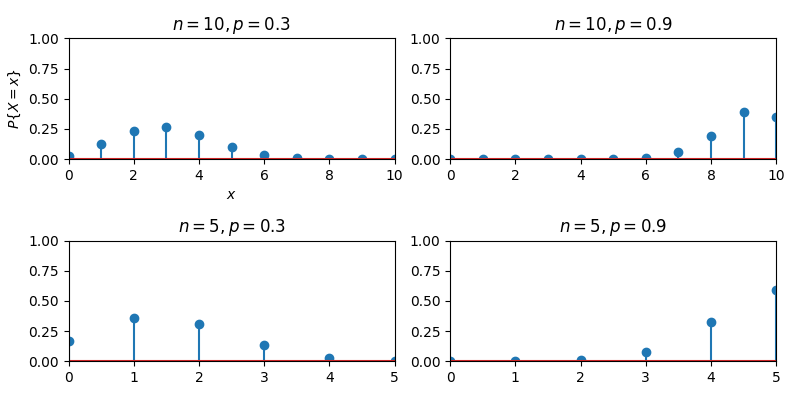
\includegraphics[height=5cm]{2.4.png}
\caption{二项分布}
\end{figure}

\begin{tcolorbox}
二项分布描述伯努利试验，我们可以知道在固定$n$次子试验中，事件$A$发生几次的概率是最大的。
最典型的应用就是$n$次放回抽样，计算抽到$x$个次品的概率。
\end{tcolorbox}

%============================================================
\subsection{泊松分布}

{\bf 泊松分布}，记作$P\left( \lambda \right) $，因由法国数学家Siméon-Denis Poisson发表而得名，一般用于近似描述一定时间内，某个稀有事件发生次数的概率分布：
\[
P\left\{ X=x \right\} =\frac{\lambda ^x}{x!}e^{-\lambda},\qquad \begin{array}{l}
	x=0,1,2,\cdots\\
	\lambda >0\\
\end{array}
\]
其中：
\begin{itemize}
    \item $\lambda =np$：$n$表示总次数，$p$表示事件发生的概率，一般$n$很大，$p$很小，两者乘积$\lambda $适中；
    \item $x$：表示事件发生的次数。
\end{itemize}
泊松分布中，发生概率最大的在$\lambda $次。

\begin{figure}[h]
\centering
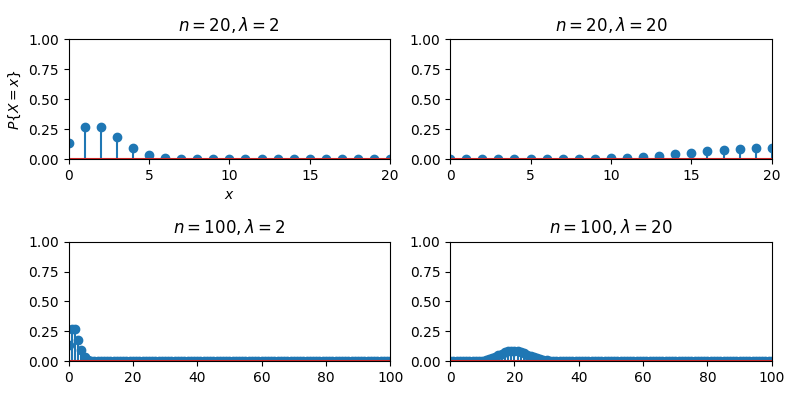
\includegraphics[height=5cm]{2.5.png}
\caption{泊松分布}
\end{figure}

\begin{theorem}[泊松定理]
在$n$重伯努利试验中，事件$A$在每次试验中发生概率为$p_n\in \left( 0,1 \right) $，且$p_n$和试验次数$n$有关，若$\underset{n\rightarrow \infty}{\lim}np_n=\lambda >0$，则对于$\forall k\geqslant 0$，必有：
\[
\underset{n\rightarrow \infty}{\lim}C_{n}^{x}{p_n}^x\left( 1-p_n \right) ^{n-x}=\frac{\lambda ^x}{x!}e^{-\lambda}
\]
\end{theorem}

该定理揭示了二项分布和泊松分布的关系，当$n$充分大，$p$很小，且$\lambda $适中时，二项分布近似于泊松分布。
证明见“教材\cite{book1}”的P44，例2.2.7，着重理解条件$\underset{n\rightarrow \infty}{\lim}np_n=\lambda $在证明过程中的使用。

\begin{tcolorbox}
泊松分布依然基于伯努利试验，和二项分布的区别在于长时间段和稀有事件，是二项分布的近似，常用于描述如某个时间段内商场人数、候车站人数、机器故障、灾害发生等。
\end{tcolorbox}

%============================================================
\subsection{几何分布}

{\bf 几何分布}，记作$G\left( p \right) $，因其分布律表达式中含有几何级数因子而得名，描述事件$A$首次发生时所进行的试验次数服从的分布：
\[
P\left\{ X=x \right\} =p\left( 1-p \right) ^{x-1},\qquad \begin{array}{l}
	x=1,2,\cdots\\
	p\in \left( 0,1 \right)\\
\end{array}
\]
其中：
\begin{itemize}
    \item $x$：表示事件$A$在第$x$次子试验时发生；
    \item $p$：表示事件$A$发生的概率；
    \item $\left( 1-p \right) ^{x-1}$：表示前面$x-1$次子试验中事件$A$均不发生的概率。
\end{itemize}
几何分布中，$p$越大，事件越倾向于早发生。
几何分布有性质：
\[
P\left\{ X>m+n \middle| X>m \right\} =P\left\{ X>n \right\}
\]

\begin{figure}[h]
\centering
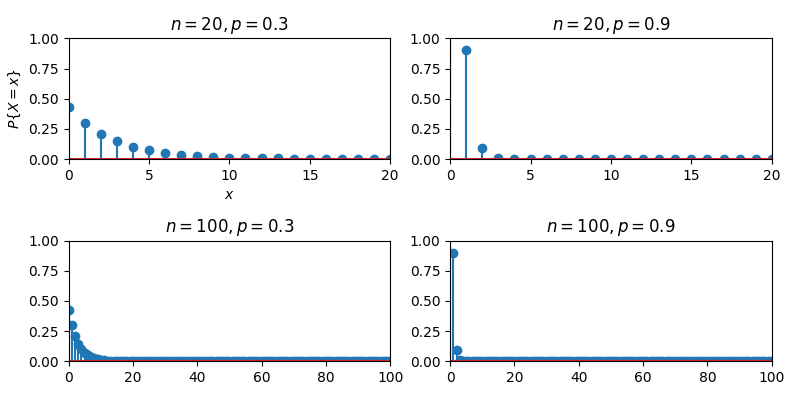
\includegraphics[height=5cm]{2.6.png}
\caption{几何分布}
\end{figure}

\begin{tcolorbox}
几何分布依然基于伯努利试验。
几何分布不规定具体几次试验，而是着重刻画“首次即停止”，即事件$A$在前几次子试验中均不发生，在第$n$次子试验时首次发生的概率。
几何分布在现实中使用不多，在连续型随机变量中对应指数分布，常用来描述设备无故障运行时间的概率分布。
\end{tcolorbox}

考察二项分布和几何分布
\begin{align*}
&B\left( n,p \right) && P\left\{ X=x \right\} =C_{n}^{x}p^x\left( 1-p \right) ^{n-x}, x=0,1,\cdots ,n \\
&G\left( p \right)   && P\left\{ X=x \right\} =p\left( 1-p \right) ^{x-1}, x=1,2,\cdots
\end{align*}
不难发现，$\left( 1-p \right) ^{n-x},\left( 1-p \right) ^{x-1}$有类似互为倒数的关系，所以几何分布又被称为{\bf 负二项分布}。

%============================================================
\subsection{超几何分布}

{\bf 超几何分布}，记作$H\left( M,N,n \right) $，因其分布律与超几何函数的级数展开式的系数类似而得名，描述不放回抽取试验，从$N$个样品中抽取$n$个，出现$x$个次品的概率分布：
\[
P\left\{ X=x \right\} =\frac{C_{N-M}^{n-x}C_{M}^{x}}{C_{N}^{n}}, \begin{array}{l}
	N>1,M\leqslant N\\
	n\leqslant N,x\in \left[ \max \left\{ 0,M+n-N \right\} ,\min \left\{ M,n \right\} \right]\\
\end{array}
\]
其中：
\begin{itemize}
    \item $N,M$：共$N$个样品，其中有$M$个次品；
    \item $n,x$：抽取$n$个，其中$x$个为次品。
\end{itemize}
超几何分布中，抽到$\frac{M}{N}\cdot n$的概率最大。

\begin{figure}[h]
\centering
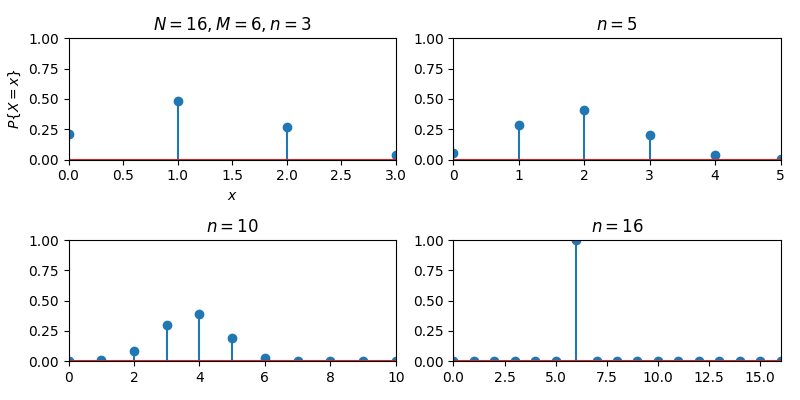
\includegraphics[height=5cm]{2.7.png}
\caption{超几何分布，16个样品，6个次品}
\end{figure}
\begin{figure}[h]
\centering
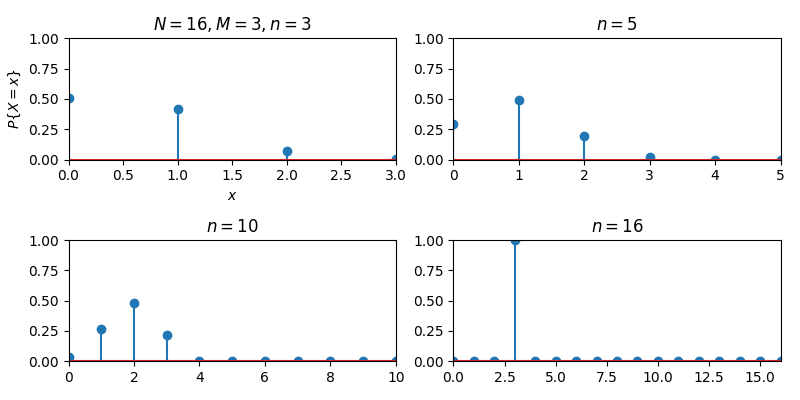
\includegraphics[height=5cm]{2.8.png}
\caption{超几何分布，16个样品，3个次品}
\end{figure}

\begin{tcolorbox}
超几何分布描述“不放回”抽取试验，不是基于伯努利试验，描述抽到$x$个次品的概率分布。
\end{tcolorbox}

%============================================================
\subsection{均匀分布}

{\bf 均匀分布}，记作$U\left[ a,b \right] $，描述了最简单的分布：
\[
f\left( x \right) =\begin{cases}
	\frac{1}{b-a},&		x\in \left[ a,b \right]\\
	0,&		x\notin \left[ a,b \right]\\
\end{cases}\qquad F\left( x \right) =\begin{cases}
	0,&		x\in \left( -\infty ,a \right)\\
	\frac{1}{b-a}\cdot \left( x-a \right) ,&		x\in \left[ a,b \right)\\
	1,&		x\in \left[ b,+\infty \right)\\
\end{cases}
\]

\begin{tcolorbox}
均匀分布对应几何概型，在自然界十分罕见，常用于人工事件，如设计的随机数发生器需尽量满足均匀分布。
\end{tcolorbox}

%============================================================
\subsection{指数分布和威布尔分布}

{\bf 指数分布}，记作$E\left( \lambda \right) $，和几何分布类似，描述事件$A$首次发生的时间：
\[
f\left( x \right) =\begin{cases}
	0,&		x<0\\
	\lambda e^{-\lambda x},&		x\geqslant 0\\
\end{cases}\qquad F\left( x \right) =\begin{cases}
	0,&		x<0\\
	1-e^{-\lambda x},&		x\geqslant 0\\
\end{cases}
\]
其中：
\begin{itemize}
    \item $\lambda $：常称作{\bf 趋近率}， 越小，趋近越慢。
\end{itemize}
指数分布的推导见“教材\cite{book2}”P52，详细阅读，可加深对$\lambda $的理解。

\begin{figure}[h]
\centering
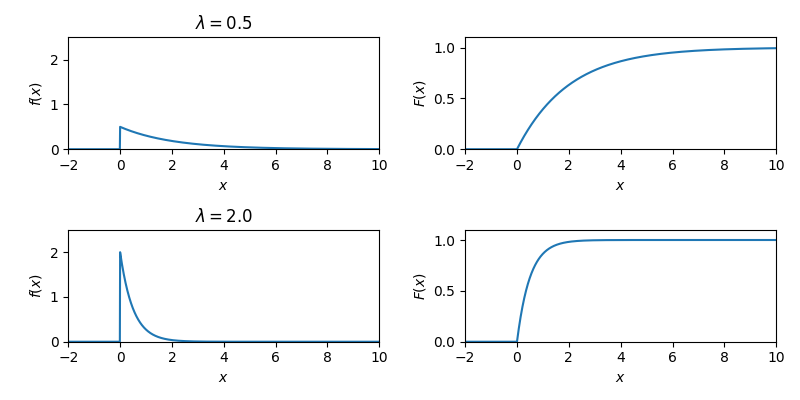
\includegraphics[height=5cm]{2.9.png}
\caption{均匀分布}
\end{figure}

\begin{tcolorbox}
指数分布对应离散变量的几何分布，是几何分布的连续模型，常用于描述元器件的寿命。
\end{tcolorbox}

描述元件故障时，我们用事件$A$表示元件发生故障，随机变量$X$表示元件的工作寿命，此时$\lambda $也被称为{\bf 失效率}，$\lambda $越大，表示元器件的寿命越短，通常我们会说某元件的使用寿命数服从$\lambda $指数分布。
元件能无故障运行$x$小时的概率，即$x$小时内事件$A$不发生的概率$P\left( \bar{A} \right) $，对应的分布函数为$1-F\left( x \right) $。

~

\begin{theorem}
若$X\sim E\left( \lambda \right) $，则有：
\[
P\left\{ X>s+t \middle| X>s \right\} =P\left\{ X>t \right\}
\]
\end{theorem}

\begin{proof}
\begin{align*}
&\because P\left\{ X>x_0 \right\} =1-F\left( x_0 \right) =1-\left( 1-e^{-\lambda x_0} \right) =e^{-\lambda x_0} \\
&\because P\left\{ X>s+t \middle| X>s \right\} =\frac{P\left\{ X>s+t\cap X>s \right\}}{P\left\{ X>s \right\}}=\frac{P\left\{ X>s+t \right\}}{P\left\{ X>s \right\}} \\
&\therefore P\left\{ X>s+t \middle| X>s \right\} =\frac{e^{-\lambda \left( s+t \right)}}{e^{-\lambda s}}=e^{-\lambda t}
\end{align*}
\end{proof}

从该性质可见，指数分布的概率和“起点”无关。
这个性质在描述元器件寿命时和实际情况不符。
实际情况中，随着使用时间的增加，元器件寿命会“加速缩短”。
反映到失效率$\lambda $，不会是一个常数，而是会随着使用而逐渐变大。
考虑到这一因素，人们引入了{\bf 威布尔分布}，因瑞典工程师、数学家Waloddi Weibull（1887-1979）详细解释了这一分布而得名，其密度函数和分布函数如下：
\[
f\left( x \right) =\begin{cases}
	0,&		x<0\\
	\lambda \alpha x^{\alpha -1}e^{-\lambda x^{\alpha}},&		x\geqslant 0\\
\end{cases}\qquad F\left( x \right) =\begin{cases}
	0,&		x<0\\
	1-e^{-\lambda x^{\alpha}},&		x\geqslant 0\\
\end{cases}
\]
指数分布是$\alpha =1$时的特列。

%============================================================
\subsection{正态分布}

{\bf 正态分布}，也称{\bf 高斯分布}，记作$N\left( \mu ,\sigma ^2 \right) $，类似泊松分布，描述一个范围内的分布情况：
\[
f\left( x \right) =\frac{1}{\sqrt{2\pi}\sigma}e^{-\frac{\left( x-\mu \right) ^2}{2\sigma ^2}},\qquad \mu \in \mathbb{R} ,\sigma >0
\]
其中：
\begin{itemize}
    \item $\mu $：数学期望，规定了中心点的横坐标，$f\left( x \right) $以$x=\mu $为对称，并在$x=\mu $取得最大值$\frac{1}{\sqrt{2\pi}\sigma}$；
    \item $\sigma $：标准差，一方面规定了$f\left( x \right) $的两个拐点$\mu \pm \sigma $，另一方面也规定了平坦度，$\sigma $越大，曲线越平坦。
\end{itemize}
特别地，当$\mu =0,\sigma =1$时，称为{\bf 标准正态分布}，记作$N\left( 0,1 \right) $，此时密度函数和分布函数通常记为$\varphi \left( x \right) ,\varPhi \left( x \right) $，有：
\[
\varphi \left( x \right) =\frac{1}{\sqrt{2\pi}}e^{-\frac{x^2}{2}}\qquad \varPhi \left( x \right) =\int_{-\infty}^x{\varphi \left( t \right) \cdot dt}
\]
根据密度函数的偶函数定理，有性质：
\begin{align*}
&\varPhi \left( x \right) +\varPhi \left( -x \right) =1 \\
&\varPhi \left( 0 \right) =0.5
\end{align*}

\begin{figure}[h]
\centering
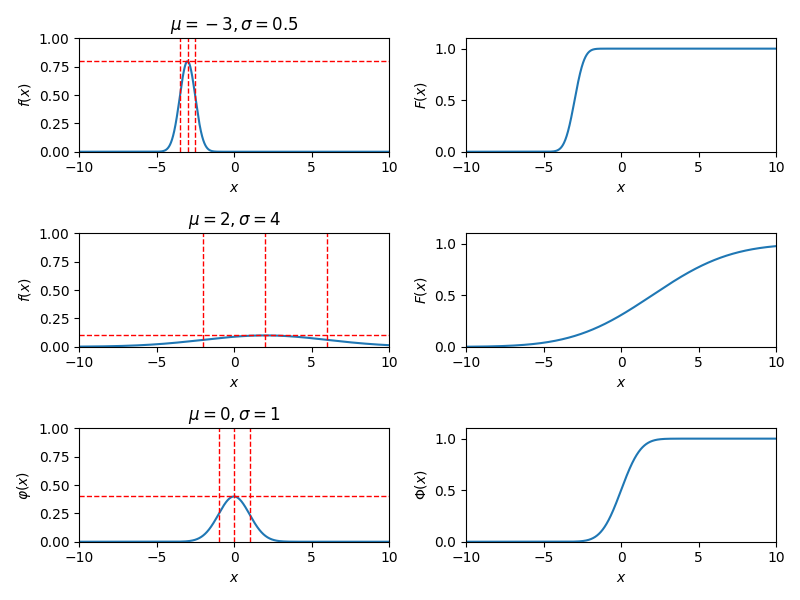
\includegraphics[height=7.5cm]{2.10.png}
\caption{正态分布}
\end{figure}

\begin{tcolorbox}
正态分布常用于描述身高、体重、成绩、元器件指标等的离散程度。
\end{tcolorbox}

\begin{theorem}
若$X\sim N\left( \mu ,\sigma ^2 \right) $，则有：
\[
P\left\{ a<X\leqslant b \right\} =\varPhi \left( \frac{b-\mu}{\sigma} \right) -\varPhi \left( \frac{a-\mu}{\sigma} \right)
\]
\end{theorem}

可用积分变量替换进行证明，略。
该定理使得我们可以用标准分布计算任何正态分布。

\begin{theorem}
设$X_1\sim N\left( \mu _1,{\sigma _1}^2 \right) ,X_2\sim N\left( \mu _2,{\sigma _2}^2 \right) $ ，则$Y=X_1+X_2$也服从正态分布，且有：
\begin{align*}
&Y\sim N\left( \mu _1+\mu _2,{\sigma _1}^2+{\sigma _2}^2 \right) \\
&f\left( y \right) =\frac{1}{\sqrt{2\pi \left( {\sigma _1}^2+{\sigma _2}^2 \right)}}e^{-\frac{\left[ y-\left( \mu _1+\mu _2 \right) \right] ^2}{2\left( {\sigma _1}^2+{\sigma _2}^2 \right)}}
\end{align*}
反之，若正态分布$Y$能表示成两个变量的和$Y=X_1+X_2$，则$X_1,X_2$也必然是正态分布，这点被称为正态分布的{\bf 再生性}。
\end{theorem}

\begin{tcolorbox}
正态分布有很多特别的表现。
一方面，若足够多的独立分布叠加，则总体可看成正态分布；另一方面，在相同方差的情况下，正态分布具有最大的不确定性。
所以正态分布不但非常常见，而且也是优先考虑使用的模型。
\end{tcolorbox}

%============================================================
\subsection{常见分布的总结}

\begin{table}[h]
\centering
\caption{常见分布总结}
\begin{tabular}{ll}
    \toprule
    \multicolumn{1}{c}{分布} & \multicolumn{1}{c}{含义、用途}  \\
    \midrule
    0-1分布$B\left( 1,p \right) $ & 最简单的分布，非黑即白。\\
    二项分布$B\left( n,p \right) $ & $n$重伯努利试验中发生$x$次的概率分布。\\
    泊松分布$P\left( \lambda \right) $ & 同上，重在非常多次和小概率。\\
    几何分布$G\left( p \right) $ & 同上，事件首次发生时次数的概率分布。\\
    超几何分布$H\left( M,N,n \right) $ & 不放回抽取中，抽到含$x$个次品的概率分布。\\
    均匀分布$U\left[ a,b \right] $ & 常用于人工事件，自然界极为罕见。\\
    指数分布$E\left( \lambda \right) $ & 常用于描述元器件寿命。\\
    正态分布$N\left( \mu ,\sigma ^2 \right) $ & 描述某指标的离散度。\\
    \bottomrule
\end{tabular}
\end{table}


%============================================================
% 例
%============================================================
\subsection{例}

\begin{example}
设某射手独立地向目标射击4次，每次击中的概率为0.6，问射击几次的击中概率最大。
\end{example}

解：

这是4重伯努利试验，且射击次数 服从二项分布，有：
\[
P\left\{ X=k \right\} =C_{n}^{k}p^k\left( 1-p \right) ^{n-k}=C_{4}^{k}0.6^k\left( 1-0.6 \right) ^{4-k}
\]
经计算可得，$X=2\mathrm{or}3$时，概率最大，可达0.3456。

~

\begin{example}
某产品的次品率为0.5\%，若取1000件，计算不多于5件次品的概率。
\end{example}

解：

可以认为是$n$重伯努利试验，使用二项分布，由于次数很多概率很小，所以可以用泊松分布作近似计算，取$\lambda =np=1000\cdot 0.005=5$：
\begin{align*}
&\because P\left\{ X=x \right\} =\frac{\lambda ^x}{x!}e^{-\lambda} \\
&\therefore P\left\{ X\leqslant 5 \right\} =\sum_{x=0}^5{\frac{5^x}{x!}e^{-5}}=0.615961
\end{align*}

~

\begin{example}
若有均匀分布的变量$X\sim U\left[ 1,6 \right] $，则方程$x^2+Xx+1=0$有实根的概率。
\end{example}

解：

方程有实根必须满足$\Delta =X^2-4\geqslant 0$，即$X\leqslant -2 \mathrm{or} X\geqslant 2$。
由于$X\thicksim U\left[ 1,6 \right] $，所以有实根的概率即求分布$P\left\{ 2\leqslant X\leqslant 6 \right\} $的值：
\[
P\left\{ 2\leqslant X\leqslant 6 \right\} =F\left( 6 \right) -F\left( 2^- \right) =\frac{6-1}{6-1}-\frac{2-1}{6-1}=\frac{4}{5}
\]
进一步，分析有两个不同实根，$\Delta =X^2-4>0\Rightarrow X<-2\mathrm{or}X>2$：
\[
P\left\{ 2<X\leqslant 6 \right\} =F\left( 6 \right) -F\left( 2 \right) =\frac{6-1}{6-1}-\frac{2-1}{6-1}=\frac{4}{5}
\]
有实根和有不同实根的概率相同，这点也可以由$P\left\{ X=2 \right\} =0$得到。

~

\begin{example}
某仪器由3个电子元件组成，元件工作寿命符合$\lambda =1/600$的指数分布，单位小时，且元件质量和运行相互独立。
\begin{enumerate}
    \item 若元件逻辑上“串联”，即仪器需要3个电子元件均正常才能工作；
    \item 若元件相互热备，即只需要一个元件能工作，仪器就能正常工作，
\end{enumerate}
试分析仪器的寿命分布。
\end{example}

解：

我们用事件$A_i$第$i$个元件出现问题的时间的概率，于是：
\[
P\left( A_i \right) =P\left\{ X\leqslant x \right\} =F\left( x \right) =1-e^{-\lambda x}
\]

1. 当元件逻辑上“串联”时，仪器的运行取决于3个元件都不能有故障，即$\bar{A}=\bar{A}_1\bar{A}_2\bar{A}_3$，于是：
\begin{align*}
P\left( \bar{A} \right) &=P\left( \bar{A}_1\bar{A}_2\bar{A}_3 \right) =P\left( \bar{A}_1 \right) P\left( \bar{A}_2 \right) P\left( \bar{A}_3 \right) \\
&=\left[ 1-P\left( A_1 \right) \right] \left[ 1-P\left( A_2 \right) \right] \left[ 1-P\left( A_3 \right) \right] \\
&=e^{-3\lambda x}=e^{-\frac{x}{200}}
\end{align*}

2. 当元件相互热备时，仪器的运行只需要任意一个元件能正常运行即可，即$\bar{A}=\bar{A}_1+\bar{A}_2+\bar{A}_3=\overline{A_1A_2A_3}=\varOmega -A_1A_2A_3$：
\begin{align*}
P\left( \bar{A} \right) &=1-P\left( A_1A_2A_3 \right) =1-P\left( A_1 \right) P\left( A_2 \right) P\left( A_3 \right) \\
&=1-\left( 1-e^{-\lambda x} \right) ^3=1-\left( 1-e^{-\frac{x}{600}} \right) ^3
\end{align*}

\begin{figure}[h]
\centering
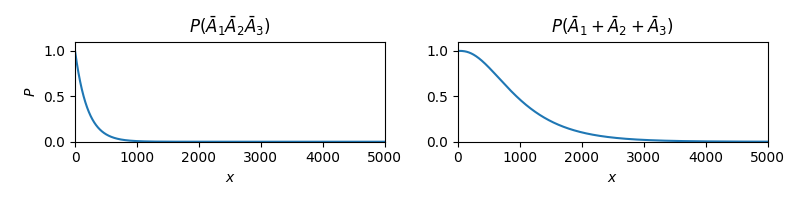
\includegraphics[height=2.3cm]{2.11.png}
\end{figure}

左图为串联，右图为热备，横坐标表示时间，单位小时，纵坐标表示无故障运行时间的概率。

~

\begin{example}
若随机变量服从正态分布$X\sim N\left( \mu ,\sigma ^2 \right) $，计算$P\left\{ \left| X-\mu \right|<k\sigma \right\} $。
\end{example}

解：

\begin{align*}
P\left\{ \left| X-\mu \right|<k\sigma \right\} &=P\left\{ -k\sigma +\mu <X<k\sigma +\mu \right\} \\
&=P\left\{ a<X\leqslant b \right\} \\
&=\varPhi \left( \frac{\left( k\sigma +\mu \right) -\mu}{\sigma} \right) -\varPhi \left( \frac{\left( -k\sigma +\mu \right) -\mu}{\sigma} \right) \\
&=\varPhi \left( \frac{k\sigma}{\sigma} \right) -\varPhi \left( \frac{-k\sigma}{\sigma} \right) =\varPhi \left( k \right) -\varPhi \left( -k \right) \\
&=2\varPhi \left( k \right) -1
\end{align*}
特别地：
\begin{align*}
&P\left\{ \left| X-\mu \right|<\sigma \right\} =0.6826 \\
&P\left\{ \left| X-\mu \right|<2\sigma \right\} =0.9544
\end{align*}
也即中心点$\mu $左右$\sigma $范围内占据了一半稍微多一点，而$2\sigma $范围内占据了绝大部分。

~

\begin{example}
设电压服从正态分布$V\sim N\left( 220,25^2 \right) $，若某电子元件在电压小于200V时失效的概率为0.1，在$\left[ 200,240 \right] $失效的概率为0.001，在大于240V时失效概率为0.2。
分析：
\begin{enumerate}
    \item 电子元件失效的概率，
    \item 当元件损坏时，电压不正常（不在$\left[ 200,240 \right] $范围内）的概率。
\end{enumerate}
\end{example}

解：

记$A_1,A_2,A_3$表示电压落在3个区间事件，则：
\begin{align*}
P\left( A_1 \right) &=P\left\{ X<200 \right\} =\varPhi \left( \frac{200-220}{25} \right) \\
&=\varPhi \left( -0.8 \right) =1-\varPhi \left( 0.8 \right) =0.2119 \\
P\left( A_2 \right) &=P\left\{ 200\leqslant X\leqslant 240 \right\} \\
&=\varPhi \left( \frac{240-220}{25} \right) -\varPhi \left( \frac{200-220}{25} \right) =0.5762 \\
P\left( A_3 \right) &=P\left\{ X>240 \right\} =1-\varPhi \left( \frac{240-220}{25} \right) =0.2119
\end{align*}
且构成电压分布的完备组。

1. 记$B$表示元件失效，则由全概率公式易得：
\begin{align*}
P\left( B \right) &=\sum_{i=1}^3{P\left( A_i \right) P\left( B \middle| A_i \right)} \\
&=0.2119\cdot 0.1+0.5762\cdot 0.001+0.2119\cdot 0.2 \\
&=0.0641
\end{align*}

2. 使用贝叶斯公式：
\begin{align*}
P\left( A_1 \middle| B \right) +P\left( A_3 \middle| B \right) &=\frac{P\left( A_1 \right) P\left( B \middle| A_1 \right)}{P\left( B \right)}+\frac{P\left( A_3 \right) P\left( B \middle| A_3 \right)}{P\left( B \right)} \\
&=\frac{0.2119\cdot 0.1}{0.0641}+\frac{0.2119\cdot 0.2}{0.0641} \\
&=0.991732
\end{align*}
可见，电压不正常占据了绝大多数可能性。

~

\begin{example}
用车床加工半径为$2\mathrm{mm}$的圆柱形零件，若加工刀具径向离散度在$\pm 0.1\mathrm{mm}$均匀分布，求零件截面面积的离散度分布。
\end{example}

解：

由题干可知，零件半径在加工时的分布为$R\sim U\left[ 1.9,2.1 \right] $，密度函数：$f_R\left( r \right) =\frac{1}{2.1-1.9}=\frac{1}{0.2},r\in \left[ 1.9,2.1 \right] $，再由面积和半径关系$S=\pi R^2$可得$\frac{dR}{dS}=\frac{1}{2}\cdot \left( \frac{S}{\pi} \right) ^{-1/2}\cdot \frac{1}{\pi}=\frac{1}{2\sqrt{\pi S}} $，于是零件截面面积的离散度分布：
\begin{align*}
&\alpha =\min \left\{ g\left( a \right) ,g\left( b \right) \right\} =1.9^2\pi \\
&\beta =\max \left\{ g\left( a \right) ,g\left( b \right) \right\} =2.1^2\pi \\
&f_S\left( s \right) =f_X\left[ g^{-1}\left( Y \right) \right] \cdot \left| \frac{dg^{-1}\left( Y \right)}{dY} \right|=f_R\left( \sqrt{\frac{s}{\pi}} \right) \cdot \left| \frac{1}{2\sqrt{\pi s}} \right|=\frac{1}{0.4\sqrt{\pi s}} \\
&Y\in \left[ 1.9^2\pi ,2.1^2\pi \right]
\end{align*}
图形如下：
\begin{figure}[h]
\centering
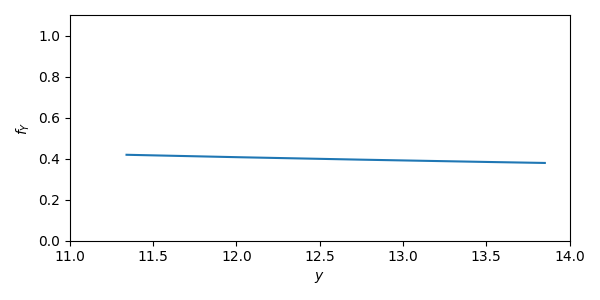
\includegraphics[height=2.3cm]{2.12.png}
\end{figure}
虽然零件半径是均匀分布，但截面积的分布会略微倾向小面积。






\newpage
\section{密度函数的物理意义}

\begin{tcolorbox}
离散变量的分布律的意义是清晰的，每个点代表基本事件的发生概率。
但连续变量的密度函数的意义并不十分清晰，本节讨论密度函数的物理意义，以求能直观地把握这个概念。
\end{tcolorbox}

若有一维无限长细线，总质量为$M$但分布不均匀，已知线密度$\rho \left( l \right) $，$l$为距原点的距离，任取一段$\left[ l_1,l_2 \right] $，该段质量占比为：
\begin{figure}[h]
\centering
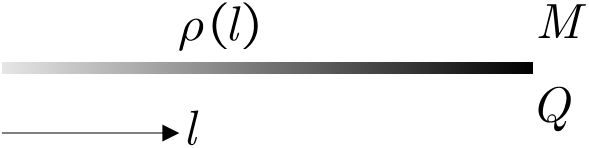
\includegraphics[height=1.2cm]{2.13.png}
\end{figure}
\[
\frac{m}{M}=\int_{l_1}^{l_2}{\frac{\rho \left( l \right)}{M}\cdot dl}
\]

若考虑一维无限长带电细线，总电荷量为$Q$但分布不均匀，已知电密度$\rho \left( l \right) $，任取一段$\left[ l_1,l_2 \right] $，该段电荷占比为：
\[
\frac{q}{Q}=\int_{l_1}^{l_2}{\frac{\rho \left( l \right)}{Q}\cdot dl}
\]

再考虑变速运动，若速度随时间变化且有规律$v=v\left( t \right) $，则在某时段走过的路程占总路程$S$：
\[
\frac{s}{S}=\int_{t_1}^{t_2}{\frac{v\left( t \right)}{S} \cdot dt}
\]

对比概率计算公式：
\[
P\left\{ a<X\leqslant b \right\} =\int_a^b{f\left( x \right) \cdot dx}
\]
容易发现，概率$P\left\{ a<X\leqslant b \right\} $表示了一段范围内某个物理量的占比，密度函数$f\left( x \right) $刻画了该物理量的分布情况。
根据$\rho \left( l \right) $我们可以知道哪里重，根据$v \left( t \right) $我们可以知道哪个时段走得多。
同样道理，根据密度函数，我们可以知道$X$在哪里出现的概率大。
关联到具体事件，我们就可以知道哪些事件容易发生。
所以，我们通常用“占比大”、“出现多”来指代概率大。

~

{\bf 密度函数的物理意义是反映了一个物理量在某个范围内的占比。}
这个“占比”就是概率，而“范围”可以是空间上的一个段，也可以是时间上的一个段。
以质量为例，可以认为密度函数具有量纲$\left[ \mathrm{m}^{-1} \right] $。






\newpage
\section{本章小结}

本章讨论了一维随机变量，将事件和概率进行数学上的抽象，上升为函数，用函数刻画概率，描绘生活中常见的概率的分布规律。

一个变量是否为随机变量主要看它有没有对应的分布函数，而分布函数就看充要条件：
\[
\begin{cases}
	0\leqslant F\left( x \right) \leqslant 1\\
	\underset{x\rightarrow -\infty}{\lim}F\left( x \right) =P\left( \oslash \right) =0\\
	\underset{x\rightarrow +\infty}{\lim}F\left( x \right) =P\left( \varOmega \right) =1\\
\end{cases}
\]
该充要条件是后续一切概念的基础。
根据该条件，我们才定义（或者说推导）了离散变量的分布律和连续变量的密度函数这两个概念。

\begin{table}[h]
\centering
\caption{离散变量和连续变量的对比}
\begin{tabular}{cccc}
    \toprule
     & 符号 & 描述 & 概率、分布函数\\
    \midrule
    离散型 & $X$ & 分布律$p_i$ & $P\left\{ X\leqslant x \right\} =F\left( x \right) =\sum_{x_i\leqslant x}{p_i}$\\
    连续型 & $X$ & 密度函数$f\left( x \right) $ & $P\left\{ X\leqslant x \right\} =F\left( x \right) =\int_{-\infty}^x{f\left( t \right) \cdot dt}$\\
    \bottomrule
\end{tabular}
\end{table}

离散变量有单点概率$P\left\{ X=x_i \right\} =p_i$，也即基本事件的概率。
连续变量没有“单点概率”，$P\left\{ X=x_i \right\} $始终为0，单纯理论上的单点概率为0在现实中并不表示“不可能”，同样，若密度函数在某点为0在现实中也并不表示该点“不可能”，参考一维无限深势阱。
离散变量的分布律也可以看成“密度”，只是我们可以认为
\[
P\left\{ X\leqslant x \right\} =F\left( x \right) =\sum_{x_i\leqslant x}{p_i\cdot \Delta x},   \Delta x=1
\]
于是在计算单点概率时有$P\left\{ X=x_i \right\} =p_i\cdot \Delta x=p_i\cdot 1=p_i$。

本章还讨论了随机变量的函数，特别注意，连续变量的函数是否依然是连续型，取决于$Y=g\left( X \right) $是否为单调。










\chapter{二维随机变量及其分布}

在有两个随机变量的情况下，概率的分布将变得复杂。
本章介绍二维随机变量的相关概念，包括分布函数、分布律和密度函数。
此外，在两个变量相互作用方面，还有边缘分布、条件分布和独立性的概念。

本章要点：
\begin{itemize}
    \item 二维随机变量的概念，以及2大类，离散型和连续型。
    \item 二维随机变量的分布律和密度函数。
    \item 二维随机变量的相互关系，边缘、条件、独立。
\end{itemize}

\newpage
\section{引子}

上一章我们只抽象了一个事件。
本章我们将抽象两个事件。
先考虑一个实际例子。

~

\begin{example}
设甲、乙两人约定在1:00～2:00之间在某处碰头，若有一个先到，等10分钟后如无人则离去，设两人会在1:00～2:00之间任意时刻抵达约定地点，计算两人碰面的概率。
\end{example}

解：

我们从直观感觉出发，首先可以确定，甲、乙两人各自出现在约定地点的概率在1:00～2:00间均匀分布，从图形来看，即下图阴影区的占比。
这是一个典型的几何概率，可得：
\begin{figure}[h]
\centering
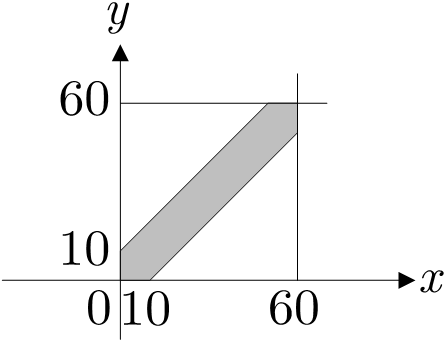
\includegraphics[height=2.4cm]{3.1.png}
\end{figure}
\[
P=1-\frac{2\cdot \left( \frac{1}{2}\cdot 50\cdot 50 \right)}{60\cdot 60}=\frac{11}{36}
\]
虽然结果是对的，但缺乏严密地推理，也不利于推广到任意情况，如甲若偏好来得迟，概率结果会如何等等。

~

本章就是将两个变量的情况加以详细讨论。






\newpage
\section{二维随机变量与分布函数}

本节介绍二维随机变量和分布函数，为之后讨论奠定基础。

本节要点：
\begin{itemize}
    \item 深刻掌握二维随机变量的概念；
    \item 掌握分布函数的概念。
\end{itemize}

%============================================================
\subsection{二维随机变量的概念}

\begin{definition}[二维随机变量]
设随机试验$E$的样本空间$\varOmega $，若$X,Y$均为定义在$\varOmega $上的一维随机变量，则称$\left( X,Y \right) $为{\bf 定义在$\varOmega $上的二维随机变量}，简称{\bf 二维变量}。
\end{definition}

该定义除了简单将两个一维变量进行组合之外，没有任意其他含义，二维变量更多的含义体现在分布函数。

%============================================================
\subsection{分布函数的概念}

\begin{definition}[分布函数]
设二维变量$\left( X,Y \right) $，若对于任意的$X\leqslant x$且$Y\leqslant y$，均有唯一的$P\left\{ X\leqslant x,Y\leqslant y \right\} $与之对应，则称该对应关系为{\bf $\left( X,Y \right) $的分布函数}，也称为{\bf $X$和$Y$的联合分布函数}，记作$F\left( x,y \right) $，即：
\[
F\left( x,y \right) := P\left\{ X\leqslant x,Y\leqslant y \right\} ,\qquad x,y\in \mathbb{R}
\]
\end{definition}

$F\left( x,y \right) $描述了$\left( X,Y \right) $落入平面$\left( -\infty ,x \right] \times \left( -\infty ,y \right] $中的概率。
同一维变量的分布函数，定义隐含了判断一个函数能否被视为分布函数的充要条件：
\[
F\left( x,y \right) \text{是分布函数}\Leftrightarrow \begin{cases}
	0\leqslant F\left( x,y \right) \leqslant 1\\
	\underset{x,y\rightarrow -\infty}{\lim}F\left( x,y \right) =0\\
	\underset{x\rightarrow -\infty}{\lim}F\left( x,y \right) =0\\
	\underset{y\rightarrow -\infty}{\lim}F\left( x,y \right) =0\\
	\underset{x,y\rightarrow +\infty}{\lim}F\left( x,y \right) =1\\
\end{cases}
\]

分布函数的性质：
\begin{itemize}
    \item $F\left( x,y \right) $必单调增，即$x_1<x_2\Rightarrow F\left( x_1,y_0 \right) \leqslant F\left( x_2,y_0 \right) $。
    \item $F\left( x,y \right) $关于点$\left( x,y \right) $右连续。
    \item 落在$\left( x_1,x_2 \right] \times \left( y_1,y_2 \right] $的概率$P\left\{ x_1<X\leqslant x_2,y_1<Y\leqslant y_2 \right\} $为：

	$F\left( x_2,y_2 \right) -F\left( x_1,y_2 \right) -F\left( x_2,y_1 \right) +F\left( x_1,y_1 \right) $
\end{itemize}

总体来讲，$F\left( x,y \right) $呈现了一个东北高、西南低的斜坡。

还需注意$P\left\{ x_1<X\leqslant x_2,y_1<Y\leqslant y_2 \right\} $是事件逻辑和的运算法则，是概率遵循逻辑运算的结果。

%============================================================
\subsection{例}

\begin{example}
若二维变量$\left( X,Y \right) $有分布函数
\[
F\left( x,y \right) =a\left( b+\mathrm{arc}\tan x \right) \left( c+\mathrm{arc}\tan y \right)
\]
计算$P\left\{ X\leqslant 1,Y\leqslant 1 \right\} ,P\left\{ X>1,Y>1 \right\} $。
\end{example}

解：

首先求解具体的分布函数，由分布函数充要条件可得：
\begin{align*}
&\because \begin{cases}
	\underset{x,y\rightarrow +\infty}{\lim}F\left( x,y \right) =a\left( b+\frac{\pi}{2} \right) \left( c+\frac{\pi}{2} \right) =1\\
	\underset{x\rightarrow -\infty}{\lim}F\left( x,y \right) =a\left( b-\frac{\pi}{2} \right) \left( c+\mathrm{arc}\tan y \right) =0\\
	\underset{y\rightarrow -\infty}{\lim}F\left( x,y \right) =a\left( b+\mathrm{arc}\tan x \right) \left( c-\frac{\pi}{2} \right) =0\\
\end{cases}\Rightarrow \begin{cases}
	a=\frac{1}{\pi ^2}\\
	b=\frac{\pi}{2}\\
	c=\frac{\pi}{2}\\
\end{cases} \\
&\therefore F\left( x,y \right) =\frac{1}{\pi ^2}\left( \frac{\pi}{2}+\mathrm{arc}\tan x \right) \left( \frac{\pi}{2}+\mathrm{arc}\tan y \right)
\end{align*}
于是：
\begin{align*}
&P\left\{ X\leqslant 1,Y\leqslant 1 \right\} =F\left( 1,1 \right) =\frac{1}{\pi ^2}\left( \frac{\pi}{2}+\frac{\pi}{4} \right) \left( \frac{\pi}{2}+\frac{\pi}{4} \right) =\frac{9}{16} \\
&P\left\{ X>1,Y>1 \right\} \\
&=P\left\{ 1<X<+\infty ,1<Y<+\infty \right\} \\
&=F\left( +\infty ,+\infty \right) -F\left( 1,+\infty \right) -F\left( +\infty ,1 \right) +F\left( 1,1 \right) \\
&=1-\frac{3}{4}-\frac{3}{4}+\frac{9}{16}=\frac{1}{16}
\end{align*}






\newpage
\section{二维随机变量及其分布规律}

本节介绍二维随机变量及其的分布律。

本节要点：
\begin{itemize}
    \item 掌握二维离散型随机变量的及其分布律的概念；
    \item 掌握二维连续型随机变量的及其密度函数的概念。
\end{itemize}

%============================================================
\subsection{二维离散型随机变量及其分布律的概念}

\begin{definition}[二维离散型随机变量及其分布律]
若二维随机变量$\left( X,Y \right) $的取值为有限个或可列无穷多个，则称$\left( X,Y \right) $为{\bf 二维离散型随机变量}，简称{\bf 二维离散变量}。
设所有可能的取值设为$\left( x_i,y_j \right) ,i=1,2,\cdots ,j=1,2,\cdots $，则对应的概率记作：
\[
P\left\{ X=x_i,Y=y_j \right\} =p_{ij}
\]
称为{\bf 二维离散型随机变量$\left( X,Y \right) $的分布律}，一般可用二维表格罗列。
其中：
\begin{itemize}
    \item $x_i$：纯数学记号，对应事件$A_i$；
    \item $y_i$：纯数学记号，对应事件$B_i$；
    \item $p_{ij}=P\left\{ X=x_i,Y=y_j \right\} =P\left( A_iB_j \right) $：$A_i,B_j$同时发生的概率。
\end{itemize}
\end{definition}

若二维离散变量$\left( X,Y \right) $有分布律$p_{ij}$，则其分布函数为：
\[
F\left( x,y \right) =P\left\{ X\leqslant x,Y\leqslant y \right\} =\sum_{x_i\leqslant x,y_j\leqslant y}{p_{ij}}
\]
由分布函数的充要条件可得$p_{ij}$成为分布律的充要条件：
\[
p_{ij}\text{为分布律}\Leftrightarrow \begin{cases}
	p_{ij}\geqslant 0\\
	\sum_j{\sum_i{p_{ij}}}=1\\
\end{cases}
\]
其中：
\begin{itemize}
    \item $\sum_j{\sum_i{p_{ij}}}$：表示将所有的$p_{ij}$累加起来。
\end{itemize}

\begin{tcolorbox}
再次注意，分布律$p_{i,j}$表示两个事件都发生。
\end{tcolorbox}

%============================================================
\subsection{二维连续型随机变量及其密度函数的概念}

\begin{definition}[二维连续型随机变量及其密度函数]
设二维随机变量$\left( X,Y \right) $及其分布函数$F\left( x,y \right) $，若存在二元可积函数$f\left( x,y \right) \geqslant 0$，对于$\forall x,y$，有：
\[
F\left( x,y \right) =\iint\limits_D{f\left( u,v \right) \cdot d\sigma},\qquad \begin{array}{l}
	d\sigma =dudv\\
	D=\left\{ \left( u,v \right) \middle| u\leqslant x,v\leqslant y \right\}\\
\end{array}
\]
则称$\left( X,Y \right) $为{\bf 二维连续型随机变量}，简称{\bf 二维连续变量}，并称$f\left( x,y \right) $为{\bf 二维连续型随机变量$\left( X,Y \right) $的密度函数}。
\end{definition}

由分布函数的充要条件易得$f\left( x,y \right) $为密度函数的充要条件：
\[
f\left( x,y \right) \text{为密度函数}\Leftrightarrow \begin{cases}
	f\left( x,y \right) \geqslant 0\\
	\iint\limits_{\mathbb{R} \times \mathbb{R}}{f\left( x,y \right) \cdot d\sigma}=1,\quad d\sigma =dxdy\\
\end{cases}
\]
对于任意平面$D$的概率有：
\[
P\left\{ \left( X,Y \right) \in D \right\} =\iint\limits_D{f\left( x,y \right) \cdot d\sigma},\qquad d\sigma =dxdy
\]

\begin{tcolorbox}
同样，密度函数$f\left( x,y \right) $表示两个事件都发生的概率密度。
其次，一个二维变量是否为连续型，看它有没有密度函数，至于变量本身是整个连续还是分段连续并不要紧。
\end{tcolorbox}


\begin{theorem}
设二维连续随机变量$\left( X,Y \right) $有分布函数$F\left( x,y \right) $和密度函数$f\left( x,y \right) $，若$f\left( x,y \right) $在点$\left( x_0,y_0 \right) $处连续，则：
\[
f\left( x_0,y_0 \right) =\frac{\partial ^2F\left( x_0,y_0 \right)}{\partial x\partial y}=\frac{\partial ^2F\left( x_0,y_0 \right)}{\partial y\partial x}
\]
\end{theorem}

可用微积分的二阶混偏相等定理证明，略。

%============================================================
\subsection{例}

\begin{example}
若5个产品中有2个次品，每次抽取一个，取两次，记$X$表示第一次取到次品的个数，$Y$表示第二次取到次品的个数，试求：
\begin{enumerate}
    \item 不放回抽取的情况下，$\left( X,Y \right) $的分布律，
    \item 放回抽取的情况下，$\left( X,Y \right) $的分布律。
\end{enumerate}
\end{example}

解：

由题干可得，$X,Y$取值只可能是0或1，0表示抽到合格品，1表示抽到次品。

1. 不放回抽取的情况下：
\begin{align*}
&P\left\{ X=0,Y=0 \right\} =\frac{3}{5}\cdot \frac{2}{4}=\frac{3}{10} \\
&P\left\{ X=1,Y=0 \right\} =\frac{2}{5}\cdot \frac{3}{4}=\frac{3}{10} \\
&P\left\{ X=0,Y=1 \right\} =\frac{3}{5}\cdot \frac{2}{4}=\frac{3}{10} \\
&P\left\{ X=1,Y=1 \right\} =\frac{2}{5}\cdot \frac{1}{4}=\frac{1}{10}
\end{align*}

2. 放回抽取的情况下：
\begin{align*}
&P\left\{ X=0,Y=0 \right\} =\frac{3}{5}\cdot \frac{3}{5}=\frac{9}{25} \\
&P\left\{ X=1,Y=0 \right\} =\frac{2}{5}\cdot \frac{3}{5}=\frac{6}{25} \\
&P\left\{ X=0,Y=1 \right\} =\frac{3}{5}\cdot \frac{2}{5}=\frac{6}{25} \\
&P\left\{ X=1,Y=1 \right\} =\frac{2}{5}\cdot \frac{2}{5}=\frac{4}{25}
\end{align*}

~

\begin{example}
若二维连续随机变量$\left( X,Y \right) $有密度函数
\[
f\left( x,y \right) =\begin{cases}
	ke^{-x},&		y\in \left( 0,x \right)\\
	0,&		y\notin \left( 0,x \right)\\
\end{cases}
\]
计算分布函数和$P\left\{ X+Y<2 \right\} $。
\end{example}

解：

首先得计算具体的密度函数，由密度函数的充要条件得：
\begin{align*}
&\because \iint\limits_D{f\left( x,y \right) \cdot d\sigma}=1,\quad D=\left\{ \left( x,y \right) \middle| x>0,0<y<x \right\} \\
&\because \iint\limits_D{ke^{-x}\cdot d\sigma}=\int_0^{+\infty}{dx}\int_0^x{ke^{-x}\cdot dy}=\int_0^{+\infty}{kxe^{-x}\cdot dx}=k \\
&\therefore k=1 \\
&\therefore f\left( x,y \right) =\begin{cases}
	e^{-x},&		y\in \left( 0,x \right)\\
	0&		y\notin \left( 0,x \right)\\
\end{cases}
\end{align*}
使用了部分积分法$\int{xe^xdx}=\int{xd\left( e^x \right)}=xe^x-\int{e^xdx}$。

\begin{figure}[ht]
	\centering
	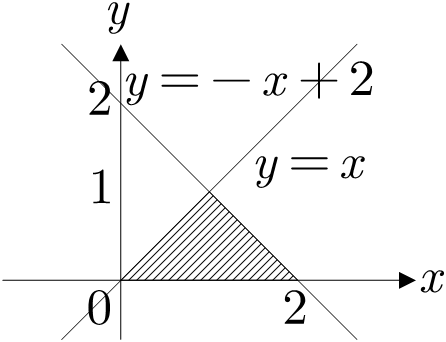
\includegraphics[height=2.5cm]{3.2.png}
	\end{figure}

$P\left\{ X+Y<2 \right\} $的区域为$\left\{ \left( x,y \right) \middle| x\in \left[ 0,2 \right] ,y\in \left[ 0,\min \left\{ x,-x+2 \right\} \right] \right\} $
。由于积分区域是凸区域，所以积分结果和次序无关：
\[
P\left\{ \left( X,Y \right) \in D \right\} =\iint\limits_D{e^{-x}\cdot d\sigma}=\int_0^1{dy}\int_y^{2-y}{e^{-x}\cdot dx}=1-2e^{-1}+e^{-2}
\]






\newpage
\section{常见的密度函数}

本节介绍几个常见的二维连续变量的密度函数。

本节要点：
\begin{itemize}
    \item 理解2个常见的密度函数及其应用场景；
    \item 学会用这2个密度函数考察实际问题。
\end{itemize}

%============================================================
\subsection{二维均匀分布}

{\bf 二维均匀分布}，记作$U\left( D \right) $，描述了最简单的分布：
\[
f\left( x,y \right) =\begin{cases}
	\frac{1}{S_D},&		\left( x,y \right) \in D\\
	0,&		\left( x,y \right) \notin D\\
\end{cases}
\]
其中：
\begin{itemize}
    \item $D$：表示变量$\left( X,Y \right) $的取值区域；
    \item $S_D$：表示$D$的面积。
\end{itemize}

\begin{tcolorbox}
二维均匀分布是一维均匀分布的扩展，和几何概型联系紧密。
\end{tcolorbox}

%============================================================
\subsection{二维正态分布}
{\bf 二维正态分布}，记作$N\left( \mu _1,\mu _2,{\sigma _1}^2,{\sigma _2}^2,\rho \right) $：

\begin{figure}[h]
\centering
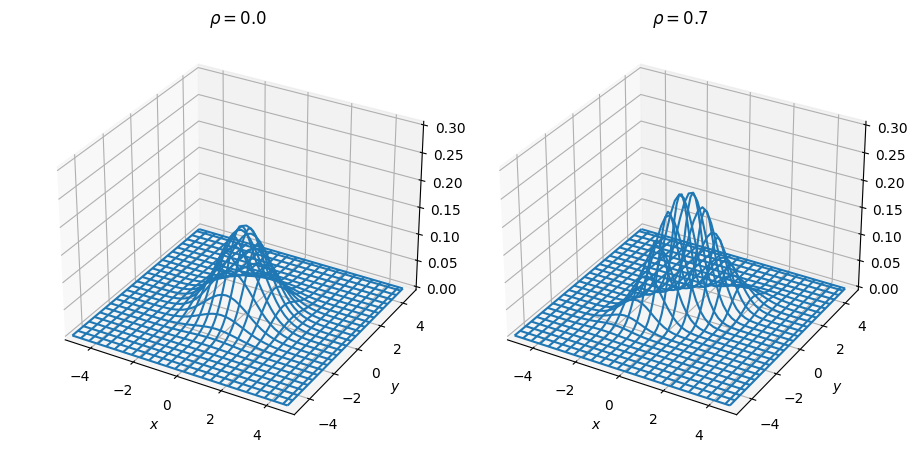
\includegraphics[height=5.5cm]{3.3.png}
\caption{二维正态分布}
\end{figure}

\begin{align*}
&f\left( x,y \right) =\frac{1}{2\pi \sigma _1\sigma _2\sqrt{1-\rho ^2}}e^{-\frac{1}{2\left( 1-\rho ^2 \right)}\left[ \frac{\left( x-\mu _1 \right) ^2}{{\sigma _1}^2}-2\rho \frac{\left( x-\mu _1 \right) \left( y-\mu _2 \right)}{\sigma _1\sigma _2}+\frac{\left( y-\mu _2 \right) ^2}{{\sigma _2}^2} \right]} \\
&\mu _1,\mu _2\in \mathbb{R}\qquad \sigma _1,\sigma _2>0\qquad \rho \in \left( -1,1 \right)
\end{align*}

特点：
\begin{itemize}
    \item $f\left( x,y \right) $是三维空间的一个钟形曲面，出现在\textit{xy}平面上方；
    \item 曲面$f\left( x,y \right) $关于两个平面$x=\mu _1$和$y=\mu _2$对称；
    \item $\mu _1,\mu _2,\sigma _1,\sigma _2$：描述各自的中心点和平坦度，与一维正态分布同理；
    \item $\rho $：$X$和$Y$的相关系数$\rho _{XY}$，后面介绍；
    \item \textit{xy}平面是$f\left( x,y \right) $的水平渐进面。
\end{itemize}






\newpage
\section{密度函数的物理意义}

若有二维无限大平面，总质量$M$但分布不均匀，已知面密度$\rho \left( x,y \right) $，$x,y$为距原点的坐标距离，则任意区域$D$的质量占比：
\begin{figure}[h]
    \begin{minipage}{0.48\linewidth}
    \centerline{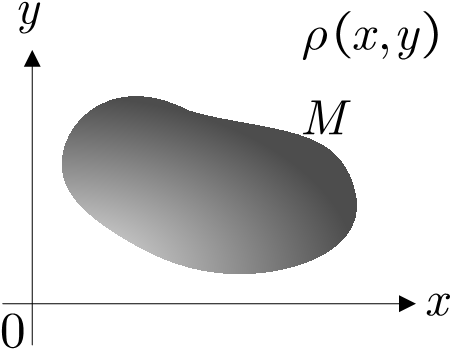
\includegraphics[width=3.5cm]{3.4.png}}
    \end{minipage}
\hfill
    \begin{minipage}{0.48\linewidth}
    \begin{align*}
    &\frac{m}{M}=\iint\limits_D{\frac{\rho \left( x,y \right)}{M}\cdot d\sigma} \\
    &d\sigma =dxdy
    \end{align*}
    \end{minipage}
\end{figure}

对比概率计算公式：
\[
P\left\{ \left( X,Y \right) \in D \right\} =\iint\limits_D{f\left( x,y \right) \cdot d\sigma}
\]

~

{\bf 二维变量的密度函数的物理意义是反映了某个物理量在一个二维的范围$D$内的占比，若以质量为例，则可认为具有量纲$\left[ \mathrm{m}^{-2} \right] $。}
二维平面上的点$\left( x,y \right) $对应到概率论就是二维变量$\left( X,Y \right) $，关联到具体事件就是表示两个事件同时发生，通过密度函数我们就可以知道哪些“合并事件”容易发生。

~

特别注意，如果平面$D$退化成线$L$，则：
\[
P\left\{ \left( X,Y \right) \in L \right\} =\iint\limits_L{f\left( x,y \right) \cdot d\sigma}=0
\]
可认为平面上任何“线质量”都是0。






\newpage
\section{关于二维随机变量的其他概念}

本节在函数的框架下考察二维变量的相互关系，包括边缘、条件、独立。
其中，边缘是后两个概念的基础。

本节要点：
\begin{itemize}
    \item 掌握边缘分布的概念；
    \item 掌握条件分布的概念；
    \item 深刻掌握独立性的概念。
\end{itemize}

%============================================================
\subsection{二维随机变量的边缘分布}

\begin{definition}[边缘分布函数]
设有二维变量$\left( X,Y \right) $，则称$X$和$Y$的分布函数为{\bf $\left( X,Y \right) $关于$X$和$Y$的边缘分布函数}，记作$F_X\left( x \right) $和$F_Y\left( y \right) $，且有：
\begin{align*}
&F_X\left( x \right) :=\underset{y\rightarrow +\infty}{\lim}F\left( x,y \right) \\
&F_Y\left( y \right) :=\underset{x\rightarrow +\infty}{\lim}F\left( x,y \right)
\end{align*}
\end{definition}

\begin{definition}[边缘分布率]
设有二维离散变量$\left( X,Y \right) $，则称$X$和$Y$的分布律为{\bf $\left( X,Y \right) $关于$X$和$Y$的边缘分布律}，分别记作$P\left\{ X=x_i \right\} $和$P\left\{ Y=y_i \right\} $，也可记作$p_{i\cdot}$和$p_{\cdot j}$，即：
\begin{align*}
&P\left\{ X=x_i \right\} =p_{i\cdot}:=\sum_j{p_{ij}} \\
&P\left\{ Y=y_j \right\} =p_{\cdot j}:=\sum_i{p_{ij}}
\end{align*}
其中：
\begin{itemize}
    \item $p_{i\cdot}:=\sum_j{p_{ij}}$：表示固定$i$时，将所有$j$累加，即$X$的边缘分布是对表格进行纵向求和得到；
    \item $p_{\cdot j}:=\sum_i{p_{ij}}$：表示固定$j$时，将所有$i$累加，即$Y$的边缘分布是对表格进行横向求和得到。
\end{itemize}
\end{definition}

\begin{figure}[h]
\centering
\centerline{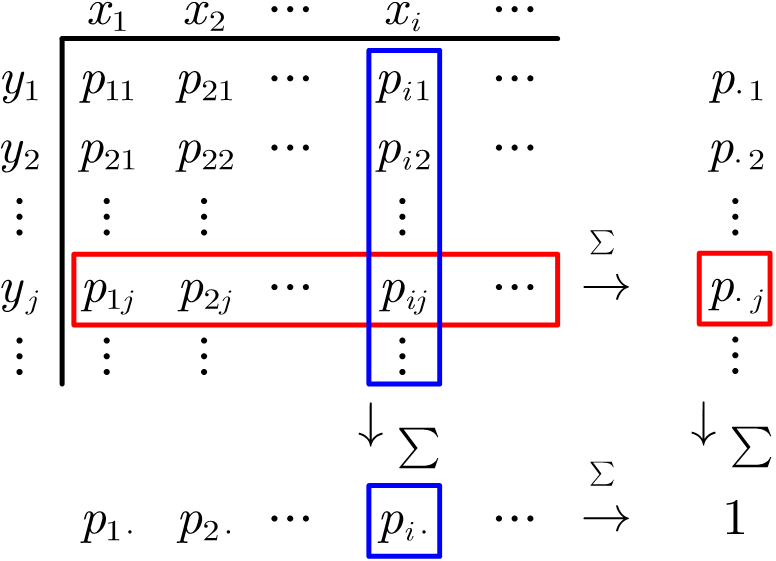
\includegraphics[width=5cm]{3.5.png}}
\end{figure}

\begin{definition}[边缘密度函数]
设有二维连续变量$\left( X,Y \right) $，则称$X$和$Y$的密度函数为{\bf $\left( X,Y \right) $关于$X$和$Y$的边缘密度函数}，分别记作$f_X\left( x \right) $和$f_Y\left( y \right) $，即：
\begin{align*}
&f_X\left( x \right) :=\int_{-\infty}^{+\infty}{f\left( x,y \right) \cdot dy} \\
&f_Y\left( y \right) :=\int_{-\infty}^{+\infty}{f\left( x,y \right) \cdot dx}
\end{align*}
\end{definition}

边缘分布强调的是只考虑一个因素，当考虑$X$方面的概率时，我们需要排除$Y$的不确定性，一种本能的、直观的做法就是将所有$Y$的概率累加。
在二维离散变量的分布律表格中，边缘分布一般作为按行求和和按列求和书写在表格左边和下边，故称“边缘分布”。
由于在计算过程中损失了$Y$的分布细节，所以知道边缘分布并不能还原出$X$和$Y$的联合分布。
从原理上来讲，一切变量$X$的分布都是某个“不知名变量”的边缘分布，对于不同的$Y$可能有不同的边缘分布，当然也有可能是相同的。
最后，边缘密度函数就是计算二重积分时的“第一个切片”。

%============================================================
% 二维随机变量的条件分布
%============================================================
\subsection{二维随机变量的条件分布}

\begin{tcolorbox}
上面我们讨论了“不考虑$Y$”时$X$的概率。
现在，我们考虑$Y$维度上发生某个事件的时候$X$的概率。
\end{tcolorbox}

\begin{definition}[条件分布函数]
设二维变量$\left( X,Y \right) $，当$Y=y_0$时，对于$\forall \varepsilon >0$，若存在极限
\[
\underset{\varepsilon \rightarrow 0^+}{\lim}\frac{P\left\{ X\leqslant x,y_0-\varepsilon <Y\leqslant y_0+\varepsilon \right\}}{P\left\{ y_0-\varepsilon <Y\leqslant y_0+\varepsilon \right\}}
\]
则称此极限为在$\left\{ Y=y_0 \right\} $发生时的{\bf $X$的条件分布函数}，记作$F_{X|Y}\left( x \middle| y_0 \right) $，同样可定义在$\left\{ X=x_0 \right\} $发生时的{\bf $Y$的条件分布函数}，记作$F_{Y|X}\left( y \middle| x_0 \right) $，即：
\begin{align*}
    &F_{X|Y}\left( x \middle| y_0 \right) :=\underset{\varepsilon \rightarrow 0^+}{\lim}\frac{P\left\{ X\leqslant x,y_0-\varepsilon <Y\leqslant y_0+\varepsilon \right\}}{P\left\{ y_0-\varepsilon <Y\leqslant y_0+\varepsilon \right\}} \\
    &F_{Y|X}\left( y \middle| x_0 \right) :=\underset{\varepsilon \rightarrow 0^+}{\lim}\frac{P\left\{ Y\leqslant y,x_0-\varepsilon <X\leqslant x_0+\varepsilon \right\}}{P\left\{ x_0-\varepsilon <X\leqslant x_0+\varepsilon \right\}}
\end{align*}
\end{definition}

\begin{definition}[条件分布律]
设二维离散变量$\left( X,Y \right) $有分布律$p_{ij}$，若已知$Y$的边缘分布有$p_{\cdot j}$，当取值$Y=y_{j_0}$时，称$\frac{p_{ij_0}}{p_{\cdot j_0}}$为在条件$\left\{ Y=y_{j_0} \right\} $下的{\bf $X$的条件分布律}，记作$P\left\{ X=x_i \middle| Y=y_{j_0} \right\} $，同样可定义在条件$\left\{ X=x_{i_0} \right\} $下的{\bf $Y$的条件分布律}：
\begin{align*}
&P\left\{ X=x_i \middle| Y=y_{j_0} \right\} :=\frac{P\left\{ X=x_i,Y=y_{j_0} \right\}}{P\left\{ Y=y_{j_0} \right\}}=\frac{p_{ij_0}}{p_{\cdot j_0}} \\
&P\left\{ Y=y_j \middle| X=x_{i_0} \right\} :=\frac{P\left\{ Y=y_j,X=x_{i_0} \right\}}{P\left\{ X=x_{i_0} \right\}}=\frac{p_{i_0j}}{p_{i_0\cdot}}
\end{align*}
\end{definition}

\begin{figure}[h]
\centering
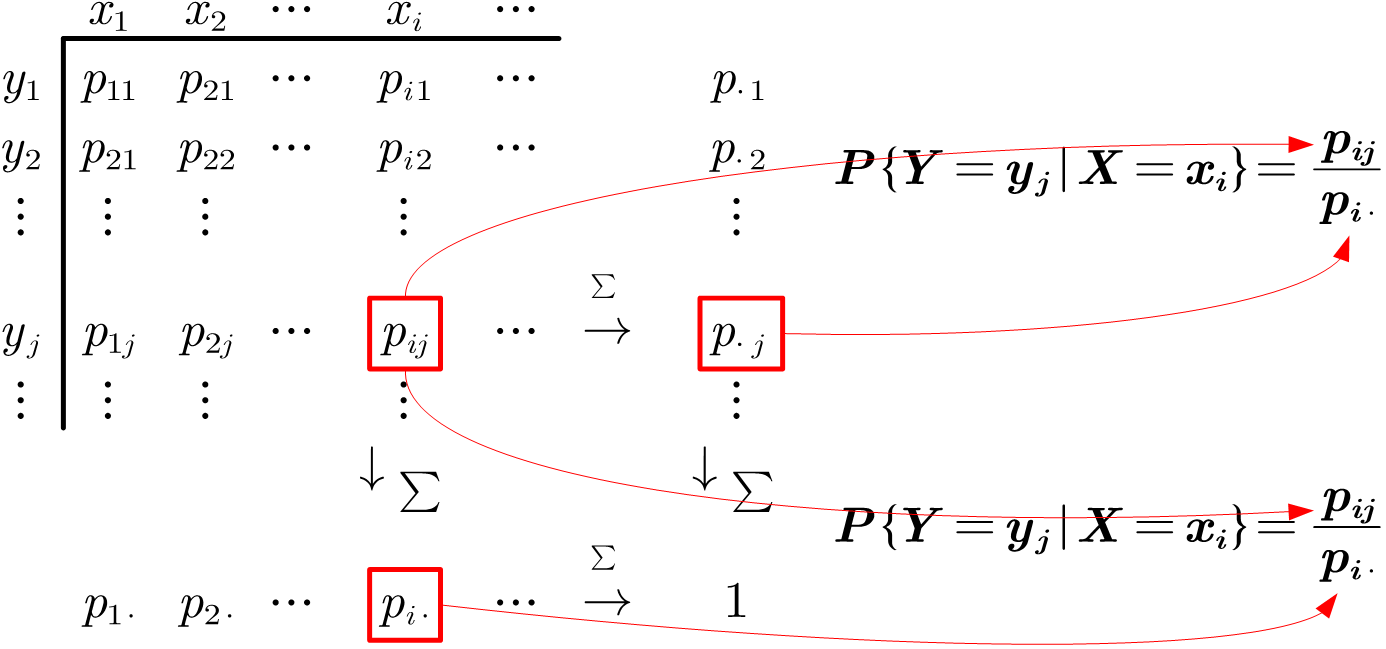
\includegraphics[height=4.5cm]{3.6.png}
\end{figure}

\begin{definition}[{条件密度函数}]
设二维连续变量$\left( X,Y \right) $有密度函数$f\left( x,y \right) $，若已知$\left( X,Y \right) $关于$X$和$Y$的边缘密度函数$f_X\left( x \right) $和$f_Y\left( y \right) $，则可定义在条件$Y=y_0$下的{\bf $X$的条件密度函数}和在条件$X=x_0$下的{\bf $Y$的条件密度函数}：
\begin{align*}
&f_{X|Y}\left( x \middle| y_0 \right) :=\frac{f\left( x,y_0 \right)}{f_Y\left( y_0 \right)}=\frac{f\left( x,y_0 \right)}{\int_{-\infty}^{+\infty}{f\left( x,y_0 \right) \cdot dx}} \\
&f_{Y|X}\left( y \middle| x_0 \right) :=\frac{f\left( x_0,y \right)}{f_X\left( x_0 \right)}=\frac{f\left( x_0,y \right)}{\int_{-\infty}^{+\infty}{f\left( x_0,y \right) \cdot dy}}
\end{align*}
\end{definition}

二维变量条件分布中的“条件”一词是指“另一个变量边缘分布概率”。
通过条件分布，我们可以了解一个变量如何影响另一个变量。

条件分布律和条件密度函数跟条件概率定义相仿：
\begin{align*}
&P\left\{ X=x_i \middle| Y=y_j \right\} :=\frac{p_{ij}}{p_{\cdot j}} \\
&f_{X|Y}\left( x \middle| y \right) :=\frac{f\left( x,y \right)}{f_Y\left( y \right)} \\
&P\left( B \middle| A \right) :=\frac{P\left( AB \right)}{P\left( A \right)}
\end{align*}

\begin{tcolorbox}
由于基本事件 和 分别构成完备组，所以条件分布还能引申出相应的全概率公式和贝叶斯公式，本笔记略。
\end{tcolorbox}

%============================================================
\subsection{二维随机变量的独立性}

\begin{definition}[相互独立]
设二维随机变量$\left( X,Y \right) $有分布函数$F\left( x,y \right) $，若已知$X$和$Y$的边缘分布函数为$F_X\left( x \right) $和$F_Y\left( y \right) $，若$\forall x,y\in \mathbb{R} $，有
\[
F\left( x,y \right) =F_X\left( x \right) \cdot F_Y\left( y \right)
\]
则称{\bf $X$和$Y$相互独立}。
\end{definition}

独立性也是建立在边缘分布的基础上。

\begin{theorem}
设二维离散变量$\left( X,Y \right) $有分布律$p_{ij}$，若已知$X$和$Y$的边缘分布有$p_{i\cdot},p_{\cdot j}$，则$X$和$Y$相互独立的充要条件是$\forall i,j$有：
\[
p_{ij}=p_{i\cdot}\cdot p_{\cdot j}
\]
\end{theorem}

\begin{figure}[h]
\centering
\centerline{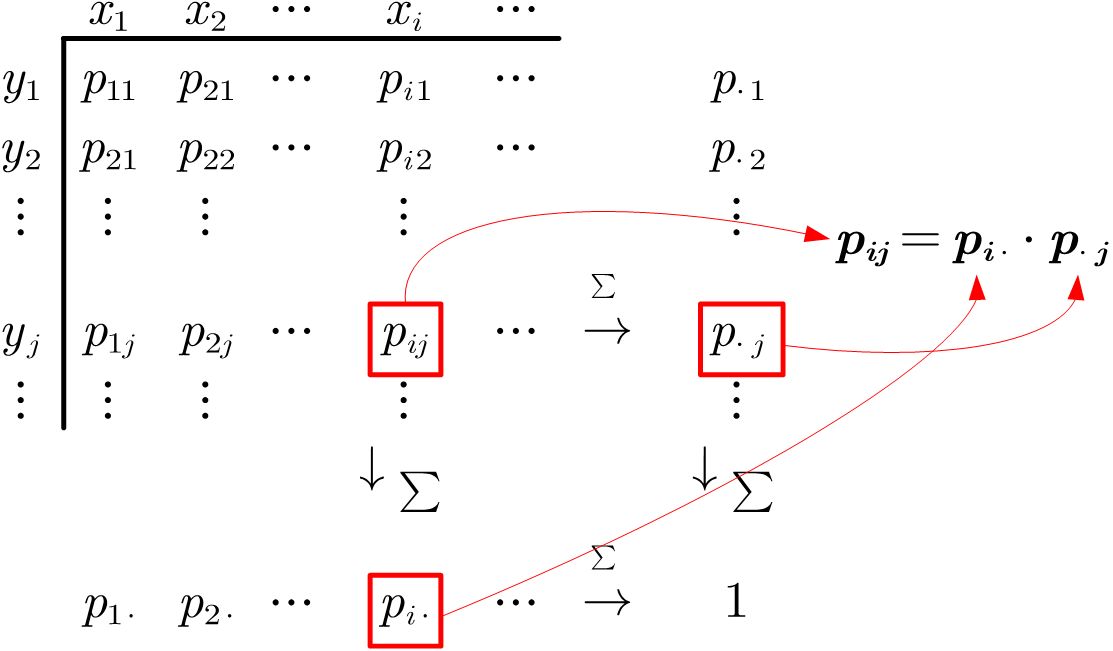
\includegraphics[width=7cm]{3.7.png}}
\end{figure}

\begin{tcolorbox}
$\left( X,Y \right) $的独立性可以和事件独立性概念中的$P\left( AB \right) =P\left( A \right) P\left( B \right) $相互印证学习。
\end{tcolorbox}

\begin{theorem}
设二维连续变量$\left( X,Y \right) $有密度函数$f\left( x,y \right) $，若已知$X$和$Y$的边缘密度函数$f_X\left( x \right) $和$f_Y\left( y \right) $，则$X$和$Y$相互独立的充要条件是对几乎所有点$\left( x,y \right) $有：
\[
f\left( x,y \right) =f_X\left( x \right) \cdot f_Y\left( y \right)
\]
\end{theorem}

由于$f\left( x,y \right) $允许出现有限个不连续点，所以定理中没有要求所有点，而是去除了这些有限个不连续点。

\begin{theorem}
若$X$和$Y$相互独立，则它们在各自任意事件上也相互独立，即：
\[
P\left\{ X\in L_1,Y\in L_2 \right\} =P\left\{ X\in L_1 \right\} \cdot P\left\{ Y\in L_2 \right\}
\]
\end{theorem}

\begin{theorem}
若$X$和$Y$相互独立，且$g\left( x \right) ,h\left( x \right) $是连续函数，则随机变量$g\left( x \right) $和$h\left( x \right) $也相互独立。
\end{theorem}

结合第一章中的独立性讨论，通常我们也不会用定义判断两个变量是否独立，而是从事实角度出发讨论二维分布规律。
通常我们可以较容易地得知各自的边缘分布和较容易地判断出它们是独立的，于是通过独立性的公式，我们就可以计算它们的联合分布规律。
若已知分布函数，则可以用定义判定：
\[
F\left( x,y \right) =F_X\left( x \right) \cdot F_Y\left( y \right)
\]
若已知分布律或密度函数，则可以用定理判断：
\begin{align*}
&p_{ij}=p_{i\cdot}\cdot p_{\cdot j} \\
&f\left( x,y \right) =f_X\left( x \right) \cdot f_Y\left( y \right)
\end{align*}
直观来讲，独立表示$X$的条件分布与$Y$的具体取值无关。

\begin{tcolorbox}
独立性是一个很强的约束，逻辑上要求两者没有任何关系，后面会提到一个叫相关性的概念，表示两者的线性关系，较独立性没有那么强的约束性。
\end{tcolorbox}

%============================================================
\subsection{二维正态分布的讨论}

正态分布有很多特别的性质，这里特别概括二维情况下的正态分布的一些性质。

~

{\bf 关于边缘分布}

\begin{theorem}
若有二维正态分布$\left( X,Y \right) \sim N\left( \mu _1,\mu _2,{\sigma _1}^2,{\sigma _2}^2,\rho \right) $，则必有边缘分布$X\sim N\left( \mu _1,{\sigma _1}^2 \right) ,Y\sim N\left( \mu _2,{\sigma _2}^2 \right) $。
\end{theorem}

该定理说明：
\begin{itemize}
    \item 二维正态分布的边缘分布依然为正态分布；
    \item 各自的分布只与各自参数有关，与$\rho $无关；
    \item 反过来，任意两个边缘正态分布可以根据不同的$\rho $组合出无穷多个二维正态分布。
\end{itemize}

~

{\bf 关于条件分布}

\begin{theorem}
若有二维正态分布$\left( X,Y \right) \sim N\left( \mu _1,\mu _2,{\sigma _1}^2,{\sigma _2}^2,\rho \right) $，则各自的条件分布依然为正态分布，即：
\begin{align*}
&X\sim N\left( \mu _1+\rho \frac{\sigma _1}{\sigma _2}\left( y-\mu _2 \right) ,{\sigma _1}^2\left( 1-\rho \right) \right) \\
&Y\sim N\left( \mu _2+\rho \frac{\sigma _2}{\sigma _1}\left( x-\mu _1 \right) ,{\sigma _2}^2\left( 1-\rho \right) \right)
\end{align*}
\end{theorem}

该定理说明：
\begin{itemize}
    \item 二维正态分布的条件分布依然为正态分布；
    \item 各自的分布不但与各自参数有关，而且与对方参数和$\rho $（$X,Y$之间的相关程度）有关。
\end{itemize}

~

{\bf 关于独立性}

\begin{theorem}
若二维变量服从正态分布$\left( X,Y \right) \sim N\left( \mu _1,\mu _2,{\sigma _1}^2,{\sigma _2}^2,\rho \right) $，则有$X$和$Y$相互独立$\Leftrightarrow \rho =0$。
\end{theorem}

\begin{theorem}
若两个一维变量各自服从正态分布$X\sim N\left( \mu _1,{\sigma _1}^2 \right) ,Y\sim N\left( \mu _2,{\sigma _2}^2 \right) $，且相互独立，则它们构成的二维变量也服从正态分布，且有$\left( X,Y \right) \sim N\left( \mu _1,\mu _2,{\sigma _1}^2,{\sigma _2}^2,0 \right) $。
\end{theorem}

%============================================================
\subsection{例}

\begin{example}
若二维变量$\left( X,Y \right) $的分布函数为
\[
F\left( x,y \right) =\frac{1}{\pi ^2}\left( \frac{\pi}{2}+\mathrm{arc}\tan x \right) \left( \frac{\pi}{2}+\mathrm{arc}\tan y \right)
\]
试讨论$X,Y$的独立性。
\end{example}

答：

由边缘分布的定义易得：
\begin{align*}
F_X\left( x \right) &=\underset{y\rightarrow +\infty}{\lim}F\left( x,y \right) =\underset{y\rightarrow +\infty}{\lim}\frac{1}{\pi ^2}\left( \frac{\pi}{2}+\mathrm{arc}\tan x \right) \left( \frac{\pi}{2}+\mathrm{arc}\tan y \right) \\
&=\frac{1}{\pi}\left( \frac{\pi}{2}+\mathrm{arc}\tan x \right) \\
F_Y\left( y \right) &=\underset{x\rightarrow +\infty}{\lim}F\left( x,y \right) =\underset{x\rightarrow +\infty}{\lim}\frac{1}{\pi ^2}\left( \frac{\pi}{2}+\mathrm{arc}\tan x \right) \left( \frac{\pi}{2}+\mathrm{arc}\tan y \right) \\
&=\frac{1}{\pi}\left( \frac{\pi}{2}+\mathrm{arc}\tan y \right)
\end{align*}
可见$X,Y$相互独立。

~

\begin{example}
甲、乙两人约定在1:00～2:00之间在某处碰头，若有一个先到，等10分钟后如无人则离去，设两人会在1:00～2:00之间任意时刻抵达约定地点，计算两人碰面的概率。
\end{example}

答：

该题是本章引子中的题目，当时用几何分布进行直观分析，这里使用本章的知识重新分析。首先可以确定，甲、乙两人各自出现在约定地点的概率在1:00～2:00间均匀分布，即：
\begin{align*}
&X\sim U\left[ 0,60 \right] ,Y\sim U\left[ 0,60 \right] \\
&f\left( x \right) =\begin{cases}
	\frac{1}{60},&		x\in \left[ 0,60 \right]\\
	0,&		x\notin \left[ 0,60 \right]\\
\end{cases}
\end{align*}
由于两人事先并无沟通，抵达时间也是各凭喜好，所以他们是独立的，于是：
\[
f\left( x,y \right) =f\left( x \right) \cdot f\left( y \right) =\begin{cases}
	\frac{1}{3600},&		x,y\in \left[ 0,60 \right]\\
	0,&		x,y\notin \left[ 0,60 \right]\\
\end{cases}
\]
两人能碰面的概率可表示为$P\left\{ \left| X-Y \right|\leqslant 10 \right\} $，图形表示如下。
阴影部分积分区域较为复杂，但白色区域较为简单，积分区域$D$变成：
\begin{figure}[h]
\centering
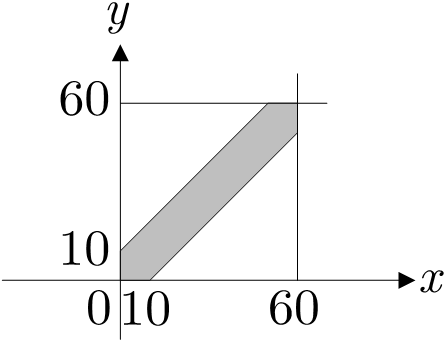
\includegraphics[height=2.4cm]{3.1.png}
\end{figure}
\begin{align*}
&D_1=\left\{ \left( x,y \right) \middle| 10\leqslant x\leqslant 60,0\leqslant y\leqslant x-10 \right\} \\
&D_2=\left\{ \left( x,y \right) \middle| 10\leqslant y\leqslant 60,0\leqslant x\leqslant y-10 \right\} \\
&D=D_1+D_2=2D_1
\end{align*}
计算：
\begin{align*}
P\left\{ \left| X-Y \right|\leqslant 10 \right\} &=1-\iint\limits_D{f\left( x,y \right) \cdot d\sigma}=1-2\int_{10}^{60}{dx}\int_0^{x-10}{\frac{1}{3600}\cdot dy} \\
&=1-\frac{2}{3600}\cdot \left( \left. \frac{1}{2}x^2-10x \right|_{10}^{60} \right) \\
&=\frac{11}{36}
\end{align*}
最终可得他们相遇的概率为$11/36$。






\newpage
\section{边缘分布和条件分布的物理意义}

本节讨论边缘分布和条件分布的物理意义，以加深对这两个概念的认识。

%============================================================
\subsection{边缘分布的物理意义}

从边缘分布的定义公式考虑，取值$X=x_0$时，$X$的边缘分布：
\[
f_X\left( x_0 \right) =\int_{-\infty}^{+\infty}{f\left( x_0,y \right) \cdot dy}
\]
$f_X\left( x_0 \right) $的值是将面分布$f\left( x,y \right) $的值沿直线$x=x_0$加起来，最终形成线分布$f_X\left( x \right) $。
$f_X\left( x \right) $具有量纲$\left[ \mathrm{m}^{-1} \right] $，如下图。
\begin{figure}[h]
\centering
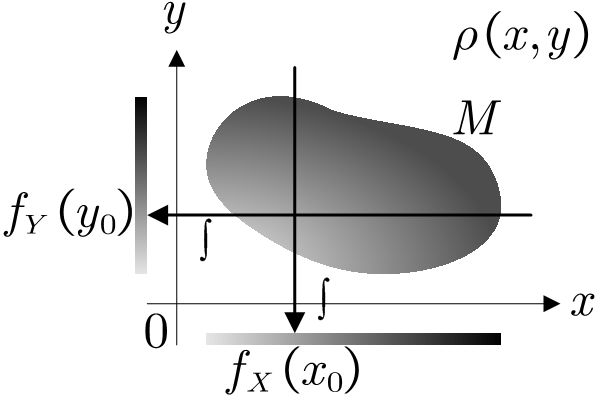
\includegraphics[height=3cm]{3.8.png}
\end{figure}

%============================================================
\subsection{条件分布的物理意义}

设条件$Y=y_0$，从条件分布的定义公式
\[
f_{X|Y}\left( x \middle| y_0 \right) =\frac{f\left( x,y_0 \right)}{f_Y\left( y_0 \right)}
\]
考虑$f_{X|Y}\left( x \middle| y_0 \right) $的值的计算过程：

\begin{enumerate}
    \item 将面分布$f\left( x,y \right) $的值沿直线$y=y_0$抽取出来形成线分布$f\left( x,y_0 \right) $，但此时还是具备同样量纲$\left[ \mathrm{m}^{-2} \right] $，而且$f\left( x,y_0 \right) $并不归一化，即$\int{f\left( x,y_0 \right) dx}\ne 1$，并不能反映线分布的真实状态；
    \item 将该线分布$f\left( x,y_0 \right) $对边缘分布$f_Y\left( y_0 \right) $归一化，得到$f_{X|Y}\left( x_0 \middle| y_0 \right) $，此时具有量纲$\left[ \mathrm{m}^{-1} \right] $，而且反映了线分布的真实状态。
\end{enumerate}
\begin{figure}[h]
\centering
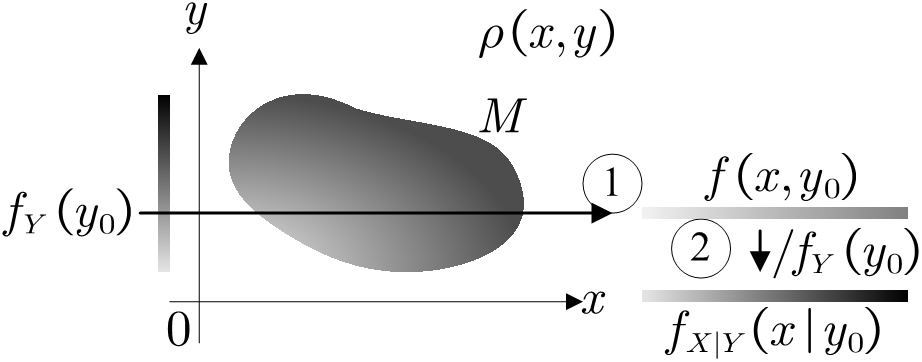
\includegraphics[height=2.5cm]{3.9.png}
\end{figure}
由于$f_Y\left( y_0 \right) <1$，所以：
\[
f_{X|Y}\left( x \middle| y_0 \right) >f\left( x,y_0 \right)
\]
边缘分布是将一个维度上累计，在另一个维度上体现的分布。
条件分布则侧重于抽取“一条”，看这条上的分布。






\newpage
\section{独立性的几何意义}

关于独立性更多意义的讨论见“教材\cite{book1}”的P116～117，本节以二维正态分布讨论独立性的几何意义，以加深认识。

~

二维正态分布$N\left( \mu _1,\mu _2,{\sigma _1}^2,{\sigma _2}^2,\rho \right) $如下：
\[
f\left( x,y \right) =\frac{1}{2\pi \sigma _1\sigma _2\sqrt{1-\rho ^2}}e^{-\frac{1}{2\left( 1-\rho ^2 \right)}\left[ \frac{\left( x-\mu _1 \right) ^2}{{\sigma _1}^2}-2\rho \frac{\left( x-\mu _1 \right) \left( y-\mu _2 \right)}{\sigma _1\sigma _2}+\frac{\left( y-\mu _2 \right) ^2}{{\sigma _2}^2} \right]}
\]
为简化讨论，我们令$\mu _1=\mu _2=0,\sigma _1=\sigma _2=1$。

当$X,Y$独立时，有$\rho =0$，于是：
\[
f\left( x,y \right) =\frac{1}{2\pi}e^{-\frac{x^2+y^2}{2}}
\]
考察$X$的条件分布：
\begin{align*}
f_{X|Y}\left( x \middle| y_0 \right) =\frac{f\left( x,y_0 \right)}{f_Y\left( y_0 \right)}=\frac{\frac{1}{2\pi}e^{-\frac{x^2+{y_0}^2}{2}}}{\int_{-\infty}^{+\infty}{\frac{1}{2\pi}e^{-\frac{x^2+{y_0}^2}{2}}\cdot dx}}=\frac{\frac{1}{2\pi}e^{-\frac{x^2+{y_0}^2}{2}}}{\frac{e^{-\frac{{y_0}^2}{2}}}{2\pi}}=\frac{1}{2\pi}e^{-\frac{x^2}{2}}
\end{align*}
可见$X$的条件分布与$Y$的取值无关，也即无论$Y$取何值，$f\left( x,y_0 \right) $经$f_Y\left( y_0 \right) $归一化后与$Y$无关。
反映在图形上，将曲面$f\left( x,y \right) $沿任意垂直于{\it y}轴的平面进行切片，得到曲线$f\left( x,y_0 \right) $，该曲线是一个“类似”标准分布，只是幅值有不同程度的压缩，但经$f_Y\left( y_0 \right) $归一化后，所有的曲线都相同，如下左图。
但如下右图，$\rho \ne 0$，沿垂直于{\it y}轴的平面切片得到的曲线经$f_Y\left( y_0 \right) $归一化后，虽然形态一样，但沿{\it x}轴有不同程度的位移，表现为不独立。

\begin{figure}[h]
\centering
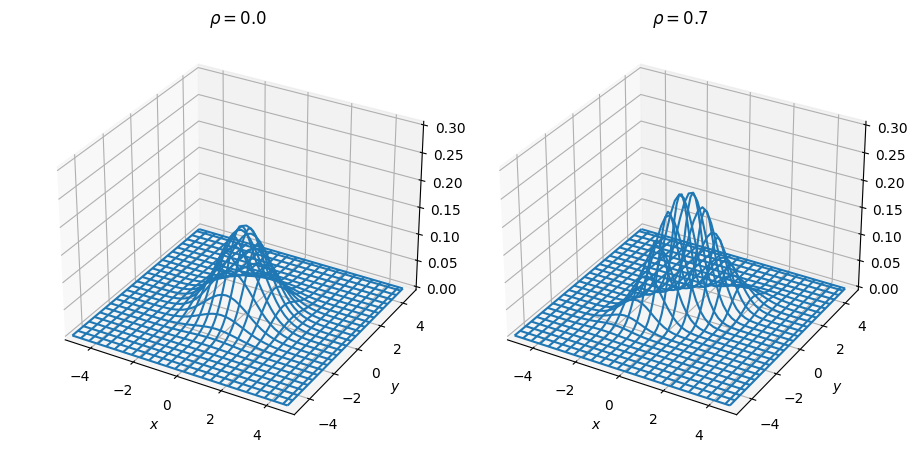
\includegraphics[height=5.5cm]{3.3.png}
\end{figure}

\begin{tcolorbox}
$X$和$Y$独立在几何上的表现，可简单归结为，切片经相应的归一化后的形状与切片位置无关。
\end{tcolorbox}






\newpage
\section{二维随机变量函数的分布}

本节简单介绍二维随机变量的函数的分布。

本节要点：
\begin{itemize}
    \item 了解二维随机变量函数的概念；
    \item 了解几个独立同分布随机变量的叠加。
\end{itemize}

%============================================================
\subsection{二维随机变量函数的概念}

\begin{definition}[二维随机变量的函数]
设$\left( X,Y \right) $为二维随机变量，若$Z=g\left( X,Y \right) $依然为随机变量，则称$Z=g\left( X,Y \right) $为{\bf 二维随机变量$\left( X,Y \right) $的函数}。
\end{definition}

当$\left( X,Y \right) $为离散变量时，$Z=g\left( X,Y \right) $也为离散变量，其分布律可由列表的方式计算，注意需将相同值的概率进行合并。
当$\left( X,Y \right) $为连续变量时，$Z=g\left( X,Y \right) $可能是连续的、离散的，或者不定的。

%============================================================
\subsection{二维离散型随机变量的函数}

\begin{tcolorbox}
当$\left( X,Y \right) $为离散变量时，$Z=g\left( X,Y \right) $也为离散变量。
这种情况较为简单，重点是两个比较常见的分布的函数。
\end{tcolorbox}

\begin{theorem}
若随机变量$X,Y$独立且各自服从二项分布，则它们的和也服从二项分布：
\[
\begin{cases}
	X\sim B\left( m,p \right)\\
	Y\sim B\left( n,p \right)\\
\end{cases}\Rightarrow X+Y\sim B\left( m+n,p \right)
\]
\end{theorem}

\begin{theorem}
若随机变量$X,Y$独立且各自服从泊松分布，则它们的和也服从泊松分布：
\[
\begin{cases}
	X\sim P\left( \lambda _1 \right)\\
	Y\sim P\left( \lambda _2 \right)\\
\end{cases}\Rightarrow X+Y\sim P\left( \lambda _1+\lambda _2 \right)
\]
\end{theorem}

%============================================================
\subsection{二维连续型随机变量的函数}

\begin{theorem}[卷积公式]
设二维随机变量$\left( X,Y \right) $有密度函数$f=\left( x,y \right) $，若$Z=X+Y$，则$Z$的密度函数为：
\[
f_Z\left( Z \right) =\int_{-\infty}^{+\infty}{f\left( x,z-x \right) dx}=\int_{-\infty}^{+\infty}{f\left( z-y,y \right) dy}
\]
若$X,Y$相互独立，则：
\[
f_Z\left( Z \right) =\int_{-\infty}^{+\infty}{f\left( x \right) f\left( z-x \right) dx}=\int_{-\infty}^{+\infty}{f\left( y \right) f\left( z-y \right) dy}
\]
该公式称为{\bf 卷积公式}。
\end{theorem}

\begin{theorem}
设两个独立的随机变量$X,Y$各自服从正态分布，则它们的线性组合也服从正态分布：
\[
\begin{cases}
	X\sim N\left( \mu _1,{\sigma _1}^2 \right)\\
	Y\sim N\left( \mu _2,{\sigma _2}^2 \right)\\
\end{cases}\Rightarrow Z=aX+bY\sim N\left( a\mu _1+b\mu _2,a^2{\sigma _1}^2+b^2{\sigma _2}^2 \right)
\]
其中，$a,b$不能同时为0。
\end{theorem}

\begin{theorem}
设二维随机变量$\left( X,Y \right) $服从正态分布，则它们的线性组合也服从正态分布：
\begin{align*}
&\left( X,Y \right) \sim N\left( \mu _1,{\sigma _1}^2,\mu _2,{\sigma _2}^2,\rho \right) \\
&\Rightarrow \\
&Z=aX+bY\sim N\left( a\mu _1+b\mu _2,a^2{\sigma _1}^2+b^2{\sigma _2}^2 \right)
\end{align*}
其中，$a,b$不能同时为0。
\end{theorem}

~

关于二维随机变量函数更多的概念、定理和性质，见“教材\cite{book1}”。






\newpage
\section{n维随机变量}

本节简单介绍$n$维随机变量。
本节的概念是上一节的推广，了解即可。

本节要点：
\begin{itemize}
    \item 了解$n$维随机变量的概念；
    \item 熟悉分布函数、边缘分布函数、分布律、边缘分布律的记号。
\end{itemize}

%============================================================
\subsection{n维随机变量及其分布函数的概念}

\begin{definition}
设随机试验$E$及其样本空间为$\varOmega $，若$X_1,X_2,\cdots ,X_n$为定义在$\varOmega $上的$n$个随机变量，则称它们组成的一个有序数组$\left( X_1,X_2,\cdots ,X_n \right) $为{\bf $n$维随机变量}。

对于任意实数$x_1,x_2,\cdots ,x_n$，称$n$元函数
\[
F\left( x_1,x_2,\cdots ,x_n \right) :=P\left\{ X_1\leqslant x_1,X_2\leqslant x_2,\cdots ,X_n\leqslant x_n \right\}
\]
为该{\bf $n$维随机变量$\left( X_1,X_2,\cdots ,X_n \right) $的分布函数}。

同样地，称
\[
F_{X_i}\left( x_i \right) :=P\left\{ X_i\leqslant x_i \right\} =F\left( +\infty ,\cdots ,X_i\leqslant x_i,\cdots ,+\infty \right)
\]
为{\bf $\left( X_1,X_2,\cdots ,X_n \right) $关于$X_i$的边缘分布函数}。

若对于任意实数$x_1,x_2,\cdots ,x_n$，均有
\[
F\left( x_1,x_2,\cdots ,x_n \right) =\prod_{i=1}^n{F\left( x_i \right)}
\]
则称{\bf $X_1,X_2,\cdots ,X_n$相互独立}。
\end{definition}

%============================================================
\subsection{n维离散型随机变量及其分布}

\begin{definition}
若$n$维随机变量$\left( X_1,X_2,\cdots ,X_n \right) $的取值为有限个或可列无限多个，则称$\left( X_1,X_2,\cdots ,X_n \right) $为{\bf $n$维离散型随机变量}。
记一组取值$\left( x_{i_1},x_{i_2},\cdots ,x_{i_n} \right) $，则{\bf 分布律}可表示为：
\[
P\left\{ X_1=x_{i_1},X_2=x_{i_2},\cdots ,X_n=x_{i_n} \right\} =p_{i_1i_2\cdots i_n}
\]
同样地，{\bf 边缘分布律}可表示为：
\[
P\left\{ X_1=x_{i_i} \right\} =p_{\cdots \cdot i_i\cdot \cdots}
\]
若{\bf $X_1,X_2,\cdots ,X_n$相互独立}，则有：
\[
p_{i_1i_2\cdots i_n}=\prod_{k=1}^n{p_{\cdots \cdot i_k\cdot \cdots}}
\]
\end{definition}

\begin{theorem}
设$n$维离散型随机变量$\left( X_1,X_2,\cdots ,X_n \right) $，若$X_1,X_2,\cdots ,X_n$相互独立，则有：
\begin{itemize}
    \item 若每个随机变量均服从泊松分布，则它们的简单和也服从泊松分布；
    \item 若每个随机变量均服从二项分布，则它们的简单和也服从二项分布；
    \item 特别地，若每个随机变量均服从0-1分布，则它们的简单和服从二项分布。
\end{itemize}
\begin{align*}
&X_i\sim P\left( \lambda _i \right) \Rightarrow \sum_{i=1}^n{X_i}\sim P\left( \sum_{i=1}^n{\lambda _i} \right) \\
&X_i\sim B\left( n_i,p \right) \Rightarrow \sum_{i=1}^n{X_i}\sim P\left( \sum_{i=1}^n{n_i},p \right) \\
&X_i\sim B\left( 1,p \right) \Rightarrow \sum_{i=1}^n{X_i}\sim P\left( n,p \right)
\end{align*}
\end{theorem}

%============================================================
\subsection{n维连续性随机变量及其分布}

\begin{definition}
设一$n$维连续型随机变量$\left( X_1,X_2,\cdots ,X_n \right) $的分布函数为$F\left( x_1,x_2,\cdots ,x_n \right) $，若存在$n$元可积函数$f\left( x_1,x_2,\cdots ,x_n \right) $，使得对于任意$\left( x_1,x_2,\cdots ,x_n \right) $，均有：
\[
F\left( x_1,x_2,\cdots ,x_n \right) =\int\dotsi\int\limits_{-\infty}^{x_1,x_2,\cdots ,x_n}{f\left( u_1,u_2,\cdots ,u_n \right) du_1du_2\cdots du_n}
\]
就称$\left( X_1,X_2,\cdots ,X_n \right) $为{\bf $n$维连续型随机变量}，并称$f\left( x_1,x_2,\cdots ,x_n \right) $为{\bf 密度函数}。
同样地，{\bf 边缘密度函数}可表示为：
\begin{align*}
&f_{Xi}\left( x_i \right) =\\
&\int_{-\infty}^{x_1}{\int_{-\infty}^{x_{i-1}}{\cdots \int_{-\infty}^{x_{i+1}}{\int_{-\infty}^{x_n}{f\left( x_1,\cdots x_{i-1},x_{i+1}\cdots x_n \right) dx_1\cdots dx_{i-1}dx_{i+1}dx_n}}}}
\end{align*}
若$\left( X_1,X_2,\cdots ,X_n \right) $相互独立，则有：
\[
f\left( x_1,x_2,\cdots ,x_n \right) =\prod_{k=1}^n{f_{X_k}\left( x_k \right)}
\]
\end{definition}

\begin{theorem}
设$n$维连续型随机变量$\left( X_1,X_2,\cdots ,X_n \right) $，若$X_1,X_2,\cdots ,X_n$相互独立，则有：
\begin{itemize}
    \item 若每个随机变量均服从正态分布，则它们的线性组合也服从正态分布；
    \item 若每个随机变量均服从正态分布，则它们的均值也服从正态分布。
\end{itemize}
\begin{align*}
&X_i\sim N\left( \mu _i,{\sigma _i}^2 \right) \Rightarrow \sum_{i=1}^n{a_iX_i}\sim N\left( \sum_{i=1}^n{a_i\mu _i},\sum_{i=1}^n{{a_i}^2{\sigma _i}^2} \right) \\
&X_i\sim N\left( \mu ,\sigma ^2 \right) \Rightarrow \frac{1}{n}\sum_{i=1}^n{X_i}\sim N\left( \mu ,\frac{\sigma ^2}{n} \right)
\end{align*}
\end{theorem}






\newpage
\section{本章小结}

到本章为止，我们介绍完了概率论的基础知识。
我们从基础的概率问题出发，抽象到了纯数学的变量和函数，并讨论了两个变量相互作用的规律。
二维随机变量的分布情况会变得复杂，本章只是简单介绍，具体参见“教材\cite{book1,book2}”。

二维变量涉及的概念有：
\begin{itemize}
    \item 3个基本概念：联合分布，联合分布律，联合密度函数；
    \begin{align*}
    &F\left( x,y \right) =P\left\{ X\leqslant x,Y\leqslant y \right\} \\
    &P\left\{ X=x_i,Y=y_j \right\} =p_{ij} \\
    &f\left( x,y \right)
    \end{align*}
    \item 各自的边缘分布，这里要注意，边缘分布的计算过程丧失了其他变量的分布细节，所以已知边缘分布通常无法还原联合分布；
    \begin{align*}
    &\begin{cases}
	    F_X\left( x \right) =\underset{y\rightarrow +\infty}{\lim}F\left( x,y \right)\\
	    F_Y\left( y \right) =\underset{x\rightarrow +\infty}{\lim}F\left( x,y \right)\\
    \end{cases} \\
    &\begin{cases}
	    P\left\{ X=x_i \right\} =p_{i\cdot}=\sum_j{p_{ij}}\\
	    P\left\{ Y=y_j \right\} =p_{\cdot j}=\sum_i{p_{ij}}\\
    \end{cases} \\
    &\begin{cases}
    	f_X\left( x \right) =\int_{-\infty}^{+\infty}{f\left( x,y \right) \cdot dy}\\
    	f_Y\left( y \right) =\int_{-\infty}^{+\infty}{f\left( x,y \right) \cdot dx}\\
    \end{cases}
    \end{align*}
    \item 相互作用形成的条件分布，注意，一般不同条件下会获得不同的分布；
    \begin{align*}
    &\begin{cases}
	    F_{X|Y}\left( x \middle| y_0 \right) =P\left\{ X\leqslant x \middle| Y=y_0 \right\}\\
	    F_{Y|X}\left( y \middle| x_0 \right) =P\left\{ Y\leqslant y \middle| X=x_0 \right\}\\
    \end{cases} \\
    &\begin{cases}
    	P\left\{ X=x_i \middle| Y=y_{j_0} \right\} =\frac{p_{ij_0}}{p_{\cdot j_0}}\\
    	P\left\{ Y=y_j \middle| X=x_{i_0} \right\} =\frac{p_{i_0j}}{p_{i_0\cdot}}\\
    \end{cases} \\
    &\begin{cases}
    	f_{X|Y}\left( x \middle| y_0 \right) =\frac{f\left( x,y_0 \right)}{f_Y\left( y_0 \right)}\\
    	f_{Y|X}\left( y \middle| x_0 \right) =\frac{f\left( x_0,y \right)}{f_X\left( x_0 \right)}\\
    \end{cases}
    \end{align*}
    \item 相互的独立性。
    \begin{align*}
    &F\left( x,y \right) =F_X\left( x \right) \cdot F_Y\left( y \right)  \\
    &p_{ij}=p_{i\cdot}\cdot p_{\cdot j} \\
    &f\left( x,y \right) =f_X\left( x \right) \cdot f_Y\left( y \right)
    \end{align*}
\end{itemize}

关于二维变量引起的概念，可以和第一章中的条件概率、全概率、贝叶斯等概念结合，以前后呼应、融会贯通。
除此之外，还有二维随机变量的函数的分布和$n$维随机变量的分布，情况较为复杂，本笔记略。
最后谨记一点，我们所说的二维随机变量的概率，是两个事件都发生的概率。










\chapter{随机变量的数字特征}

之前讨论的分布律和密度函数是随机变量最完整的刻画，但很多情况下，分布规律是无法得知的，或者我们只能根据经验猜测可能符合某个分布规律。
在这种情况下，我们退而求其次，考察它的均值和离散程度等一些指标，这对生产生活也能提供指导意义。
这些特征在概率论中称为“数字特征”。

本章要点：
\begin{itemize}
    \item 数学期望。
    \item 方差。
    \item 协方差。
    \item 相关系数。
\end{itemize}

\newpage
\section{数学期望和中位数}

本节介绍一维随机变量的第一个重要数字特征——数学期望，也即平均值，顺带介绍中位数。

本节要点：
\begin{itemize}
    \item 掌握数学期望的概念；
    \item 理解数学期望的数学意义和物理意义；
    \item 了解中位数的概念。
\end{itemize}

%============================================================
\subsection{一维随机变量数学期望的概念}

\begin{definition}[一维随机变量的数学期望]
设离散变量$X$有分布律$p_i$，若无穷级数$\sum_{i=1}^{+\infty}{x_i\cdot p_i}$绝对收敛（即$\sum_{i=1}^{+\infty}{\left| x_i\cdot p_i \right|}$收敛），则称该无穷级数为$X$的{\bf 数学期望}或{\bf 均值}，记作$E\left( X \right) $或$EX$。
设连续变量$X$有密度函数$f\left( x \right) $，若反常积分$\int_{-\infty}^{+\infty}{xf\left( x \right) \cdot dx}$绝对收敛（形式同上），则称该积分为$X$的{\bf 数学期望}或{\bf 均值}，同样记$E\left( X \right) $或$EX$：
\begin{align*}
&EX:=\sum_{i=1}^{+\infty}{x_i\cdot p_i} \\
&EX:=\int_{-\infty}^{+\infty}{xf\left( x \right) \cdot dx}
\end{align*}
若离散变量取值为有限个，则必有数学期望，若连续变量为定积分，也必有数学期望。
\end{definition}

一般，我们用$E\left( X \right) $表示谓词，即计算$X$的数学期望这个过程，用$EX$表示名词，即数学期望这个值。
$E$是Expectation的首字母。

\begin{tcolorbox}
级数有个现象，如果调换各项的顺序，收敛性可能发生改变，即便收敛，也可能收敛到不同的值，而在概率论中，随机变量的取值和顺序无关，所以这里要求绝对收敛。
\end{tcolorbox}

\begin{definition}[一维随机变量函数的数学期望]
设一维离散变量$X$有分布律$p_i$，若有另一随机变量$Y=g\left( X \right) $，且无穷级数$\sum_{i=1}^{+\infty}{g\left( x_i \right) p_i}$绝对收敛，则称$E\left[ g\left( X \right) \right] $为{\bf 函数$Y=g\left( X \right) $的数学期望}。
同样定义，设连续变量$X$有密度函数$f\left( x \right) $，若有另一随机变量$Y=g\left( X \right) $，且反常积分$\int_{-\infty}^{+\infty}{g\left( x \right) f\left( x \right) \cdot dx}$绝对收敛，则称$E\left[ g\left( X \right) \right] $为{\bf 函数$Y=g\left( X \right) $的数学期望}：
\begin{align*}
&EY:=\sum_{i=1}^{+\infty}{g\left( x_i \right) \cdot p_i} \\
&EY:=\int_{-\infty}^{+\infty}{g\left( x \right) f\left( x \right) \cdot dx}
\end{align*}
\end{definition}

该公式的意义在于，有时候我们很难获得$Y$的具体分布规律，但可以通过已知的$X$和$Y=g\left( X \right) $获得$Y$的数学期望。

\begin{theorem}
设一维随机变量$X$有分布函数$F\left( x \right) $和密度函数$f\left( x \right) $，若$f\left( x \right) $连续，则$E\left[ F\left( x \right) \right] =\frac{1}{2}$。
\end{theorem}

\begin{proof}
\begin{align*}
    E\left[ F\left( x \right) \right] &=\int_{-\infty}^{+\infty}{F\left( x \right) f\left( x \right) \cdot dx}=\int_{-\infty}^{+\infty}{F\left( x \right) \cdot F'\left( x \right) \cdot dx}\\
    &=\int_{-\infty}^{+\infty}{F\left( x \right) \cdot d\left( F\left( x \right) \right)}=\left. \frac{1}{2}F^2\left( x \right) \right|_{-\infty}^{+\infty}=\frac{1}{2}
\end{align*}
\end{proof}

%============================================================
\subsection{二维随机变量数学期望的概念}

\begin{definition}[二维随机变量的数学期望]
设二维离散变量$\left( X,Y \right) $有分布律$p_{ij}$，若下列式子中相应的无穷级数绝对收敛，则称该无穷级数为{\bf 二维离散变量对$X$（或$Y$）的数学期望}，即：
\begin{align*}
&EX:=\sum_i{\sum_j{x_i\cdot p_{ij}}}=\sum_i{\left( x_i\cdot \sum_j{p_{ij}} \right)}=\sum_i{x_i\cdot p_{i\cdot}} \\
&EY:=\sum_j{\sum_i{y_j\cdot p_{ij}}}=\sum_j{\left( y_j\cdot \sum_i{p_{ij}} \right)}=\sum_j{y_j\cdot p_{\cdot j}}
\end{align*}
同样定义，设二维连续变量$\left( X,Y \right) $有密度函数$f\left( x,y \right) $，若下列式子中相应的反常积分绝对收敛，则称该积分为{\bf 二维连续变量对$X$（或$Y$）的数学期望}，即：
\begin{align*}
EX:&=\iint\limits_{\mathbb{R} \times \mathbb{R}}{xf\left( x,y \right) \cdot d\sigma}=\int_{-\infty}^{+\infty}{\left( xdx\int_{-\infty}^{+\infty}{f\left( x,y \right) \cdot dy} \right)} \\
&=\int_{-\infty}^{+\infty}{xf_X\left( x \right) \cdot dx} \\
EY:&=\iint\limits_{\mathbb{R} \times \mathbb{R}}{yf\left( x,y \right) \cdot d\sigma}=\int_{-\infty}^{+\infty}{\left( ydy\int_{-\infty}^{+\infty}{f\left( x,y \right) \cdot dx} \right)} \\
&=\int_{-\infty}^{+\infty}{yf_Y\left( y \right) \cdot dy} \\
d\sigma &=dxdy
\end{align*}
\end{definition}

\begin{tcolorbox}
对比一维变量的数学期望：
\begin{align*}
&EX:=\sum_{i=1}^{+\infty}{x_i\cdot p_i} \\
&EX:=\int_{-\infty}^{+\infty}{xf\left( x \right) \cdot dx}
\end{align*}
二维变量对某个变量的数学期望和一维变量在原理上一致，只是分布从一维变量的分布变成了二维变量的边缘分布。
\end{tcolorbox}

\begin{definition}[二维随机变量函数的数学期望]
若二维离散变量$\left( X,Y \right) $有分布律$p_{ij}$，若$Z=z\left( X,Y \right) $且$\sum_{i=1}^{+\infty}{\sum_{j=1}^{+\infty}{z\left( x_i,y_j \right) \cdot p_{ij}}}$绝对收敛，则称该级数为{\bf 二维变量函数$Z=z\left( X,Y \right) $的数学期望}，记作$E\left( Z \right) $或$EZ$。
同样定义，设二维连续变量$\left( X,Y \right) $有密度函数$f\left( x,y \right) $，若$Z=z\left( X,Y \right) $且反常积分$\iint\limits_{\mathbb{R} \times \mathbb{R}}{z\left( x,y \right) f\left( x,y \right) \cdot d\sigma},  d\sigma =dxdy$绝对收敛，则称该积分为{\bf 二维变量函数$Z=z\left( X,Y \right) $的数学期望}，同样记作$E\left( Z \right) $或$EZ$：
\begin{align*}
&EZ:=\sum_i{\sum_j{z\left( x_i,y_j \right) \cdot p_{ij}}} \\
&EZ:=\iint\limits_{\mathbb{R} \times \mathbb{R}}{z\left( x,y \right) f\left( x,y \right) \cdot d\sigma} \\
&d\sigma =dxdy
\end{align*}
\end{definition}

在二维变量中，我们很少考虑单变量的期望，而是考虑两个变量关系的期望，如$X+Y,XY$等。

%============================================================
\subsection{数学期望的数学意义}

数学期望是随机变量的加权和，权重是概率，由于总概率为1，于是$EX<x_{+\infty}$，所以期望也称加权平均。
任何一个给定的随机变量，若有数学期望，则都是一个固定的、可计算的常量。

从线性代数看，数学期望是随机变量构成的向量及其分布规律构成的向量的标量积。以离散型随机变量为例：
\begin{align*}
&EX:=\sum_{i=1}^{+\infty}{x_ip_i}=\boldsymbol{x}^T\boldsymbol{p} \\
&\begin{cases}
	\boldsymbol{x}=\left( x_1,x_2,\cdots ,x_n,\cdots \right)\\
	\boldsymbol{p}=\left( p_1,p_2,\cdots ,p_n,\cdots \right)\\
\end{cases}
\end{align*}
$EX$越大表示$\boldsymbol{p}$和$\boldsymbol{x}$的契合度越高，或者说越靠后的事件越容易发生。

\begin{tcolorbox}
这里的数学意义更多是为意义而意义，是一个“形象的比喻”，不用太过深究。
\end{tcolorbox}

%============================================================
\subsection{数学期望的物理意义}

先考虑一维物体的转动，如下图。长度为$L$的细长杆质量$M$且分布不均匀，有线密度$\rho \left( x \right) ,x\in \left[ d,d+L \right] $，一端距原点$d$，绕原点匀速转动且有角速度$\omega $，分析所需的向心力。可以认为是同质量的质点在$x_0$处以通常角速度转动所需的向心力。
\begin{figure}[h]
\centering
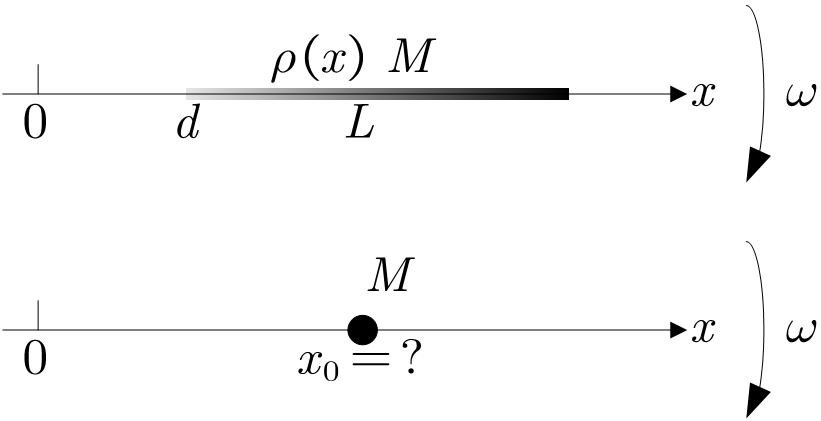
\includegraphics[height=3cm]{4.1.png}
\end{figure}

可以假设细长杆的一个微元可视为质点，则向心力微元和整体向心力：
\begin{align*}
&dF=\rho \left( x \right) dx\cdot \omega ^2\cdot x\quad \left[ \mathrm{N} \right] \\
&F=\int_d^{d+L}{dF}=\int_d^{d+L}{\rho \left( x \right) dx\cdot \omega ^2\cdot x}=\omega ^2\int_d^{d+L}{x\rho \left( x \right) \cdot dx}\quad \left[ \mathrm{N} \right]
\end{align*}
若将其视为质点，则向心力等价为质量$M$的质点小球在$x_0$处以角速度$\omega $匀速转动，有：
\[
\omega ^2\int_d^{d+L}{x\rho \left( x \right) \cdot dx}=M\cdot \omega ^2\cdot x_0\quad \left[ \mathrm{N} \right]
\]
于是可得：
\[
x_0=\frac{\int_d^{d+L}{x\rho \left( x \right) \cdot dx}}{M}=\int_d^{d+L}{x\frac{\rho \left( x \right)}{M}\cdot dx}\quad \left[ \mathrm{m} \right]
\]
对比一维变量的数学期望定义式：
\[
EX=\int_{-\infty}^{+\infty}{xf\left( x \right) \cdot dx}
\]
{\bf 数学期望的物理意义为绕原点匀速转动时的质心位置，有量纲$\left[ \mathrm{m} \right] $}。

简单来讲就是细长杆的质心，之所以要特别强调转动，是为了下面的二维考虑，其次，在考察方差的物理意义时，还会联系转动惯量和平行轴定理。

考虑二维平面，如下图，面密度$\rho \left( x,y \right) $的平面$D$，绕{\it y}轴匀速转动$\omega $ ，在{\it x}轴方向的向心力$F$等效到质点小球$M$产生的向心力。
\begin{figure}[h]
\centering
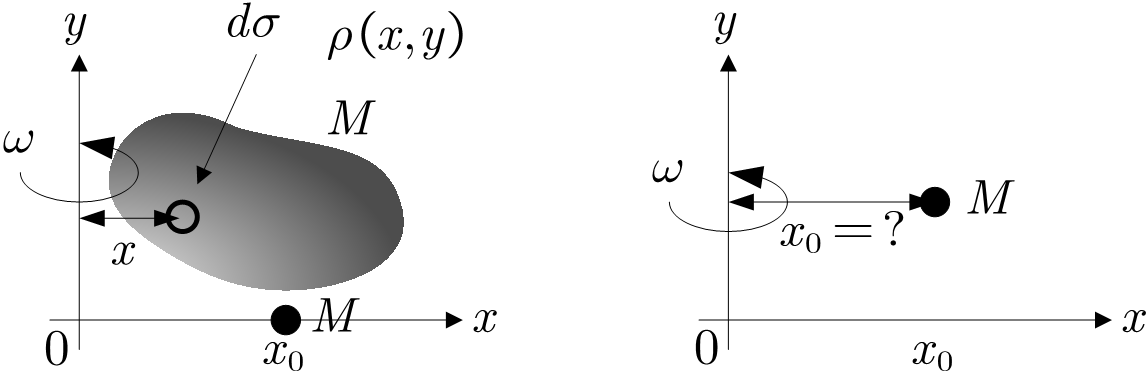
\includegraphics[height=3cm]{4.2.png}
\end{figure}
\begin{align*}
F&=\iint\limits_D{dF}=\iint\limits_D{\rho \left( x,y \right) d\sigma \cdot \omega ^2\cdot x} \\
&=\omega ^2\iint\limits_D{x\rho \left( x,y \right) \cdot d\sigma}=M\cdot \omega ^2\cdot x_0 \quad \left[ \mathrm{N} \right]
\end{align*}
对比二维变量的数学期望定义式：
\[
EX=\iint\limits_{\mathbb{R} \times \mathbb{R}}{xf\left( x,y \right) \cdot d\sigma}
\]
{\bf 二维变量$\left( X,Y \right) $的数学期望$EX$的物理意义为平面绕{\it y}轴匀速转动时在{\it x}方向的质心位置，有量纲$\left[ \mathrm{m} \right] $。}
$EY$的物理意义同样可得，略。

\begin{tcolorbox}
对于函数的数学期望，由于函数无固定形态，所以量纲也无具体表达。
\end{tcolorbox}

%============================================================
\subsection{数学期望的性质}

{\bf 性质1}：常数的数学期望为其本身，即$E\left( c \right) =c$。

{\bf 性质2}：$X\geqslant a\Rightarrow EX\geqslant a,X\leqslant a\Rightarrow EX\leqslant a$

{\bf 性质3}：$E\left( kX \right) =k\cdot E\left( X \right) $

{\bf 性质4}：$E\left( kX+c \right) =k\cdot E\left( X \right) +c$，由性质1+3可证。

{\bf 性质5}：设$\left( X,Y \right) $为二维随机变量，则$E\left( X\pm Y \right) =E\left( X \right) \pm E\left( Y \right) $

{\bf 性质6}：设$\left( X,Y \right) $为二维随机变量，若$X,Y$相互独立$\Rightarrow E\left( XY \right) =E\left( X \right) \cdot E\left( Y \right) $

{\bf 性质7}：设$\left( X,Y \right) $为二维随机变量，则$\left[ E\left( XY \right) \right] ^2\leqslant E\left( X^2 \right) \cdot E\left( Y^2 \right) $

~

性质1表示了常数$c$的分布，其实就是质点小球，自然质心位置为$c$。
\begin{figure}[h]
    \begin{minipage}{0.48\linewidth}
    \centerline{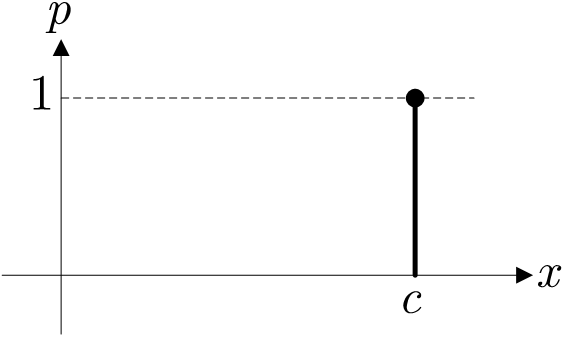
\includegraphics[width=4.5cm]{4.3.png}}
    \end{minipage}
\hfill
    \begin{minipage}{0.48\linewidth}
    \[
    X\sim \left( \begin{array}{l} c\\ 1\\ \end{array} \right)
    \]
    \end{minipage}
\end{figure}

性质2表示了质心的范围，物理意义也很明显，质心位置肯定不会落到物体之外。
\begin{figure}[h]
\centering
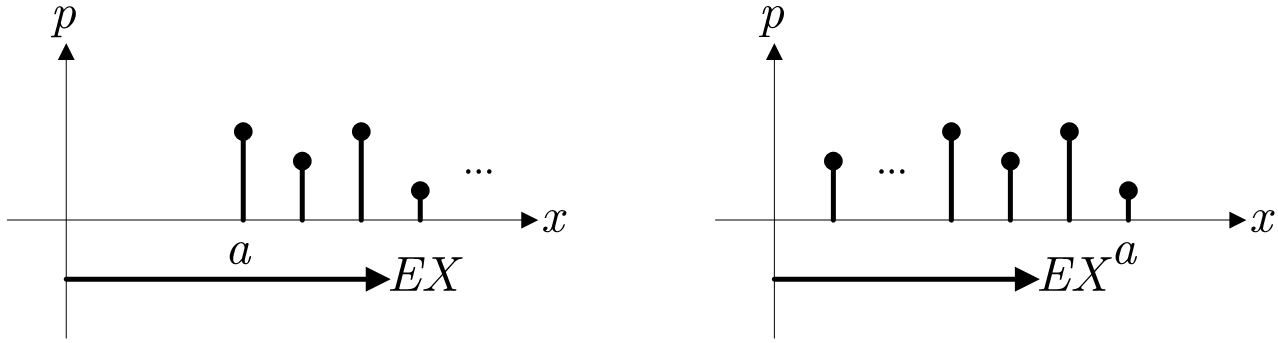
\includegraphics[height=2.5cm]{4.4.png}
\end{figure}

性质3表达当{\it x}轴拉伸时，质心也有同样的拉伸，压缩亦然。
\begin{figure}[h]
\centering
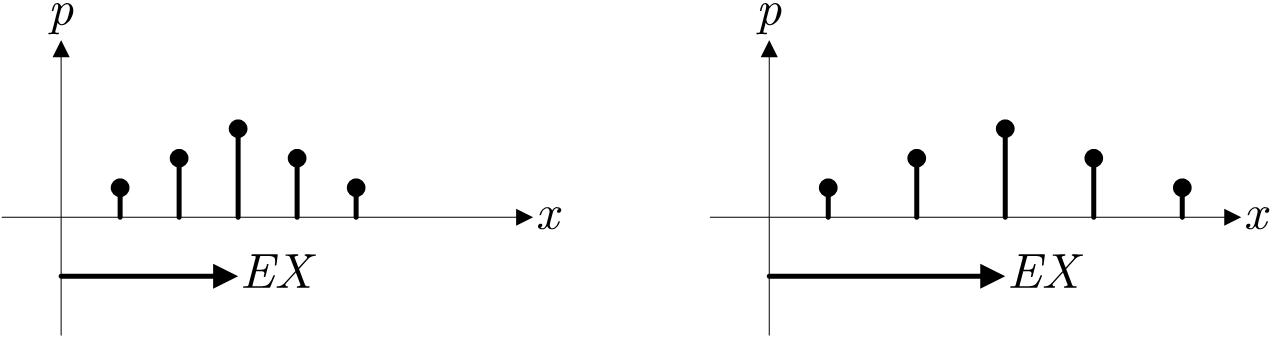
\includegraphics[height=2.5cm]{4.5.png}
\end{figure}

\begin{tcolorbox}
这三个性质可结合物理意义理解。
\end{tcolorbox}

性质5用定义即可证明：
\begin{align*}
E\left( X\pm Y \right) &=\sum_{i=1}^{+\infty}{\sum_{j=1}^{+\infty}{\left( x_i\pm y_j \right) \cdot p_{ij}}}=\sum_{i=1}^{+\infty}{\sum_{j=1}^{+\infty}{\left( x_ip_{ij}\pm y_jp_{ij} \right)}} \\
&=\sum_{i=1}^{+\infty}{\sum_{j=1}^{+\infty}{x_ip_{ij}}}\pm \sum_{i=1}^{+\infty}{\sum_{j=1}^{+\infty}{y_jp_{ij}}} \\
&=E\left( X \right) \pm E\left( Y \right)
\end{align*}

性质6，独立则有$p_{ij}=p_{i\cdot}\cdot p_{\cdot j}$，于是：
\begin{align*}
E\left( XY \right) &=\sum_{i=1}^{+\infty}{\sum_{j=1}^{+\infty}{\left( x_iy_j \right) \cdot p_{ij}}}=\sum_{i=1}^{+\infty}{\sum_{j=1}^{+\infty}{\left( x_iy_j \right) \cdot p_{i\cdot}\cdot p_{\cdot j}}} \\
&=\sum_{i=1}^{+\infty}{\left( x_ip_{i\cdot}\cdot \sum_{j=1}^{+\infty}{y_jp_{\cdot j}} \right)}=\sum_{i=1}^{+\infty}{\left[ x_ip_{i\cdot}\cdot E\left( Y \right) \right]} \\
&=E\left( X \right) \cdot E\left( Y \right)
\end{align*}

\begin{tcolorbox}
数学期望的性质常用于随机变量组合成新变量的数学期望的计算。
由于数学期望是线性运算，所以有
\[
E\left( aX+bY+c \right) =aEX+bEY+c
\]
但对于非线性组合，会有一些前置条件或者为不等式。
\end{tcolorbox}

\begin{tcolorbox}
$\left( EX \right) ^2$不大于$E\left( X^2 \right) $，证明关系留到介绍方差后再给出。
\end{tcolorbox}

%============================================================
\subsection{数学期望的范围}

数学期望的范围是变量的范围，这点从数学期望的物理意义也很好理解，特别是当变量的分布为常数分布时，取到最大值。
此时，随机事件变成确定性事件。对应地，函数的数学期望的范围是函数的值域。
\begin{figure}[h]
    \begin{minipage}{0.48\linewidth}
    \centerline{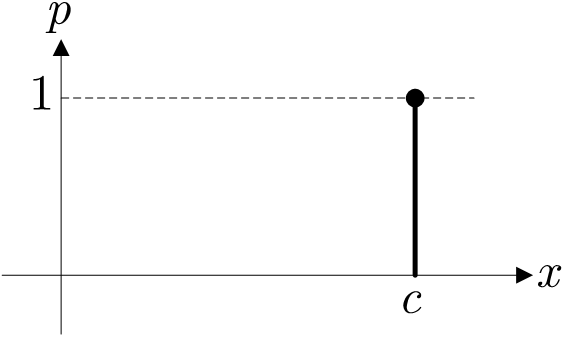
\includegraphics[width=4.5cm]{4.3.png}}
    \end{minipage}
\hfill
    \begin{minipage}{0.48\linewidth}
    \[
    X\sim \left( \begin{array}{l} c\\ 1\\ \end{array} \right)
    \]
    \end{minipage}
\end{figure}

%============================================================
\subsection{中位数的概念}

\begin{definition}[中位数]
若随机变量$X$有分布函数$F\left( x \right) $，若$m$满足
\[
F\left( m \right) =\frac{1}{2}
\]
则称$m$为{\bf 随机变量$X$的中位数}。
\end{definition}

数学期望和中位数都反映了随机变量的一个均值情况。中位数表示了该点前后的概率是一样的，优点是受特大值、特小值影响小，而且必然存在，缺点是处理不方便（如两个随机变量加减乘除后的中位数），而且不唯一，特别在离散型随机变量，由于取值的离散型，中位数大多不会精确的存在。

%============================================================
\subsection{例}

\begin{example}
若盒子中有2个红球1个白球，先分别采取不放回抽取和放回抽取两种策略，记$X$为首次抽中红球时的取球的次数，分别计算$EX$。
\end{example}

解：

1. 不放回抽取时，$X$只能为$1,2$，且易得$P\left\{ X=1 \right\} =\frac{2}{3},P\left\{ X=2 \right\} =\frac{1}{3}\cdot \frac{2}{2}=\frac{1}{3}$，于是：
\[
EX=1\cdot \frac{2}{3}+2\cdot \frac{1}{3}=\frac{4}{3}
\]

2. 放回抽取时，$X=1,2,\cdots $，且有$P\left\{ X=i \right\} =\left( \frac{1}{3} \right) ^{i-1}\cdot \frac{2}{3}$，于是$EX=\frac{2}{3}\cdot \sum_{i=1}^{+\infty}{i\cdot \left( \frac{1}{3} \right) ^{i-1}}$，对于该无穷级数，等号两边都乘以$1/3$：
\begin{align*}
&\because \frac{1}{3}EX=\frac{2}{3}\cdot \sum_{i=1}^{+\infty}{i\cdot \left( \frac{1}{3} \right) ^i} \\
&\begin{aligned}
	\therefore \frac{2}{3}EX&=EX-\frac{1}{3}EX=\frac{2}{3}\cdot \left[ \sum_{i=1}^{+\infty}{i\cdot \left( \frac{1}{3} \right) ^{i-1}}-\sum_{i=1}^{+\infty}{i\cdot \left( \frac{1}{3} \right) ^i} \right]\\
	&=\frac{2}{3}\cdot \sum_{i=1}^{+\infty}{\left( \frac{1}{3} \right) ^{i-1}}=\frac{2}{3}\cdot \frac{1}{1-\frac{1}{3}}=1\\
\end{aligned} \\
&\therefore EX=\frac{3}{2}
\end{align*}

~

\begin{example}
若变量$X$的密度函数$f\left( x \right) =2x,x\in \left( 0,1 \right) $，求$X$和$X^2$的数学期望。
\end{example}

解：
\begin{align*}
&E\left( X \right) =\int_{-\infty}^{+\infty}{xf\left( x \right) \cdot dx}=\int_0^1{x\cdot 2x\cdot dx}=\left. \frac{2}{3}x^3 \right|_{0}^{1}=\frac{2}{3} \\
&E\left( X^2 \right) =\int_{-\infty}^{+\infty}{x^2f\left( x \right) \cdot dx}=\int_0^1{x^2\cdot 2x\cdot dx}=\left. \frac{1}{2}x^4 \right|_{0}^{1}=\frac{1}{2}
\end{align*}

~

\begin{example}
设离散随机变量$X$和连续随机变量$Y$如下
\begin{align*}
&X~\left( \begin{matrix}
    0&		10\\
    \frac{3}{5}&		\frac{2}{5}\\
\end{matrix} \right) \\
&f\left( y \right) =\frac{1}{2}e^{-\left| y \right|}
\end{align*}
且$X,Y$相互独立，求$E\left( XY^2-2X^2Y+1 \right) $。
\end{example}

解：

由于且$X,Y$相互独立，所以$X,Y^2$相互独立、$X^2,Y$相互独立，于是：
\begin{align*}
E\left( XY^2-2X^2Y+1 \right) &=E\left( XY^2 \right) -2E\left( X^2Y \right) +E\left( 1 \right) \\
&=E\left( X \right) \cdot E\left( Y^2 \right) -2E\left( X^2 \right) \cdot E\left( Y \right) +1
\end{align*}
先分别计算$E\left( X \right) $、$E\left( X^2 \right) $、$E\left( Y \right) $和$E\left( Y^2 \right) $，然后计算结果：
\begin{align*}
&\because \begin{cases}
	E\left( X \right) =0\cdot \frac{3}{5}+10\cdot \frac{2}{5}=4\\
	E\left( X^2 \right) =0^2\cdot \frac{3}{5}+10^2\cdot \frac{2}{5}=40\\
	E\left( Y \right) =\int_{-\infty}^{+\infty}{y\frac{1}{2}e^{-\left| y \right|}\cdot dy}=0\\
	E\left( Y^2 \right) =\int_{-\infty}^{+\infty}{y^2\frac{1}{2}e^{-\left| y \right|}\cdot dy}=\int_0^{+\infty}{y^2e^{-y}\cdot dy}=2\\
\end{cases} \\
&\therefore E\left( X \right) \cdot E\left( Y^2 \right) -2E\left( X^2 \right) \cdot E\left( Y \right) +1=4\cdot 2-2\cdot 40\cdot 0+1=9
\end{align*}






\newpage
\section{方差}

本节介绍随机变量的第二个重要数字特征——方差。

本节要点：
\begin{itemize}
    \item 掌握方差的概念；
    \item 理解方差的统计意义和物理意义。
\end{itemize}

%============================================================
\subsection{一维随机变量方差的概念}

\begin{definition}[一维随机变量的方差]
设一维随机变量$X$，若函数$\left( X-EX \right) ^2$的数学期望存在，则称该数学期望为{\bf 一维随机变量$X$的方差}，记作$D\left( X \right) $或$DX$，即：
\begin{align*}
&DX:=E\left[ \left( X-EX \right) ^2 \right] =\sum_{i=1}^{+\infty}{\left( x_i-EX \right) ^2\cdot p_i} \\
&DX:=E\left[ \left( X-EX \right) ^2 \right] =\int_{-\infty}^{+\infty}{\left( x-EX \right) ^2f\left( x \right) \cdot dx}
\end{align*}
同时称$\sqrt{DX}$为{\bf $X$的平方差}。
\end{definition}

\begin{tcolorbox}
方差的英文为Variance，“教材\cite{book2}”中使用$\mathrm{Var}\left( X \right) $作为记号。
\end{tcolorbox}

方差的求解较为繁琐，由于$\left( X-EX \right) ^2=X^2-2\cdot X\cdot EX+\left( EX \right) ^2$，且$EX$是常数，利用数学期望的性质可得便捷公式：
\begin{align*}
DX&=E\left[ X^2-2\cdot X\cdot EX+\left( EX \right) ^2 \right] \\
&=E\left( X^2 \right) -2\cdot EX\cdot EX+\left( EX \right) ^2 \\
&=E\left( X^2 \right) -\left( EX \right) ^2
\end{align*}

从便捷公式可以得到$\left[ E\left( X \right) \right] ^2$和$E\left( X^2 \right) $的关系：
\[
E\left( X^2 \right) =DX+\left( EX \right) ^2
\]
由于$DX\geqslant 0$，所以$E\left( X^2 \right) \geqslant \left( EX \right) ^2$。

\begin{tcolorbox}
由于数学期望的线性性，便捷公式的推导没有任何前置条件，所以被广泛使用，定义式则更多用来理解概念。
\end{tcolorbox}

%============================================================
\subsection{二维随机变量函数的方差}

\begin{tcolorbox}
在二维变量中，我们更多考虑两个变量组合函数的方差。
\end{tcolorbox}

\begin{definition}[二维随机变量函数的方差]
设二维随机变量$\left( X,Y \right) $，若有$Z=z\left( X,Y \right) $且根据定义的对应级数或积分绝对收敛，具体定义式略，则称相应的级数或积分为{\bf $Z=z\left( X,Y \right) $的方差}，可采用便利公式计算，如下：
\[
DZ=E\left[ z\left( X,Y \right) ^2 \right] -E\left[ z\left( X,Y \right) \right] ^2
\]
\end{definition}

%============================================================
\subsection{方差的数学由来和统计意义}

方差定义中，$X-EX$是根本，表示了随机变量$X$和它的均值$EX$的偏离程度。
由于$E\left( X-EX \right) =E\left( X \right) -EX=0$，总是为0，所以我们取绝对值$\left| X-EX \right|$，又由于绝对值函数在0点不可导，所以我们替换成平方$\left( X-EX \right) ^2$定义方差。

方差描述了随机变量$X$偏离其数学期望的程度，$DX$越小，说明离散程度越小。

%============================================================
\subsection{方差的物理意义}

考虑一维物体的转动。
长度为$L$的细长杆质量$M$且分布不均匀，有线密度$\rho \left( x \right) ,x\in \left[ d,d+L \right] $，一端距原点$d$，绕原点转动，如下图。
\begin{figure}[h]
\centering
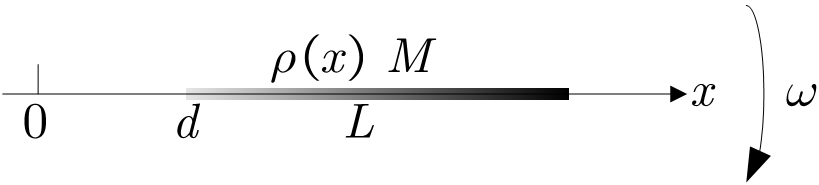
\includegraphics[height=1.5cm]{4.6.png}
\end{figure}

其转动惯量$I$有：
\[
I=\int{x^2\cdot dM}=\int_d^{d+L}{x^2\cdot \rho \left( x \right) \cdot dx} \quad \left[ \mathrm{kg}\cdot \mathrm{m}^2 \right]
\]
若将转轴移到质心$x_0$ ，根据平行轴定理，新的转动惯量$I_{x_0}$有：
\begin{align*}
&\because I=I_{x_0}+{Mx_0}^2 \\
&\therefore \int_d^{d+L}{x^2\cdot \rho \left( x \right) \cdot dx}=I_{x_0}+{Mx_0}^2 \\
&\therefore \int_d^{d+L}{x^2\cdot \frac{\rho \left( x \right)}{M}\cdot dx}=\frac{I_{x_0}}{M}+{x_0}^2
\end{align*}
对比方差的便捷计算公式：
\[
E\left( X^2 \right) =\int_{-\infty}^{+\infty}{x^2f\left( x \right) \cdot dx}=DX+\left( EX \right) ^2
\]
显然，{\bf 方差的物理意义可以理解为物体以质心为原点时的单位质量的转动惯量，有量纲$\left[ \mathrm{m}^2 \right] $}。
跟物理的转动惯量不一样，没有质量这个因子，所以描述的是一种和具体质量无关的惰性，这种惰性和分布有关，$DX$越大，说明分布越靠外，转动惯量也越大。

考虑二维平面，面密度$\rho \left( x,y \right) $的平面$D$，绕{\it y}轴匀速转动，如下左图：
\begin{figure}[h]
\centering
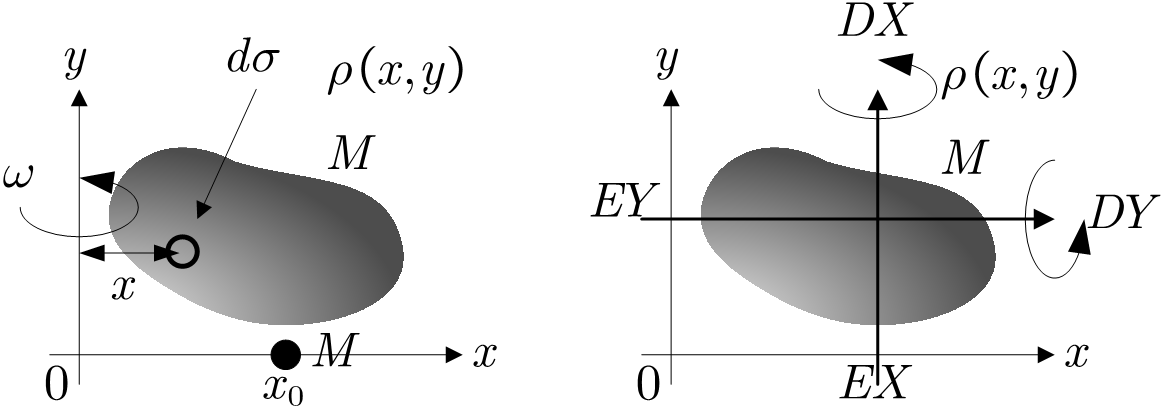
\includegraphics[height=3cm]{4.7.png}
\end{figure}

其转动惯量$I$有：
\[
I=\iint\limits_D{x^2\cdot \rho \left( x,y \right) \cdot d\sigma} \quad \left[ \mathrm{kg}\cdot \mathrm{m}^2 \right]
\]
对比二维变量的方差：
\[
DX=\iint\limits_{\mathbb{R} \times \mathbb{R}}{\left( x-EX \right) ^2f\left( x,y \right) \cdot d\sigma}
\]
{\bf 二维变量$\left( X,Y \right) $的方差$DX$的物理意义为在绕轴$x=x_0$竖直转动时，单位质量的转动惯量，有量纲$\left[ \mathrm{m}^2 \right] $。}
同样方差$DY$的物理意义为在绕轴$y=y_0$水平转动时，单位质量的转动惯量，也有量纲$\left[ \mathrm{m}^2 \right] $，如上右图。

%============================================================
\subsection{方差的性质}

{\bf 性质1}：常数的方差为0，即$D\left( c \right) =0$。

{\bf 推论}：$D\left( X \right) \geqslant 0$，当且仅当$P\left\{ X=EX \right\} =1$时（即常数分布），等号成立。

{\bf 性质2}：$D\left( kX \right) =k^2\cdot DX$

{\bf 性质3}：$D\left( kX+c \right) =k^2\cdot DX$，由性质1，2可得。

{\bf 性质4}：设$\left( X,Y \right) $为二维随机变量，

若$X,Y$相互独立$\Rightarrow D\left( X\pm Y \right) =DX+DY$

进一步地，若$X,Y$相互独立$\Rightarrow D\left( aX\pm bY \right) =a^2\cdot DX+b^2\cdot DY$

~

性质1，对于常数分布，质心就是$c$，显然绕质心的转动惯量为0。

性质2，若$X\rightarrow kX$，相当于直线被拉长$k$倍，自然转动惯量扩大了$k^2$倍。

\begin{figure}[h]
\centering
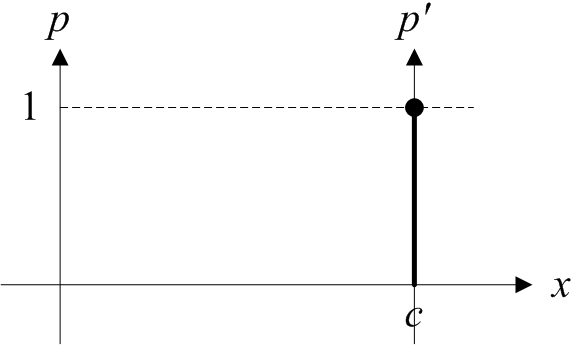
\includegraphics[height=2.5cm]{4.8.png}
\end{figure}

\begin{tcolorbox}
上述性质可结合物理意义理解。
\end{tcolorbox}

性质4，证明如下：
\begin{align*}
&\because DX=E\left( X^2 \right) -\left( EX \right) ^2 \\
&\begin{aligned}
	\therefore D\left( X\pm Y \right) &=E\left[ \left( X\pm Y \right) ^2 \right] -E\left[ \left( X\pm Y \right) \right] \cdot E\left[ \left( X\pm Y \right) \right]\\
	&=E\left[ X^2\pm 2XY+Y^2 \right] -\left[ EX\pm EY \right] ^2\\
	&=\left[ E\left( X^2 \right) \pm 2E\left( XY \right) +E\left( Y^2 \right) \right] -\\
	&\left[ \left( EX \right) ^2\pm 2\left( EX \right) \left( EY \right) +\left( EY \right) ^2 \right]\\
\end{aligned} \\
&\because E\left( XY \right) =\left( EX \right) \left( EY \right) \\
&\begin{aligned}
	\therefore D\left( X\pm Y \right) &=\left[ E\left( X^2 \right) -\left( EX \right) ^2 \right] +\left[ E\left( Y^2 \right) -\left( EY \right) ^2 \right]\\
	&=DX+DY\\
\end{aligned}
\end{align*}

%============================================================
\subsection{方差的取值范围}

变量的方差的取值范围根据不同的分布有不同的范围。如常数分布，中心点转动惯量必然为0。
又如$P\left\{ X=\pm \infty \right\} =0.5$，显然转动惯量$+\infty $ 。

\begin{figure}[h]
\centering
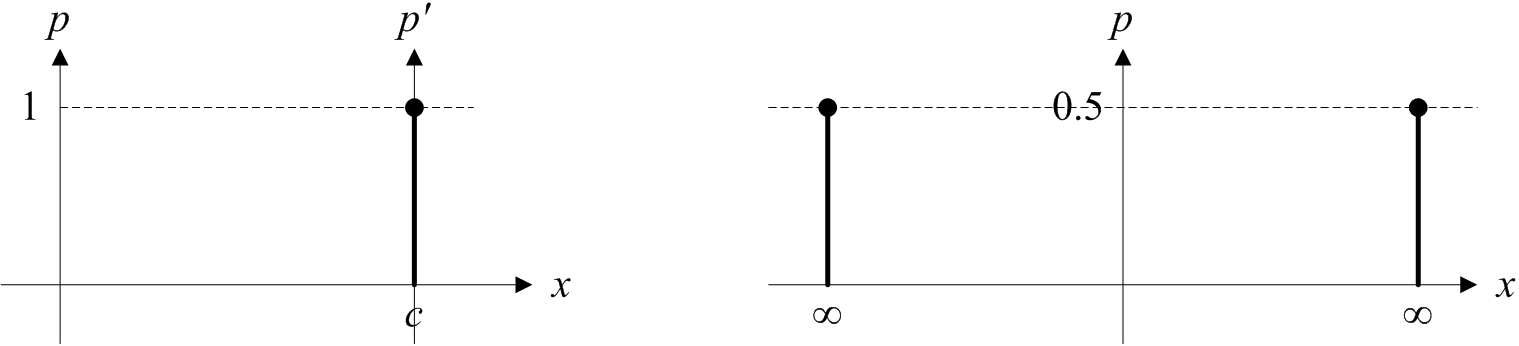
\includegraphics[height=2.5cm]{4.9.png}
\end{figure}

%============================================================
\subsection{随机变量的标准化}

\begin{definition}[随机变量的标准化]
设随机变量$X$有数学期望$EX$和方差$DX>0$，若将$X$进行运算$\frac{X-EX}{\sqrt{DX}}$，获得的随机变量称为{\bf $X$的标准化随机变量}，记作$X^*$，即：
\[
X^*=\frac{X-EX}{\sqrt{DX}}
\]
且有：
\begin{align*}
&E\left( X^* \right) =E\left( \frac{X-EX}{\sqrt{DX}} \right) =\frac{1}{\sqrt{DX}}\cdot E\left( X-EX \right) =0 \\
&D\left( X^* \right) =D\left( \frac{X-EX}{\sqrt{DX}} \right) =\frac{1}{DX}\cdot D\left( X-EX \right) =1
\end{align*}
\end{definition}

~

考察标准化过程：
\begin{itemize}
    \item $X-EX$:表示将坐标原点拉到期望$EX$的位置，即原点对称；
    \item $\frac{1}{\sqrt{DX}}$：拉伸或收缩{\it x}轴，使得分布不过于稀疏或稠密。
\end{itemize}
排除这两个“干扰”后，很多初看起来不同的分布，实际是一类分布，有利于后续的进一步分析。
如不同的正态分布，标准化之后就是标准正态分布。






\newpage
\section{常见分布的数学期望和方差}

本节讨论几个常见分布的数学期望和方差。

%============================================================
\subsection{0-1分布}

0-1分布$B\left( 1,p \right) $，$P\left\{ X=x \right\} =p^x\left( 1-p \right) ^{1-x},\quad x=0,1$：
\begin{align*}
&EX=p \\
&DX=p-p^2
\end{align*}

%============================================================
\subsection{二项分布}

二项分布$B\left( n,p \right) $，$P\left\{ X=x \right\} =C_{n}^{x}p^x\left( 1-p \right) ^{n-x},\quad x=0,1,\cdots ,n$：
\begin{align*}
&EX=np \\
&DX=np\left( 1-p \right)
\end{align*}

%============================================================
\subsection{泊松分布}

泊松分布$P\left( \lambda \right) $，$P\left\{ X=x \right\} =\frac{\lambda ^x}{x!}e^{-\lambda},\quad x=0,1,2,\cdots $：
\begin{align*}
&EX=\lambda \\
&DX=\lambda
\end{align*}
配合例图，$\lambda =np$越大，质心越远，转动惯量也越大。
\begin{figure}[h]
\centering
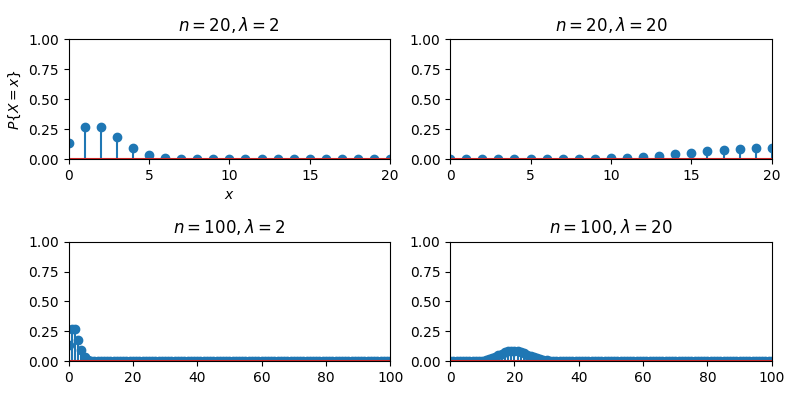
\includegraphics[height=5cm]{2.5.png}
\end{figure}

%============================================================
\subsection{几何分布}

几何分布$G\left( p \right) $，$P\left\{ X=x \right\} =p\left( 1-p \right) ^{x-1},\quad x=1,2,\cdots $：
\begin{align*}
&EX=\frac{1}{p} \\
&DX=\frac{1-p}{p^2}
\end{align*}
配合例图，$p$越大，质心越近，转动惯量也越小。
\begin{figure}[h]
\centering
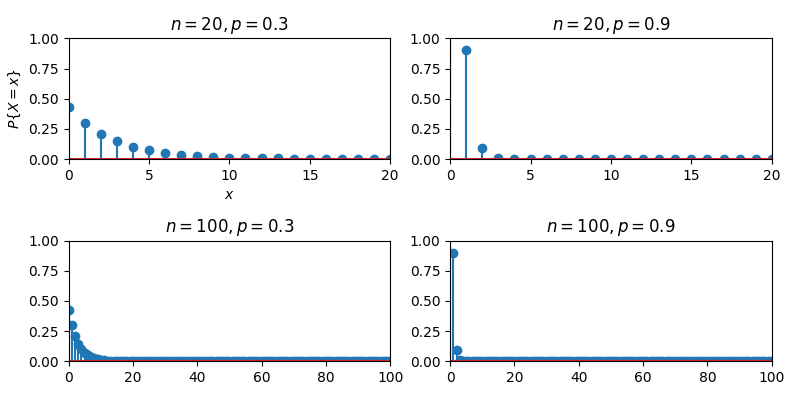
\includegraphics[height=5cm]{2.6.png}
\end{figure}

%============================================================
\subsection{超几何分布}

超几何分布$H\left( M,N,n \right) $，$P\left\{ X=x \right\} =\frac{C_{N-M}^{n-x}C_{M}^{x}}{C_{N}^{n}}$：
\begin{align*}
&EX=\frac{nM}{N} \\
&DX=\frac{nM\left( N-n \right) \left( N-M \right)}{N^2\left( N-1 \right)}
\end{align*}

%============================================================
\subsection{均匀分布}
均匀分布$U\left[ a,b \right] $，$f\left( x \right) =\begin{cases}
	\frac{1}{b-a},&		x\in \left[ a,b \right]\\
	0,&		x\notin \left[ a,b \right]\\
\end{cases}$：
\begin{align*}
&EX=\frac{a+b}{2} \\
&DX=\frac{1}{12}\left( b-a \right) ^2
\end{align*}

%============================================================
\subsection{指数分布}

指数分布$E\left( \lambda \right) $，$f\left( x \right) =\begin{cases}
	0,&		x<0\\
	\lambda e^{-\lambda x},&		x\geqslant 0\\
\end{cases}$：
\begin{align*}
&EX=\frac{1}{\lambda} \\
&DX=\frac{1}{\lambda ^2}
\end{align*}
配合例图，$\lambda $越大，质心越近，转动惯量也越小。
\begin{figure}[h]
\centering
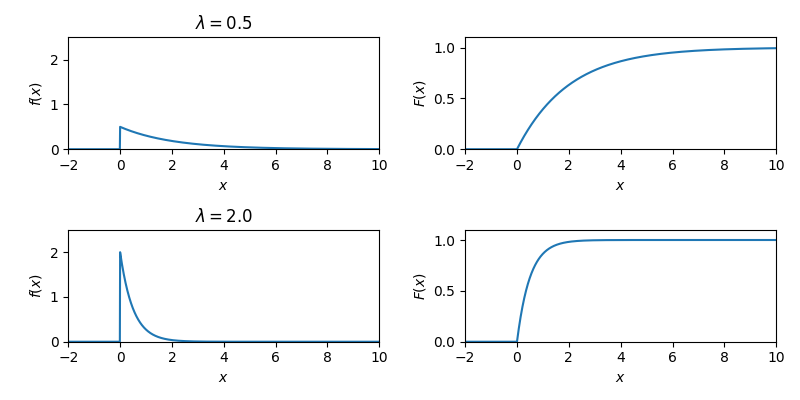
\includegraphics[height=5cm]{2.9.png}
\end{figure}

考察标准化指数分布：
\begin{align*}
&\because \begin{cases}
	X^*=\frac{X-EX}{\sqrt{DX}}\\
	X=\sqrt{DX}\cdot X^*+EX\\
\end{cases} \\
&\therefore \begin{cases}
	g^{-1}\left( X^* \right) =\sqrt{DX}\cdot X^*+EX\\
	\left| \frac{dg^{-1}\left( Y \right)}{dY} \right|=\sqrt{DX}\\
\end{cases} \\
&\begin{aligned}
	\therefore f\left( x^* \right) &=f_X\left[ g^{-1}\left( X^* \right) \right] \cdot \left| \frac{dg^{-1}\left( X^* \right)}{dX^*} \right|\\
	&=\lambda e^{-\lambda \left( \sqrt{DX}\cdot x^*+EX \right)}\cdot \sqrt{DX}=\lambda e^{-\lambda \left( \frac{1}{\lambda}\cdot x^*+\frac{1}{\lambda} \right)}\cdot \frac{1}{\lambda}\\
	&=e^{-\left( x^*+1 \right)}\\
\end{aligned}
\end{align*}
其中，$x^*\geqslant -1$，所以标准化的分布函数：
\[
F\left( x^* \right) =\int_{-1}^{+\infty}{f\left( t \right) \cdot dt}=\int_{-1}^{x^*}{e^{-\left( t+1 \right)}\cdot dt}=1-e^{-\left( x^*+1 \right)}
\]
\begin{figure}[ht]
\centering
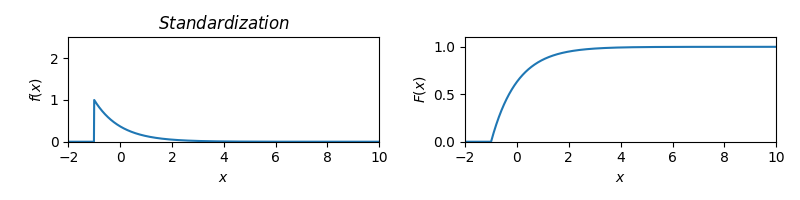
\includegraphics[height=2.5cm]{4.10.png}
\end{figure}

%============================================================
\subsection{正态分布}

正态分布$N\left( \mu ,\sigma ^2 \right) $，$f\left( x \right) =\frac{1}{\sqrt{2\pi}\sigma}e^{-\frac{\left( x-\mu \right) ^2}{2\sigma ^2}} \quad \mu \in \mathbb{R} ,\sigma >0$：
\begin{align*}
&EX=\mu \\
&DX=\sigma ^2
\end{align*}
标准正态分布$N\left( 0,1 \right) $，$\varphi \left( x \right) =\frac{1}{\sqrt{2\pi}}e^{-\frac{x^2}{2}}$：
\begin{align*}
&EX=0 \\
&DX=1
\end{align*}
配合例图，$\mu $决定了质心的位置，$\sigma ^2$决定了转动惯量。

\begin{figure}[h]
\centering
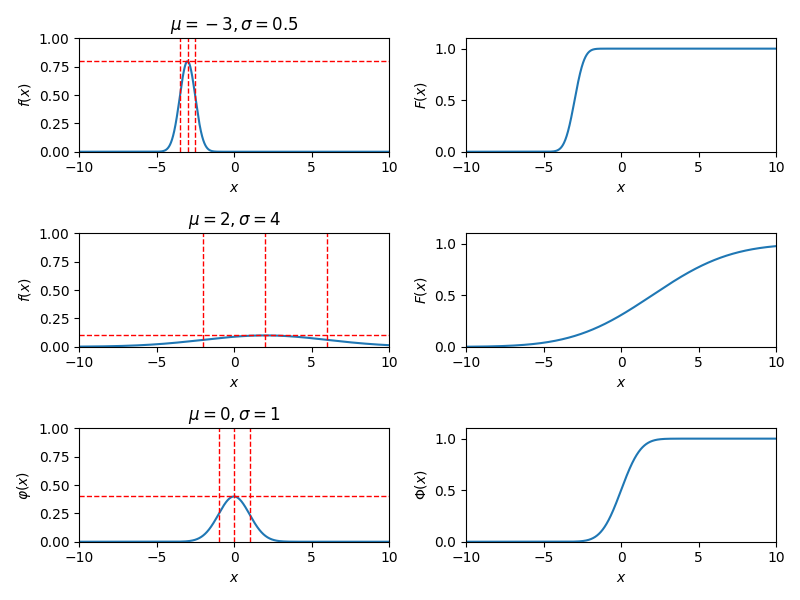
\includegraphics[height=7.5cm]{2.10.png}
\end{figure}






\newpage
\section{协方差和相关系数}

前面介绍的数学期望和方差，无论是否为二维变量，最终考察的总是一维变量的数字特征。
本节介绍描述两个变量之间关系的数字特征——协方差和相关系数。

本节要点：
\begin{itemize}
    \item 掌握协方差的概念；
    \item 掌握相关系数的概念；
    \item 深刻理解相关系数的由来及几何意义。
\end{itemize}

%============================================================
\subsection{协方差的概念}

\begin{definition}[协方差]
设二维随机变量$\left( X,Y \right) $，若存在数学期望
\[
E\left[ \left( X-EX \right) \left( Y-EY \right) \right]
\]
则称之为{\bf $X$和$Y$的协方差}，记作$\mathrm{Cov}\left( X,Y \right) $，即：
\begin{align*}
\mathrm{Cov}\left( X,Y \right) :&=\sum_i{\sum_j{\left( x_i-EX \right) \cdot \left( y_j-EY \right) \cdot p_{ij}}} \\
\mathrm{Cov}\left( X,Y \right) :&=\iint\limits_{\mathbb{R} \times \mathbb{R}}{\left( x-EX \right) \cdot \left( y-EY \right) \cdot f\left( x,y \right) \cdot d\sigma}, \quad d\sigma =dxdy
\end{align*}
\end{definition}

由数学期望和方差的性质可得便捷计算公式：
\begin{align*}
\mathrm{Cov}\left( X,Y \right) &=E\left[ \left( X-EX \right) \left( Y-EY \right) \right] \\
&=E\left[ XY-X\cdot EY-Y\cdot EX+EX\cdot EY \right] \\
&=E\left( XY \right) -EY\cdot E\left( X \right) -EX\cdot E\left( Y \right) +E\left( EX\cdot EY \right) \\
&=E\left( XY \right) -EX\cdot EY
\end{align*}
特别地，当$X$和$Y$相互独立时$E\left( XY \right) =E\left( X \right) \cdot E\left( Y \right) $，有：
\[
\mathrm{Cov}\left( X,Y \right) =E\left( X \right) \cdot E\left( Y \right) -EX\cdot EY=0
\]

\begin{tcolorbox}
$\mathrm{Cov}$是“Covariance”的缩写。同样定义式更多的是为了理解概念，实际中通常使用便捷公式。
\end{tcolorbox}

%============================================================
\subsection{协方差的性质}

{\bf 性质1}：$\mathrm{Cov}\left( X,X \right) =DX$

{\bf 性质2}：$\mathrm{Cov}\left( X,c \right) =0$

{\bf 性质3}：设$\left( X,Y \right) $为二维随机变量，

$D\left( X\pm Y \right) =DX+DY\pm 2\mathrm{Cov}\left( X,Y \right) $

{\bf 性质4}：设$\left( X,Y \right) $为二维随机变量，$\mathrm{Cov}\left( X,Y \right) =\mathrm{Cov}\left( Y,X \right) $

{\bf 性质5}：设$\left( X,Y \right) $为二维随机变量，$\left[ \mathrm{Cov}\left( X,Y \right) \right] ^2\leqslant DX\cdot DY$

{\bf 性质6}：设$\left( X,Y \right) $为二维随机变量，$\mathrm{Cov}\left( aX,bY \right) =ab\mathrm{Cov}\left( X,Y \right) $

{\bf 性质7}：设$\left( X_1,X_2,Y \right) $为三维随机变量，

$\mathrm{Cov}\left( X_1\pm X_2,Y \right) =\mathrm{Cov}\left( X_1,Y \right) \pm \mathrm{Cov}\left( X_2,Y \right) $

~

性质1，用各自的便捷公式即可证明：
\[
\mathrm{Cov}\left( X,X \right) =E\left( X^2 \right) -\left( EX \right) ^2=DX
\]

性质3，用各自的便捷公式也可证明：
\begin{align*}
D\left( X\pm Y \right) &=\left[ E\left( X^2 \right) \pm 2E\left( XY \right) +E\left( Y^2 \right) \right] - \\
&\left[ \left( EX \right) ^2\pm 2\left( EX \right) \left( EY \right) +\left( EY \right) ^2 \right] \\
&=DX+DY\pm 2\left[ E\left( XY \right) +\left( EX \right) \left( EY \right) \right] \\
&=DX+DY\pm 2\mathrm{Cov}\left( X,Y \right)
\end{align*}

\begin{tcolorbox}
上述两个性质联系了方差和协方差，特别是性质3，可配合方差性质：
\[
\text{若}X,Y\text{相互独立}\Rightarrow D\left( X\pm Y \right) =D\left( X \right) +D\left( Y \right)
\]
进行理解。
\end{tcolorbox}

性质5，是理解相关系数的关键，证明如下：
\begin{align*}
&\because \mathrm{Cov}\left( X,Y \right) =E\left[ \left( X-EX \right) \left( Y-EY \right) \right] \\
&\because \left[ E\left( XY \right) \right] ^2\leqslant E\left( X^2 \right) \cdot E\left( Y^2 \right) \\
&\begin{aligned}
	\therefore \left[ \mathrm{Cov}\left( X,Y \right) \right] ^2&=\left[ E\left[ \left( X-EX \right) \left( Y-EY \right) \right] \right] ^2\\
	&\leqslant E\left[ \left( X-EX \right) ^2 \right] \cdot E\left[ \left( Y-EY \right) ^2 \right] =DX\cdot DY\\
\end{aligned}
\end{align*}

%============================================================
\subsection{协方差的统计意义}
从协方差的定义入手：
\[
\mathrm{Cov}\left( X,Y \right) :=\sum_i{\sum_j{\left( x_i-EX \right) \cdot \left( y_j-EY \right) \cdot p_{ij}}}
\]

\begin{itemize}
    \item $\left( x_i-EX \right) \cdot \left( y_j-EY \right) $：表示样本点对均值构成的矩形面积，且1、3象限取正，2、4象限取负；
    \item $\sum_i{\sum_j{\cdot p_{ij}}}$：表示对这些面积加权和。
\end{itemize}
可见：
\begin{itemize}
    \item 当$\mathrm{Cov}\left( X,Y \right) >0$时，表示1、3象限居多，统计上，对于一个样本，$X$取大值时，可能$Y$也是大值；
    \item 反之，当$\mathrm{Cov}\left( X,Y \right) <0$时，统计上，对于一个样本，$X$取大值时，$Y$反倒可能是小值。
\end{itemize}
协方差就表示了$X$和$Y$在分布上有的这个关系，但协方差没有去除$X,Y$各自的方差，下面的相关系数除去了方差的影响，更能精准地刻画$X$和$Y$在分布上的关系。

%============================================================
\subsection{相关系数和不相关的概念}

\begin{definition}[相关系数]
设二维随机变量$\left( X,Y \right) $，若$DX>0,DY>0$，则称$\frac{\mathrm{Cov}\left( X,Y \right)}{\sqrt{DX}\cdot \sqrt{DY}}$为{\bf 二维随机变量$\left( X,Y \right) $的相关系数}，记作$\rho _{XY}$或$\rho $，即：
\[
\rho _{XY}:=\frac{\mathrm{Cov}\left( X,Y \right)}{\sqrt{DX}\cdot \sqrt{DY}}
\]
\end{definition}

由各自的便捷公式可得相关系数的便捷公式：
\[
\rho _{XY}=\frac{\mathrm{Cov}\left( X,Y \right)}{\sqrt{DX}\cdot \sqrt{DY}}=\frac{E\left( XY \right) -EX\cdot EY}{\sqrt{E\left( X^2 \right) -\left( EX \right) ^2}\cdot \sqrt{E\left( Y^2 \right) -\left( EY \right) ^2}}
\]

\begin{definition}[不相关]
对于二维变量$\left( X,Y \right) $，若$\rho _{XY}=0$，则称它们{\bf 不相关}。
\end{definition}

不相关指的是$X,Y$没有线性关系，不排除有其他关系，如平方关系，三角函数关系等，所以不相关是一个比独立要弱的要求。
$X,Y$不相关并不一定独立，而独立必然不相关。

\begin{theorem}
若$X,Y$独立且$\rho _{XY}$存在，则$X,Y$不相关。
\end{theorem}

简单来说即，独立$\Rightarrow $不相关，还是要注意反命题不成立。

\begin{theorem}
若二维变量$\left( X,Y \right) $存在$\rho _{XY}$，则下列命题等价：
\begin{itemize}
    \item $X,Y$不相关；
    \item $\rho _{XY}=0$
    \item $\mathrm{Cov}\left( X,Y \right) =0$
    \item $E\left( XY \right) =EX\cdot EY$
    \item $D\left( X\pm Y \right) =D\left( X \right) +D\left( Y \right) $
\end{itemize}
\end{theorem}

%============================================================
\subsection{相关系数的性质}

{\bf 性质1}：$\rho _{XY}\in \left[ -1,1 \right] $

{\bf 性质2}：$\rho _{XY}=\pm 1$的充要条件是$X$和$Y$呈线性关系，即$\exists a\ne 0,b$使得$P\left\{ Y=aX+b \right\} =1$，且此时有$a>0\Leftrightarrow \rho _{XY}=1,a<0\Leftrightarrow \rho _{XY}=-1$。

{\bf 性质3}：$\forall a\ne 0,\forall b\ne 0$，有
\[
\rho _{\left( aX \right) \left( bY \right)}=\begin{cases}
	\rho _{XY},&		ab>0\\
	-\rho _{XY},&		ab<0\\
\end{cases}
\]

性质1，由相关系数的定义和协方差的性质7可证。

性质2在下面说明。

%============================================================
\subsection{相关系数的由来}

以二维离散变量$\left( X,Y \right) $为例说明，首先我们定义一个函数：
\[
Z=z\left( X,Y \right) =\left[ Y-\left( aX+b \right) \right] ^2
\]
我们求它的数学期望：
\[
EZ=E\left[ z\left( X,Y \right) \right] =\sum_i{\sum_j{\left[ Y-\left( aX+b \right) \right] ^2\cdot p_{ij}}}
\]
若$\left( X,Y \right) $的分布如下左图，我们用圆圈表示$p_{ij}$，圆圈越大表示$p_{ij}$越大，一共7个 ，呈一直线排列。
可见，只有当$X,Y$取值满足$y=ax+b$时，有$p_{ij}\ne 0$，于是$EZ=0$。
若$\left( X,Y \right) $的分布如下中图，4个不在一条直线上的点使得$EZ\ne 0$。
同样，如下右图，$EZ\ne 0$，而且$EZ$会变得更大。

\begin{figure}[h]
\centering
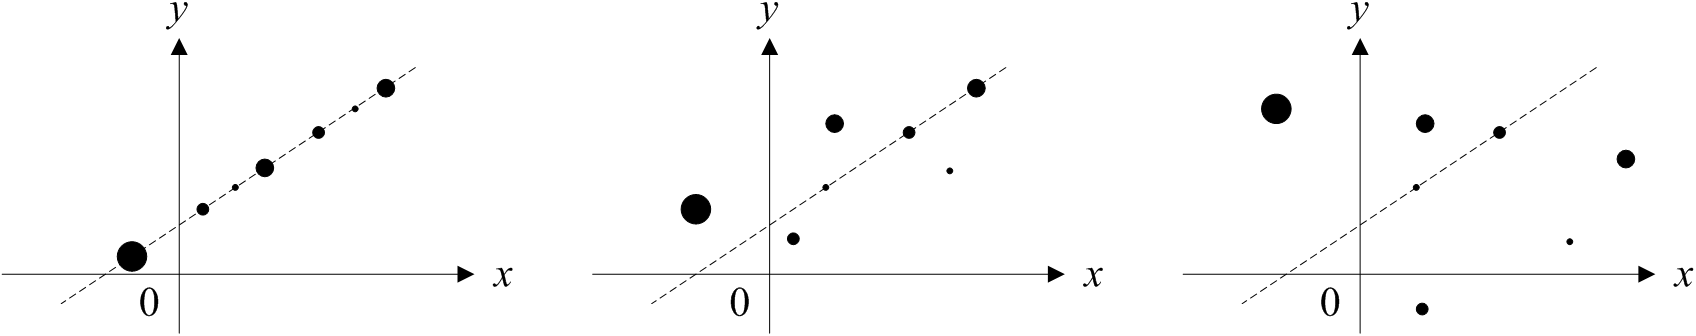
\includegraphics[height=2.2cm]{4.11.png}
\end{figure}

相关系数考察的就是这个关系。

首先引入线性代数的理论，令 $\hat{Y}=aX+b$，即$Y$在$X$上的投影：
\begin{align*}
e\left( a,b \right) &=E\left\{ \left[ Y-\left( aX+b \right) \right] ^2 \right\} \\
&=E\left( Y^2 \right) +a^2E\left( X^2 \right) +b^2-2aE\left( XY \right) -2bE\left( Y \right) +2abE\left( X \right)
\end{align*}

然后我们考察$X$需要做出怎么样的调整使得和$Y$的这个差异最小，即考察$e\left( a,b \right) $的极值。首先用一阶偏导求极值点$\left( a_0,b_0 \right) $：
\begin{align*}
&\begin{cases}
	\frac{\partial e}{\partial a}=2aE\left( X^2 \right) -2E\left( XY \right) +2bE\left( X \right) =0\\
	\frac{\partial e}{\partial b}=2b-2E\left( Y \right) +2aE\left( X \right) =0\\
\end{cases} \\
&\Rightarrow \begin{cases}
	a_0=\frac{\mathrm{Cov}\left( X,Y \right)}{D\left( X \right)}\\
	b_0=E\left( Y \right) -\frac{\mathrm{Cov}\left( X,Y \right)}{D\left( X \right)}\cdot E\left( X \right)\\
\end{cases}
\end{align*}
但这只是极值点，极大值还是极小值还是鞍点，需要考虑$e\left( a,b \right) $的Hessian矩阵的特征值：
\begin{align*}
&H\left( e \right) =\left[ \begin{matrix}
	\frac{\partial ^2e}{\partial a^2}&		\frac{\partial ^2e}{\partial a\partial b}\\
	\frac{\partial ^2e}{\partial b\partial a}&		\frac{\partial ^2e}{\partial b^2}\\
\end{matrix} \right] =\left[ \begin{matrix}
	2E\left( X^2 \right)&		2E\left( X \right)\\
	2E\left( X \right)&		2\\
\end{matrix} \right] \\
&\det \left[ H\left( e \right) \right] =4E\left( X^2 \right) -4\left[ 2E\left( X \right) \right] ^2=4D\left( X \right) >0
\end{align*}
再加上$\frac{\partial ^2e}{\partial a^2}=2E\left( X^2 \right) >0$，所以$\left( a_0,b_0 \right) $是极小值点，$e\left( a,b \right) $在该点有最小值：
\[
\left. e\left( a,b \right) \right|_{\left( a_0,b_0 \right)}=\left[ 1-\left( \frac{\mathrm{Cov}\left( X,Y \right)}{\sqrt{D\left( X \right)}\cdot \sqrt{D\left( Y \right)}} \right) ^2 \right] D\left( Y \right)
\]

上式衡量了$X$和$Y$在分布上的差异量，即 “努力地做出调整”后，$Y$和$X$的差异量。
若要考察一个已知的$Y$对$X_1$和$X_2$的线性关系谁大谁小，则需要排除$Y$的因素，于是我们可取前半部分因子
\[
\left[ 1-\left( \frac{\mathrm{Cov}\left( X_?,Y \right)}{\sqrt{D\left( X_? \right)}\cdot \sqrt{D\left( Y \right)}} \right) ^2 \right]
\]
该因子越小，说明差异量越小，和$X_?$的契合度越高。反之取平方项部分，记作$\rho _{XY}$
\[
\rho _{X_?Y}=\frac{\mathrm{Cov}\left( X_?,Y \right)}{\sqrt{D\left( X_? \right)}\cdot \sqrt{D\left( Y \right)}}
\]
$\rho _{X_?Y}$越大，说明和$X_?$的契合度越高。
也就是说，对于一个给定的$Y$和一堆$X_1,X_2,\cdots X_n$，我们可以用$\rho _{XY}$判断$Y$和某个$X_i$在分布上是最契合的，此时，$X_i$只需要做出调整$a_0X_i+b_0$就可以将差异减小到最小的程度。

对于现实的指导是，如果$\rho _{XY}$大到一定程度，我们就可以用关于$X$的一个简单的函数
\[
g\left( X \right) =\frac{\mathrm{Cov}\left( X,Y \right)}{D\left( X \right)}X+E\left( Y \right) -\frac{\mathrm{Cov}\left( X,Y \right)}{D\left( X \right)}\cdot E\left( X \right)
\]
代替$Y$考察分布。
比如对于正态分布，有很多很好很简单的性质，我们也有很多统计手段和公式。
倘若 “很像”正态分布，那我们就可以用正态分布代替$Y$，进而可以通过公式用标准分布计算，整个问题就变得简单明了。

%============================================================
\subsection{相关的几何意义}

$\rho _{XY}$表示的相关性如下图。
可见，当$\rho _{XY}=\pm 1$时，$Y\ne aX+b$的地方概率为0，$f\left( x,y \right) $将由一张三维曲面退化成一个二维平面。

\begin{figure}[h]
\centering
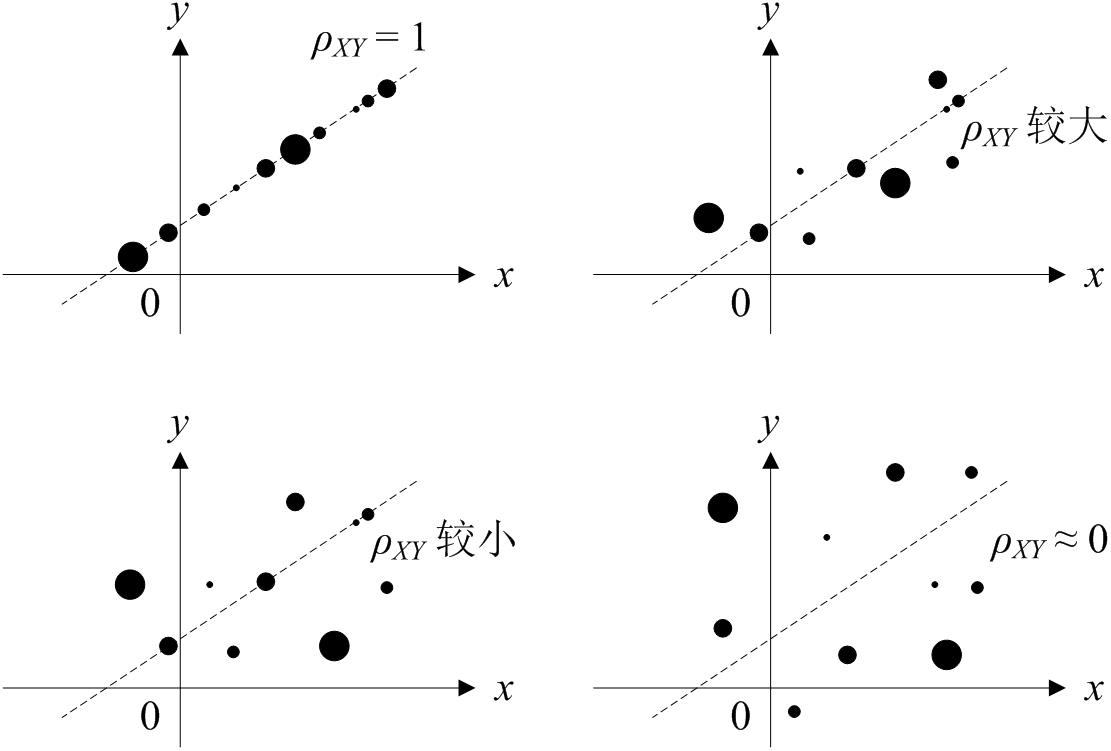
\includegraphics[height=4.5cm]{4.12.png}
\end{figure}

以二维正态分布为例：
\begin{align*}
&\left( X,Y \right) \sim N\left( \mu _1,\mu _2,{\sigma _1}^2,{\sigma _2}^2,\rho \right) \\
&f\left( x,y \right) =\frac{1}{2\pi \sigma _1\sigma _2\sqrt{1-\rho ^2}}e^{-\frac{1}{2\left( 1-\rho ^2 \right)}\left[ \frac{\left( x-\mu _1 \right) ^2}{{\sigma _1}^2}-2\rho \frac{\left( x-\mu _1 \right) \left( y-\mu _2 \right)}{\sigma _1\sigma _2}+\frac{\left( y-\mu _2 \right) ^2}{{\sigma _2}^2} \right]} \\
&\rho \in \left( -1,1 \right)
\end{align*}
$\rho $表示了$X,Y$的相关性，当$\rho =0.99$时，$f\left( x,y \right) $几乎成为一个平面。

\begin{figure}[h]
\centering
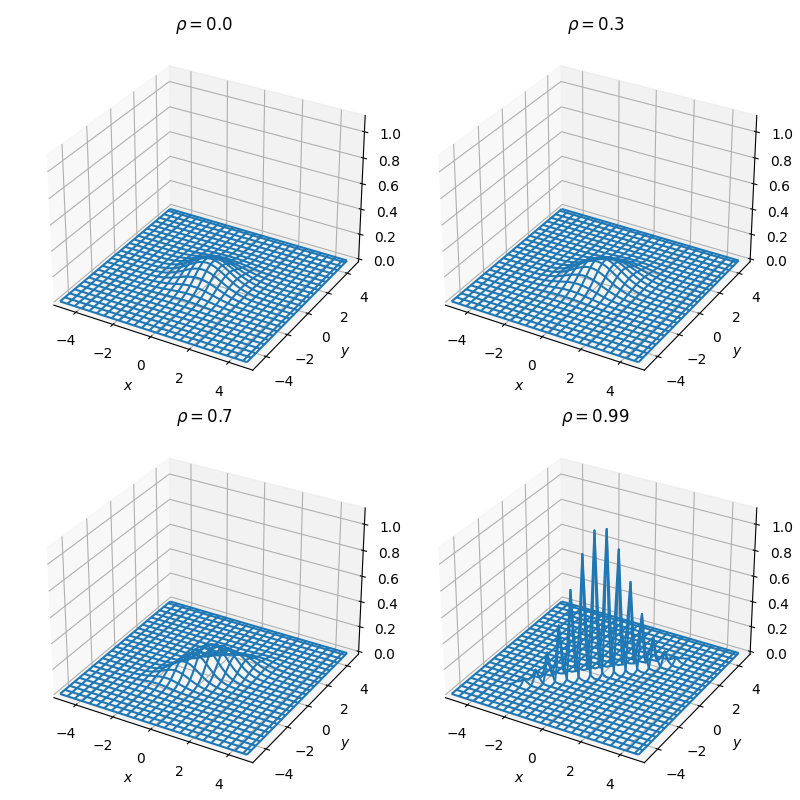
\includegraphics[height=8cm]{4.13.png}
\end{figure}

\begin{tcolorbox}
可见，相关描述了密度函数的扁平性，相关系数就是这个扁平性的量化指标，$\rho _{XY}$越大，曲面$f\left( x,y \right) $越趋于平面。
\end{tcolorbox}

%============================================================
\subsection{协方差和相关系数的线性代数意义}

参考线性代数中向量的柯西—施瓦茨不等式的表述。若$\boldsymbol{x},\boldsymbol{y}$为内积空间$V$中的两个向量，则必有：
\[
\left| \left< \boldsymbol{x},\boldsymbol{y} \right> \right|\leqslant \sqrt{\left< \boldsymbol{x},\boldsymbol{x} \right>}\sqrt{\left< \boldsymbol{y},\boldsymbol{y} \right>}
\]
当且仅当$\boldsymbol{x}=0$或$\boldsymbol{y}=0$或$\boldsymbol{x}=\boldsymbol{y}=0$或$\boldsymbol{x},\boldsymbol{y}$线性相关时等号成立。
于是当$\boldsymbol{x}\ne \boldsymbol{y}$时，我们可以用柯西—施瓦茨不等式定义它们的夹角：
\[
\cos \theta =\frac{\left< \boldsymbol{x},\boldsymbol{y} \right>}{\sqrt{\left< \boldsymbol{x},\boldsymbol{x} \right>}\sqrt{\left< \boldsymbol{y},\boldsymbol{y} \right>}}
\]
对比观察得到，协方差就是两个向量的内积，相关系数就是它们的夹角的余弦：
\[
\rho _{XY}=\frac{\mathrm{Cov}\left( X,Y \right)}{\sqrt{DX}\cdot \sqrt{DY}}=\frac{\mathrm{Cov}\left( X,Y \right)}{\sqrt{\mathrm{Cov}\left( X,X \right)}\cdot \sqrt{\mathrm{Cov}\left( Y,Y \right)}}
\]
各部分对应关系如下：
\[
\begin{array}{l}
	\mathrm{Cov}\left( , \right)\\
	X\\
	Y\\
	DX\\
	DY\\
	\mathrm{Cov}\left( X,Y \right)\\
	\rho _{XY}\\
\end{array} \quad \leftrightarrow \quad \begin{array}{l}
	\left< , \right>\\
	\boldsymbol{x}\\
	\boldsymbol{y}\\
	\left< \boldsymbol{x},\boldsymbol{x} \right>\\
	\left< \boldsymbol{y},\boldsymbol{y} \right>\\
	\left< \boldsymbol{x},\boldsymbol{y} \right>\\
	\cos \theta\\
\end{array}
\]

更进一步，将一维随机变量的分布视为向量，则所有分布的集合可以视作向量空间$V$，任取两种分布$X,Y$用向量记号记作$\boldsymbol{x},\boldsymbol{y}$，我们采用协方差作为操作，即$\left< , \right> =\mathrm{Cov}\left( , \right) $，必然满足内积的4个要求：
\begin{enumerate}[label=\Roman*.]
    \item 正定性，$\left< \boldsymbol{x},\boldsymbol{x} \right> \geqslant 0$，当且仅当$\boldsymbol{x} =0$（即常数分布）时等号成立；
    \item $\left< \alpha \boldsymbol{x},\boldsymbol{y} \right> =\alpha \left< \boldsymbol{x},\boldsymbol{y} \right> $；
    \item 交换律，$\left< \boldsymbol{x},\boldsymbol{y} \right> =\left< \boldsymbol{y},\boldsymbol{x} \right> $；
    \item 分配律，$\left< \boldsymbol{x}+\boldsymbol{y},\boldsymbol{z} \right> =\left< \boldsymbol{x},\boldsymbol{z} \right> +\left< \boldsymbol{y},\boldsymbol{z} \right> $。
\end{enumerate}
其中I、II、III这3条从数学期望的定义式就可得
IV证明如下：
\begin{align*}
&\mathrm{Cov}\left( \left( X+Y \right) ,Z \right) =E\left[ \left( X+Y-E\left( X+Y \right) \right) \left( Z-EZ \right) \right] \\
&=E\left[ \left( X+Y+EX+EY \right) \left( Z-EZ \right) \right] \\
&=E\left( XZ-XEZ+YZ-YEZ+ZEX-EXEZ+ZWY-EZEY \right) \\
&=E\left( XZ \right) +E\left( YZ \right) -E\left( EXEZ \right) -E\left( EZEY \right) \\
&=\mathrm{Cov}\left( X,Z \right) +\mathrm{Cov}\left( Y,Z \right)
\end{align*}

\begin{tcolorbox}
可见，一维随机变量连同协方差运算构成了内积空间，常数分布是零向量，$\rho _{XY}$表示了两个向量的夹角的余弦。
\end{tcolorbox}

%============================================================
\subsection{方差与范数}

更“线性代数化地说”，方差是变量的一个范数的算术平方$DX\leftrightarrow \left\| \boldsymbol{x} \right\| ^2$。范数的要求如下：
\begin{itemize}
    \item 正定性，$\left\| \boldsymbol{x} \right\| \geqslant 0$，当且仅当$\boldsymbol{x}=0$时，等号成立；
    \item $\left\| \alpha \boldsymbol{x} \right\| =\left| \alpha \right|\left\| \boldsymbol{x} \right\| $；
    \item 三角不等式，$\left\| \boldsymbol{x}+\boldsymbol{y} \right\| \leqslant \left\| \boldsymbol{x} \right\| +\left\| \boldsymbol{y} \right\| $。
\end{itemize}
对应方差的性质：
\begin{itemize}
    \item $D\left( X \right) \geqslant 0$，当且仅当$P\left\{ X=EX \right\} =1$时等号成立。
    \item $D\left( kX \right) =k^2\cdot D\left( X \right) $
    \item $D\left( X+Y \right) =DX+DY+2\mathrm{Cov}\left( X,Y \right) $
\end{itemize}

%============================================================
\subsection{例}

\begin{example}
继续第三章中的例子，若5个产品中有2个次品，每次抽取一个，取两次，记$X$表示第一次取到次品的个数，$Y$表示第二次取到次品的个数，讨论：
\begin{enumerate}
    \item 不放回抽取的情况下，
    \item 放回抽取的情况下，
\end{enumerate}
这两种情况下，$X,Y$的协方差。
\end{example}

解：

由题干可得，$X,Y$取值只可能是0或1。

1. 不放回抽取的情况下的分布律$p_{ij}$：
\[
\begin{matrix}
	&		0&		1&		p_{\cdot j}\\
	0&		\frac{3}{10}&		\frac{3}{10}&		\frac{3}{5}\\
	1&		\frac{3}{10}&		\frac{1}{10}&		\frac{2}{5}\\
	p_{i\cdot}&		\frac{3}{5}&		\frac{2}{5}&		1\\
\end{matrix}
\]
\begin{align*}
&\because \begin{cases}
	E\left( XY \right) =0\cdot 0\cdot \frac{3}{10}+0\cdot 1\cdot \frac{3}{10}+1\cdot 0\cdot \frac{3}{10}+1\cdot 1\cdot \frac{1}{10}=\frac{1}{10}\\
	E\left( X \right) =0\cdot \frac{3}{5}+1\cdot \frac{2}{5}=\frac{2}{5}\\
	E\left( Y \right) =0\cdot \frac{3}{5}+1\cdot \frac{2}{5}=\frac{2}{5}\\
\end{cases} \\
&\therefore \mathrm{Cov}\left( X,Y \right) =E\left( XY \right) -E\left( X \right) \cdot E\left( Y \right) =\frac{1}{10}-\frac{4}{25}=-\frac{3}{50}
\end{align*}

2. 放回抽取的情况下的分布律$p_{ij}$：
\[
\begin{matrix}
	&		0&		1&		p_{\cdot j}\\
	0&		\frac{9}{25}&		\frac{6}{25}&		\frac{3}{5}\\
	1&		\frac{6}{25}&		\frac{4}{25}&		\frac{2}{5}\\
	p_{i\cdot}&		\frac{3}{5}&		\frac{2}{5}&		1\\
\end{matrix}
\]
\begin{align*}
&\because \begin{cases}
	E\left( XY \right) =0\cdot 0\cdot \frac{9}{25}+0\cdot 1\cdot \frac{6}{25}+1\cdot 0\cdot \frac{6}{25}+1\cdot 1\cdot \frac{4}{25}=\frac{4}{25}\\
	E\left( X \right) =0\cdot \frac{3}{5}+1\cdot \frac{2}{5}=\frac{2}{5}\\
	E\left( Y \right) =0\cdot \frac{3}{5}+1\cdot \frac{2}{5}=\frac{2}{5}\\
\end{cases} \\
&\therefore \mathrm{Cov}\left( X,Y \right) =E\left( XY \right) -E\left( X \right) \cdot E\left( Y \right) =\frac{4}{25}-\frac{4}{25}=0
\end{align*}

\begin{tcolorbox}
从该题解读协方差的意义。在(2)放回的情况下，从事实角度出发，$X,Y$是独立的，既然独立就没有任何关系，包括线性关系，自然$\mathrm{Cov}\left( X,Y \right) =0$。
在(1)不放回的情况下，第一次抽中次品时，是不利于再次抽中次品这个事件的发生的。
\end{tcolorbox}






\newpage
\section{矩和协方差矩阵}

本节简单介绍矩和协方差矩阵的概念。

本节要点：
\begin{itemize}
    \item 了解矩的概念；
    \item 了解协方差矩阵的概念。
\end{itemize}

%============================================================
\subsection{矩的概念}

\begin{definition}[矩]
设一维随机变量$X$，若对于$k\in \mathbb{Z} ^+$，$E\left[ \left( X-c \right) ^k \right] $存在，则称其为{\bf $X$关于$c$点的$k$阶矩}。
特别地，当$c=0$时，称$E\left( X^k \right) $为{\bf $X$的$k$阶原点矩}，当$c=EX$时，称$E\left[ \left( X-EX \right) ^k \right] $为{\bf $X$的$k$阶中心矩}。
\end{definition}

显然：
\begin{itemize}
    \item $X$的1阶原点矩即为数学期望，$EX$；
    \item $X$的1阶中心矩总是为0，$E\left( X-EX \right) =0$；
    \item $X$的2阶中心矩即为方差，$DX$。
\end{itemize}

\begin{definition}[混合矩]
设二维随机变量$\left( X,Y \right) $，若对于$k,l\in \mathbb{Z} ^+$，$E\left( X^kY^l \right) $存在，则称其为{\bf $X,Y$的$k+l$阶混合原点矩}；
若对于$k,l\in \mathbb{Z} ^+$，数学期望$E\left[ \left( X-EX \right) ^k\left( Y-EY \right) ^l \right] $存在，则称其为{\bf $X,Y$的$k+l$阶混合中心矩}。
\end{definition}

显然：
\begin{itemize}
    \item $X,Y$的1+1阶混合中心矩即为它们的协方差，$\mathrm{Cov}\left( X,Y \right) $。
\end{itemize}

\begin{tcolorbox}
1阶矩和2阶矩用得较多，3、4阶用的较少。
3、4阶能引出“偏度系数”和“峰度系数”，详见“教材\cite{book2}”P122～123。
广义上来讲，矩也是数字特征，但在实际使用中，数字特征往往特指期望、方差、协方差。
\end{tcolorbox}

%============================================================
\subsection{协方差矩阵的概念}

\begin{definition}[协方差矩阵]
设$n$维随机变量$\left( X_1,X_2,\cdots ,X_n \right) $，记它们随意两两组合的协方差为$c_{ij}$，即：
\[
c_{ij}:=\mathrm{Cov}\left( X_i,X_j \right)
\]
若$c_{ij}$总是存在，则称它们组成的矩阵为{\bf $\left( X_1,X_2,\cdots ,X_n \right) $的协方差矩阵}，记作$\mathbf{C}$，即：
\[
\mathbf{C}:=\left[ \begin{matrix}
	c_{11}&		c_{12}&		\cdots&		c_{1n}\\
   	c_{21}&		c_{22}&		\cdots&		c_{2n}\\
   	\vdots&		\vdots&		&		\vdots\\
   	c_{n1}&		c_{n2}&		\cdots&		c_{nn}\\
\end{matrix} \right]
\]
\end{definition}

显然$\mathbf{C}$是一个实对称方阵，其对角线为每个变量的方差。






\newpage
\section{本章小结}

本章介绍了随机变量的数字特征：
\begin{itemize}
    \item 对于一个变量，有：数学期望、方差，描述了变量的分布情况；
    \item 对于两个变量，有：协方差、相关系数，描述了样本点$\left\{ X=x_i,Y=y_j \right\} $的分布是否趋于直线。
\end{itemize}

~

数学期望定义公式
\begin{align*}
&EX:=\sum_i{x_i\cdot p_i} \\
&EX:=\int_{-\infty}^{+\infty}{xf\left( x \right) \cdot dx}
\end{align*}

方差定义公式和便捷公式
\begin{align*}
&DX:=E\left[ \left( X-EX \right) ^2 \right] \\
&DX=E\left( X^2 \right) -\left( EX \right) ^2
\end{align*}

协方差定义公式和便捷公式
\begin{align*}
&\mathrm{Cov}\left( X,Y \right) :=E\left[ \left( X-EX \right) \left( Y-EY \right) \right] \\
&\mathrm{Cov}\left( X,Y \right) =E\left( XY \right) -EX\cdot EY
\end{align*}

相关系数定义公式和便捷公式
\begin{align*}
&\rho _{XY}:=\frac{\mathrm{Cov}\left( X,Y \right)}{\sqrt{DX}\cdot \sqrt{DY}} \\
&\rho _{XY}=\frac{E\left( XY \right) -EX\cdot EY}{\sqrt{E\left( X^2 \right) -\left( EX \right) ^2}\cdot \sqrt{E\left( Y^2 \right) -\left( EY \right) ^2}}
\end{align*}

数学期望的性质
\begin{align*}
&E\left( c \right) =c \\
&X\geqslant a\Rightarrow EX\geqslant a,X\leqslant a\Rightarrow EX\leqslant a \\
&E\left( kX \right) =k\cdot E\left( X \right) \\
&E\left( kX+c \right) =k\cdot E\left( X \right) +c \\
&E\left( X\pm Y \right) =E\left( X \right) \pm E\left( Y \right) \\
&\text{若}X,Y\text{相互独立}\Rightarrow E\left( XY \right) =E\left( X \right) \cdot E\left( Y \right) \\
&\left[ E\left( XY \right) \right] ^2\leqslant E\left( X^2 \right) \cdot E\left( Y^2 \right)
\end{align*}

方差的性质
\begin{align*}
&D\left( c \right) =0 \\
&D\left( X \right) \geqslant 0, \text{当且仅当}P\left\{ X=EX \right\} =1\text{时等号成立} \\
&D\left( kX \right) =k^2\cdot D\left( X \right) \\
&D\left( kX+c \right) =k^2\cdot D\left( X \right) \\
&\text{若}X,Y\text{相互独立}\Rightarrow D\left( X\pm Y \right) =D\left( X \right) +D\left( Y \right)
\end{align*}

协方差的性质
\begin{align*}
&\mathrm{Cov}\left( X,X \right) =DX \\
&D\left( X\pm Y \right) =DX+DY\pm 2\mathrm{Cov}\left( X,Y \right) \\
&\mathrm{Cov}\left( X,c \right) =0 \\
&\mathrm{Cov}\left( X,Y \right) =\mathrm{Cov}\left( Y,X \right) \\
&\mathrm{Cov}\left( aX,bY \right) =ab\mathrm{Cov}\left( X,Y \right) \\
&\mathrm{Cov}\left( X_1\pm X_2,Y \right) =\mathrm{Cov}\left( X_1,Y \right) \pm \mathrm{Cov}\left( X_2,Y \right) \\
&\left[ \mathrm{Cov}\left( X,Y \right) \right] ^2\leqslant DX\cdot DY
\end{align*}

相关系数的性质
\begin{align*}
&\rho _{XY}\in \left[ -1,1 \right] \\
&X\text{和}Y\text{成线性关系}\Leftrightarrow \rho _{XY}=\pm 1 \\
&\rho _{\left( aX \right) \left( bY \right)}=\begin{cases}
	\rho _{XY},&		ab>0\\
	-\rho _{XY},&		ab<0\\
\end{cases}
\end{align*}

~

数字特征的物理意义和线性代数意义：
\begin{table}[h]
\centering
\begin{tabular}{lll}
    \toprule
    数字特征 & 物理意义/线性代数意义 & 量纲\\
    \midrule
    数学期望 & 质心位置 & $\left[ \mathrm{m} \right] $\\
    方差 & 单位质量的转动惯量，范数 & $\left[ \mathrm{m}^2 \right] $\\
    协方差 & 两个向量的内积 & $\left[ \mathrm{m}^2 \right] $\\
    相关系数 & 两个向量的夹角的余弦 & 无量纲\\
    \bottomrule
\end{tabular}
\end{table}

学习概率论中的数字特征，要特别注意它们的物理意义和几何意义，用其他学科的知识点相互印证，加深对这些概念的理解。










\chapter{大数定理和中心极限定理}

本章简单介绍概率论中两大定理——大数定理和中心极限定理，作为概率论的终结。

本章要点：
\begin{itemize}
    \item 大数定理。
    \item 中心极限定理。
\end{itemize}

\newpage
\section{大数定理}

本节介绍大数定理。
大数定理描述了随着试验次数的增加，发生频率稳定趋于概率这一现象。

本节要点：
\begin{itemize}
    \item 掌握均值的概念；
    \item 掌握依概率收敛的概念；
    \item 深刻理解3个大数定理的意义；
    \item 深刻理解辛钦大数定理的证明过程。
\end{itemize}

%============================================================
\subsection{均值的概念}

\begin{definition}[均值]
设随机试验$E$对应有一维随机变量$X$，若进行一轮$n$次重复试验，得到一组随机变量的值的序列，暂记作$X_1,X_2,\cdots ,X_n$，其中$X_i$表示该轮第$i$次试验得到的值，则称它们的算术平均为{\bf 该组序列的均值}，记作$\bar{X}$，即：
\[
\bar{X}:=\frac{1}{n}\sum_{i=1}^n{X_i}
\]
\end{definition}

由于每轮试验都会得到一组不同的序列，加之每轮的$n$的取值又可以不同，所以$\bar{X}$的取值在每轮试验后都会不同，$\bar{X}$符合随机变量的定义要求，它也是一个随机变量。
本节的大数定理就是在不知道$\bar{X}$的分布的情况下，考察当$n\rightarrow \infty $时$\bar{X}$的趋近值。

%============================================================
\subsection{依概率收敛的概念}

\begin{definition}[依概率收敛]
设一组随机变量组成的序列$Z_1,Z_2,\cdots ,Z_n,\cdots $，若存在常数$a$，使得$\forall \varepsilon >0$，有：
\[
\underset{n\rightarrow \infty}{\lim}P\left\{ \left| Z_n-a \right|<\varepsilon \right\} =1
\]
则称{\bf 该序列依概率收敛于$a$}，记作：
\[
\underset{n\rightarrow \infty}{\lim}Z_n\overset{P}{=}a
\]
\end{definition}

注意，依概率收敛不同于微积分中的极限：
\begin{itemize}
    \item 首先，依概率收敛的意思是随着$n$的增大，$Z_n$的分布越来越向$a$集中，最后$Z_n$只出现在$a$；
    \item 其次，收敛要求按照概率$P$，而非形如微积分中的$\underset{n\rightarrow \infty}{\lim}Z_n=a$，所以写作$\underset{n\rightarrow \infty}{\lim}Z_n\overset{P}{=}a$。
\end{itemize}

~

以掷硬币为例，设进行一轮只投掷1次的试验，得到的均值记作$\bar{X}_1$，再进行一轮投掷2次的试验，得到的均值记作$\bar{X}_2$，以此类推，将投掷$n$次的那一轮试验得到的均值记作$\bar{X}_n$。
则随着投掷次数的增多，$\bar{X}_n$将会趋向0.5，用上述的数学表达式可写为：
\[
\underset{n\rightarrow \infty}{\lim}\bar{X}_n\overset{P}{=}\frac{1}{2}
\]

%============================================================
\subsection{引理}

\begin{lemma}[马尔可夫不等式]
设有一维随机变量$X$，若取值非负，则$\forall \varepsilon >0$，必有：
\[
P\left\{ X\geqslant \varepsilon \right\} \leqslant \frac{EX}{\varepsilon}
\]
\end{lemma}

\begin{proof}
以连续变量为例，由于$X$取值非负，则$\left. f\left( x \right) \right|_{x<0}=0$，于是：
\begin{align*}
P\left\{ X\geqslant \varepsilon \right\} &=\int_{\varepsilon}^{+\infty}{f\left( x \right) \cdot dx}\leqslant \int_{\varepsilon}^{+\infty}{\frac{x}{\varepsilon}\cdot f\left( x \right) \cdot dx} \\
&=\frac{1}{\varepsilon}\cdot \int_{\varepsilon}^{+\infty}{xf\left( x \right) \cdot dx}\leqslant \frac{1}{\varepsilon}\cdot \int_0^{+\infty}{xf\left( x \right) \cdot dx} \\
&=\frac{1}{\varepsilon}\cdot EX
\end{align*}
\end{proof}

\begin{lemma}[切比雪夫不等式]
设有一维随机变量$X$有期望$EX$和方差$DX$，则$\forall \varepsilon >0$，必有：
\[
P\left\{ \left| X-EX \right|\geqslant \varepsilon \right\} \leqslant \frac{DX}{\varepsilon ^2}
\]
或
\[
P\left\{ \left| X-EX \right|<\varepsilon \right\} \geqslant 1-\frac{DX}{\varepsilon ^2}
\]
\end{lemma}

\begin{proof}
以连续变量为例，注意到$P\left\{ \left| X-EX \right|\geqslant \varepsilon \right\} =P\left\{ \left( X-EX \right) ^2\geqslant \varepsilon ^2 \right\} $，且无论$X$如何取值，$\left( X-EX \right) ^2$取值必然非负，利用马尔可夫不等式，有：
\[
P\left\{ \left| X-EX \right|\geqslant \varepsilon \right\} =P\left\{ \left( X-EX \right) ^2\geqslant \varepsilon ^2 \right\} \leqslant \frac{E\left[ \left( X-EX \right) ^2 \right]}{\varepsilon ^2}=\frac{DX}{\varepsilon ^2}
\]
\end{proof}

这两个不等式反映了所有分布所遵循的特征。
切比雪夫不等式的第二个表达式更容易反映出其意义。无论$X$是什么分布，以中心$EX$的范围$\varepsilon $，范围越小，概率越小。同样的范围$\varepsilon $，若概率分布越分散，即$DX$越大，则该范围内的概率越小。

%============================================================
\subsection{大数定理}

\begin{theorem}[伯努利大数定理]
设有$n$重伯努利试验，事件$A$的发生概率为$p$，令$X_i=1$表示在第$i$次试验中事件$A$发生，$X_i=0$表示在第$i$次试验中事件$A$不发生，$\bar{X}=\frac{1}{n}\sum_{i=1}^n{X_i}$表示在一共$n$次试验中事件$A$的发生均值，则当$n\rightarrow +\infty $时，$\bar{X}$依概率收敛于事件$A$的发生概率，即：
\[
\underset{n\rightarrow \infty}{\lim}\bar{X}\overset{P}{=}p
\]
\end{theorem}

\begin{proof}
这里我们已知每次子试验为一个二项试验，虽然我们不知道$\bar{X}$的分布规律，但我们可以通过考察$\bar{X}$的表达式，用切比雪夫不等式判断它落入$p$附近的概率。由$n$次试验相互独立可得：
\begin{align*}
&\because \bar{X}=\frac{1}{n}\sum_{i=1}^n{X_i} \\
&\therefore \begin{cases}
	E\bar{X}=\frac{1}{n}\sum_{i=1}^n{EX_i}=p\\
	D\bar{X}=\frac{1}{n^2}\sum_{i=1}^n{DX_i}=\frac{p\left( 1-p \right)}{n}\\
\end{cases}
\end{align*}
带入切比雪夫不等式，并两边取极限：
\begin{align*}
&\because P\left\{ \left| \bar{X}-p \right|<\varepsilon \right\} \geqslant 1-\frac{p\left( 1-p \right)}{\varepsilon ^2n} \\
&\therefore \underset{n\rightarrow +\infty}{\lim}P\left\{ \left| \bar{X}-p \right|<\varepsilon \right\} \geqslant \underset{n\rightarrow +\infty}{\lim}\left[ 1-\frac{p\left( 1-p \right)}{\varepsilon ^2n} \right] =1
\end{align*}
作为概率$P\left\{  \right\} \leqslant 1$，由夹逼定理得：
\[
\underset{n\rightarrow \infty}{\lim}P\left\{ \left| \bar{X}-p \right|<\varepsilon \right\} =1
\]
\end{proof}

伯努利大数定理表示随着试验次数的增加，事件$A$的发生频率趋于概率，为概率的统计定义给出了理论保障。

从证明过程看，关键因素是$D\bar{X}=\frac{1}{n^2}\sum_{i=1}^n{DX_i}$，该等式成立的前提是$X_i$相互独立，这点由伯努利试验的特点保证。

\begin{theorem}[辛钦大数定理]
设$X_1,X_2,\cdots ,X_n,\cdots $为独立同分布的随机变量，若它们都有相同的数学期望和方差，暂记数学期望为$\mu $，则有：
\[
\underset{n\rightarrow \infty}{\lim}\bar{X}\overset{P}{=}\mu
\]
\end{theorem}

\begin{proof}
还是利用切比雪夫不等式，从$\bar{X}$的表达式入手：
\begin{align*}
&\because \bar{X}=\frac{1}{n}\sum_{i=1}^n{X_i} \\
&\therefore \begin{cases}
	EZ=E\left( \frac{1}{n}\sum_{i=1}^n{X_i} \right) =\frac{1}{n}\sum_{i=1}^n{E\left( X_i \right)}=\frac{n\cdot \mu}{n}=\mu\\
	DZ=D\left( \frac{1}{n}\sum_{i=1}^n{X_i} \right) =\frac{1}{n^2}\sum_{i=1}^n{D\left( X_i \right)}=\frac{\sigma ^2}{n}\\
\end{cases}
\end{align*}
带入切比雪夫不等式，并两边取极限：
\begin{align*}
&\because P\left\{ \left| \bar{X}-\mu \right|<\varepsilon \right\} \geqslant 1-\frac{\sigma ^2}{\varepsilon ^2n} \\
&\therefore \underset{n\rightarrow +\infty}{\lim}P\left\{ \left| \bar{X}-\mu \right|<\varepsilon \right\} \geqslant \underset{n\rightarrow +\infty}{\lim}\left[ 1-\frac{\sigma ^2}{\varepsilon ^2n} \right] =1
\end{align*}
夹逼定理，后略。
\end{proof}

辛钦大数定理反映了任意一种随机试验在重复大量次数后，均值趋于期望。
伯努利大数定理是它的一个特例。

从证明过程看，关键因素依然是$DZ=\frac{1}{n^2}\sum_{i=1}^n{D\left( X_i \right)}$，也即随机变量需要独立。

\begin{theorem}[切比雪夫大数定理]
设$X_1,X_2,\cdots ,X_n,\cdots $为独立随机变量，若它们都有各自的数学期望和方差，暂记数学期望为$\mu _i$，则有：
\[
\underset{n\rightarrow \infty}{\lim}\bar{X}\overset{P}{=}\frac{1}{n}\sum_{i=1}^n{\mu _i}
\]
\end{theorem}

证明思路同上，略。

%============================================================
\subsection{大数定理的说明}

广义上来讲，一切描述“独立试验”中$n\rightarrow \infty $时均值$\bar{X}$的极限的定理都是大数定理。

伯努利大数定理最初限定在$n$重伯努利试验，论述$n\rightarrow \infty $时事件$A$的发生频率趋于概率。但可以放宽到有相同分布的独立变量，此时就是辛钦大数定理，在“教材\cite{book2}”中称为伯努利大数定理。如果进一步放宽条件到只要求相互独立，并不同分布，则是切比雪夫大数定理。

大数定理体现的是“随着样本的增加，发生频率稳定趋于概率”这一人类经验认识，所以有时也被称为“大数定律”。

%============================================================
\subsection{例}

\begin{example}
设$X$为一未知的一维随机变量，已知有期望和方差$\mu ,\sigma ^2$，分析$X$落在以$\left( \mu -3\sigma ,\mu +3\sigma \right) $内的概率。
\end{example}

解：

根据切比雪夫不等式，有：
\[
P\left\{ \left| X-\mu \right|<3\sigma \right\} \geqslant 1-\frac{\sigma ^2}{\left( 3\sigma \right) ^2}=1-\frac{1}{9}=0.889
\]
$X$落在以$\left( \mu -3\sigma ,\mu +3\sigma \right) $内的概率大于0.889。

~

\begin{example}
设$X$为一未知的一维随机变量，若能将其标准化为$X^*$，分析$X^*$落在以$\left( -2,2 \right) $内的概率。
\end{example}

解：

由于$X^*$是标准化的随机变量，于是$E\left( X^* \right) =0,D\left( X^* \right) =1$，可得：
\[
P\left\{ \left| X^*-E\left( X^* \right) \right|<2 \right\} \geqslant 1-\frac{D\left( X^* \right)}{2^2}=\frac{3}{4}
\]
$X^*$落在以$\left( -2,2 \right) $内的概率大于$3/4$。






\newpage
\section{中心极限定理}

本节介绍中心极限定理。
中心极限定理描述了随着试验次数的增加，所有试验结果的值的累计趋于正态分布这一现象。

本节要点：
\begin{itemize}
    \item 理解列维—林德伯格中心极限定理。
\end{itemize}

%============================================================
\subsection{列维—林德伯格中心极限定理}

\begin{theorem}[列维—林德伯格中心极限定理]
设$X_1,X_2,\cdots ,X_n,\cdots $为独立同分布的随机变量，若它们都有相同的数学期望和方差，分别记为$\mu ,\sigma ^2$，有：
\[
\underset{n\rightarrow \infty}{\lim}P\left\{ \frac{X_1+X_2+\cdots +X_n-n\mu}{\sqrt{n}\sigma}\leqslant x \right\} =\varPhi \left( x \right) =\frac{1}{\sqrt{2\pi}}\int_{-\infty}^x{e^{-\frac{t^2}{2}}dt}
\]
即当$n\rightarrow \infty $时，$\frac{X_1+X_2+\cdots +X_n-n\mu}{\sqrt{n}\sigma}$服从标准分布。
\end{theorem}

列维—林德伯格中心极限定理告诉我们，若有一系列独立同分布的随机变量，倘若将它们相加后再做标准化：
\[
\begin{cases}
	Y=X_1+X_2+\cdots +X_n\\
	EY=n\mu\\
	DY=n\sigma ^2\\
\end{cases}\Rightarrow Y^*=\frac{Y-EY}{\sqrt{DY}}=\frac{Y-n\mu}{\sqrt{n}\sigma}
\]
则当$n\rightarrow \infty $时$Y^*\sim N\left( 0,1 \right) $，也即$Y\sim N\left( n\mu ,n\sigma ^2 \right) $。
实际中，一般$n\geqslant 30$时，我们就可以认为$X_1,X_2,\cdots ,X_n$的叠加服从正态分布，即：
\[
\sum_{i=1}^n{X_i}\sim N\left( n\mu ,n\sigma ^2 \right)
\]

中心极限定理更重要的实际意义在于告诉我们，$X_1,X_2,\cdots ,X_n$只需要独立同分布就行，具体是什么分布并不重要，可以是任意的、未知的、或者不可表达式化的，甚至它们之间允许有略微的非独立，只要$n$够大，它们的叠加就可以看成正态分布。

%============================================================
\subsection{中心极限定理的说明}

除了列维—林德伯格中心极限定理，还有棣莫弗—拉普拉斯中心极限定理等。
中心极限定理是当$n$足够大时叠加可以看成正态分布的一系列定理的统称。
中心极限定理依然要求“独立试验”。

%============================================================
\subsection{例}

\begin{example}
设有200台独立工作的设备，每台设备的故障概率为1/200，如果出现故障，只需一名维修工即可修复，试分析需要多少维修工才能使出现故障无法及时修理的概率控制在0.03以内。
\end{example}

解：

分析，由于一台故障设备只需一名维修工修复，所以问题就成为这200台设备同时有几台及以上同时发生故障的概率$<3\%$，也即这200台设备同时有几台及以下同时发生故障的概率$\geqslant 97\%$。

1. 设备故障可以视作0-1分布且$p=1/200$，令记$X_i=1$表示第$i$台设备出现故障，则$X_i$服从0-1分布，即
\begin{align*}
&X_i\sim B\left( 1,p \right) \\
&p=\frac{1}{200} \\
&\mu =EX_i=p=\frac{1}{200} \\
&\sigma ^2=DX_i=p\left( 1-p \right) =\frac{199}{200\cdot 200}
\end{align*}

2. 令$Y=\sum{X_i}$，即表示200台设备中同时故障的台数，$Y$也是随机变量，于是根据列维—林德伯格中心极限定理，$Y$服从正态分布$N\left( n\mu ,n\sigma ^2 \right) $：
\[
Y\sim N\left( n\mu ,n\sigma ^2 \right) \overset{n=200}{=}N\left( 1,\frac{199}{200} \right)
\]

3. 根据正态分布和标准正态分布的关系，$y$及$y$台以下同时故障的概率：
\[
P\left\{ Y\leqslant y \right\} =\varPhi \left( \frac{y-\mu}{\sigma} \right) =\varPhi \left( \frac{y-1}{\sqrt{199/200}} \right) \geqslant 97\%
\]

4. 查表得$\varPhi \left( 1.88 \right) \approx 0.97$，即$P\left\{ Y\leqslant 2.88 \right\} =0.97$，说明3台及3台以下设备同时故障的概率占了97\%以上，因此只要配备3个维修工即可。

解二：
也可以用泊松分布，令$X$为同时故障的台数，服从泊松分布：
\[
P\left\{ X=x \right\} =\frac{\lambda ^x}{x!}e^{-\lambda},\quad \lambda =200\cdot \frac{1}{200}=1
\]
$n$台及$n$以下同时故障的概率：
\[
P\left\{ X\leqslant n \right\} =\sum_{x=0}^n{\frac{1}{x!}e^{-1}}
\]
计算$n=1,2,3,4$得：
\begin{align*}
&P\left\{ X\leqslant 1 \right\} =0.736 \\
&P\left\{ X\leqslant 2 \right\} =0.920 \\
&P\left\{ X\leqslant 3 \right\} =0.981 \\
&P\left\{ X\leqslant 4 \right\} =0.996
\end{align*}
3台及以上同时故障的概率为$1-0.981=1.9\%<3\%$，后同，略。

解一和解二的分布如下图，可见当$n$足够大时，两者分布趋于一致。
\begin{figure}[h]
\centering
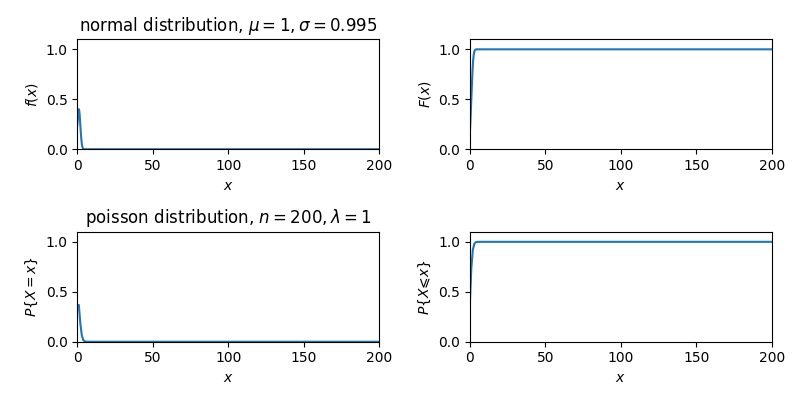
\includegraphics[height=5cm]{5.1.png}
\end{figure}

~

\begin{example}
同上，现设4名维修工，有两个方案，(A) 4名维修工各负责50台设备，(B) 4名维修工分2组，每2名一组，每组负责100台设备，试分析哪个方案较为合理。
\end{example}

解：

每台故障依然如上：
\begin{align*}
&X_i\sim B\left( 1,p \right) \\
&p=\frac{1}{200} \\
&\mu =EX_i=p=\frac{1}{200} \\
&\sigma ^2=DX_i=p\left( 1-p \right) =\frac{199}{200\cdot 200}
\end{align*}

(A) 当每人负责50台设备时，相当于将200台设备分4组，令每组故障数为随机变量$Y_i,i=1,2,3,4$，则有：
\begin{align*}
&Y_i\sim N\left( n\mu ,n\sigma ^2 \right) \overset{n=50}{=}N\left( \frac{50}{200},\frac{50\cdot 199}{200\cdot 200} \right) \\
&P\left\{ Y_i\leqslant y \right\} =\varPhi \left( \frac{y-\mu}{\sigma} \right) =\varPhi \left( \frac{y-\frac{50}{200}}{\sqrt{\frac{50\cdot 199}{200\cdot 200}}} \right) =\varPhi \left( \frac{y-1/4}{\sqrt{199/800}} \right)
\end{align*}
要使设备故障时都能及时得到维修，则
\begin{align*}
P&=P\left\{ Y_1\leqslant 1,Y_2\leqslant 1,Y_3\leqslant 1,Y_4\leqslant 1 \right\} \\
&=P\left\{ Y_1\leqslant 1 \right\} \cdot P\left\{ Y_2\leqslant 1 \right\} \cdot P\left\{ Y_3\leqslant 1 \right\} \cdot P\left\{ Y_4\leqslant 1 \right\} \\
&=\varPhi \left( \frac{1-1/4}{\sqrt{199/800}} \right) ^4=\varPhi \left( 1.5038 \right) ^4=0.9332^4 \\
&=0.758
\end{align*}

(B) 当每2人负责100台设备时，相当于将200台设备分2组，令每组故障数为随机变量$Y_i,i=1,2$，则有：
\begin{align*}
&Y_i\sim N\left( n\mu ,n\sigma ^2 \right) \overset{n=100}{=}N\left( \frac{100}{200},\frac{100\cdot 199}{200\cdot 200} \right) \\
&P\left\{ Y_i\leqslant y \right\} =\varPhi \left( \frac{y-\mu}{\sigma} \right) =\varPhi \left( \frac{y-\frac{100}{200}}{\sqrt{\frac{100\cdot 199}{200\cdot 200}}} \right) =\varPhi \left( \frac{y-1/2}{\sqrt{199/400}} \right)
\end{align*}
要使设备故障时都能及时得到维修，则
\begin{align*}
P&=P\left\{ Y_1\leqslant 2,Y_2\leqslant 2 \right\} \\
&=P\left\{ Y_1\leqslant 2 \right\} \cdot P\left\{ Y_2\leqslant 2 \right\} \\
&=\varPhi \left( \frac{2-1/2}{\sqrt{199/400}} \right) ^2=\varPhi \left( 2.1266 \right) ^2=0.983^2 \\
&=0.966
\end{align*}

可见，方案B故障及时维修的概率更大，更合理。






\newpage
\section{本章小结}

本章简单介绍了大数定理和中心极限定理。

两个定理都是描述独立重复试验。
大数定理阐释了当试验重复次数足够多时，观察值的均值趋于稳定这一现象。
中心极限定理阐释了当试验重复次数足够多时，观察值的和趋于正态分布这一现象。










\chapter{数理统计基础}

前五章我们讨论了概率论，本章开始介绍数理统计。
概率论和数理统计密不可分，前者是后者的理论基础，后者是前者的工程应用。
本章介绍数理统计的基本概念，作为之后章节的基础。

本章要点：
\begin{itemize}
    \item 总体和样本。
    \item 统计量和常见的抽样分布。
\end{itemize}

\newpage
\section{数理统计的基本概念}

本节介绍数理统计的基本概念。

本节要点：
\begin{itemize}
    \item 掌握总体和个体的概念；
    \item 掌握样本和样本值的概念；
    \item 掌握统计量的概念，并熟悉常用的样本的矩；
    \item 掌握上侧分位点的概念。
\end{itemize}

%============================================================
\subsection{总体和样本的概念}

\begin{definition}[总体和个体]
我们将研究问题中的所有被考察对象的全体称为{\bf 总体}，其中的每个成员称为{\bf 个体}。
如果总体包含的个体数量是有限的，则该总体称为{\bf 有限总体}，有限总体的分布总是离散型的，如考试分数。
反之如果个体数量是无限的，则该总体称为{\bf 无限总体}，无限总体的分布可能是离散的、连续的或不定的，如身高。
通常我们考察的是对象的某个量化指标（暂记作$X$），而$X$往往是一个随机变量，所以$X$的分布代表了总体的分布。
因此，我们一般将总体和$X$的分布视作等同，并称为{\bf 总体$X$}。
\end{definition}

例，当我们研究初一学生的身高时，某个学校的所有初一学生可视作总体，每个初一学生即为个体。
我们可以假设身高服从正态分布，于是这个总体的概率分布是正态分布。

例，当我们研究一个批次灯泡的使用寿命时，该批次所有灯泡为总体，每个灯泡为个体。
我们假定使用寿命服从指数分布，于是这个总体的概率分布是指数分布。

很多情况下，总体数量非常大，不可能一一研究，或者像灯泡寿命的例子中，即便灯泡数量不多，我们也不可能测量每个灯泡的使用寿命。
这时，我们需要从总体中选取一些个体进行研究。

\begin{definition}[样本和样本值]
从总体$X$中按一定规则（每个个体抽取机会相等）任意抽取$n$个个体组成的集合$\left( X_1,X_2,\cdots ,X_n \right) $，称为来自总体$X$的一个样本，其中$n$称为样本容量。
若这个规则还满足：
\begin{itemize}
    \item 代表性：即每个个体的指标$X_i$和总体的指标$X$同分布；
    \item 独立性：抽取的个体之间相互独立，
\end{itemize}
这样的样本称为{\bf 简单随机样本}。
抽取后，样本$\left( X_1,X_2,\cdots ,X_n \right) $可视作一个$n$维随机变量，试验后可得到一组确定的数值，称为{\bf 样本值}或{\bf 观察值}，一般记作$\left( x_1,x_2,\cdots x_n \right) $。
\end{definition}

当总体的数量无限多，或者比样本容量大很多的情况下，抽取过程可视为独立。
当总体数量不太多时，抽取过程会对总体的分布有影响，这样的抽取就不能视作独立。

\begin{tcolorbox}
本笔记将样本定义为集合，所以是“一个样本”，有些教材将样本视作集合中的元素，称为“一组样本”，本笔记有时也做类似处理，需结合上下文确定。
\end{tcolorbox}

%============================================================
\subsection{统计量的概念和样本的矩}

\begin{definition}[统计量]
设总体$X$的一个样本$\left( X_1,X_2,\cdots ,X_n \right) $及其样本值$\left( x_1,x_2,\cdots ,x_n \right) $，若有一个$n$元函数
\[
G=g\left( X_1,X_2,\cdots ,X_n \right)
\]
其值不依赖于总体$X$的任何未知参数，就称该$n$元函数为{\bf 该样本的一个统计量}，同时称$g=g\left( x_1,x_2,\cdots ,x_n \right) $为{\bf 统计量的观察值}。
\end{definition}

统计量本质上是一个函数，统计量不能包含总体的任何未知信息，其观察值只取决于样本。
于是我们可以通过选取合适的统计量，计算分析总体的未知信息，如用样本的均值代替总体的数学期望，这就是参数估计。

同时，因为自变量是随机变量，所以统计量也是一个随机变量，有它自己的概率分布。
我们通过样本值计算统计量的观察值，并根据统计量的概率分布判断这次抽样结果是大概率事件还是小概率事件，如果是小概率事件，则说明总体和我们的预期有不同的地方，这就是假设检验。

~

对样本的矩计算是常见统计量，设总体$X$的一个样本$\left( X_1,X_2,\cdots ,X_n \right) $：
\begin{itemize}
    \item {\bf 样本均值}：$\bar{X}=\frac{1}{n}\sum_{i=1}^n{X_i}$
    \item {\bf 样本方差}：$S^2=\frac{1}{n-1}\sum_{i=1}^n{\left( X_i-\bar{X} \right) ^2}=\frac{1}{n-1}\left( \sum_{i=1}^n{{X_i}^2}-n\bar{X}^2 \right) $
    \item {\bf 样本标准差}：$S=\sqrt{S^2}$
    \item {\bf 样本$k$阶原点矩}：$A_k=\frac{1}{n}\sum_{i=1}^n{{X_i}^k}$
    \item {\bf 样本$k$阶中心距}：$B_k=\frac{1}{n}\sum_{i=1}^n{\left( X_i-\bar{X} \right) ^k}$
\end{itemize}

1阶矩有如下关系：
\begin{itemize}
    \item $A_1=\bar{X}$
    \item $A_2={A_1}^2+\frac{n-1}{n}S^2={A_1}^2+B_2$
    \item $B_1=0$
    \item $B_2=\frac{n-1}{n}S^2=A_2-{A_1}^2$
\end{itemize}

~

总体$X$的方差$DX:=E\left[ \left( X-EX \right) ^2 \right] $对应2阶中心距，但样本的方差不对应样本的2阶中心距，两者有一个修正：
\[
B_2=\frac{n-1}{n}S^2
\]
这个修正是为了样本方差能无偏地估计总体方差而设定，所以上述的样本方差也称为{\bf 修正的样本方差}，样本的2阶中心距也称为{\bf 未修正的样本方差}。

由于矩的概念将在后续矩估计法中广泛使用，下面特别将总体的矩和样本的矩做表格对比。

\begin{table}[h]
\centering
\caption{总体和样本的矩}
\begin{tabular}{ccc}
    \toprule
    & 总体 & 样本\\
    \midrule
    $k$阶原点矩 & $E\left[ X^k \right] $ & $A_k=\frac{1}{n}\sum_{i=1}^n{{X_i}^k}$\\
    1阶原点矩 & 总体数学期望$EX$ & 样本均值$A_1=\bar{X}$\\
    2阶原点矩 & & $A_2={A_1}^2+\frac{n-1}{n}S^2$\\
    $k$阶中心矩 & $E\left[ X^k \right] $ & $B_k=\frac{1}{n}\sum_{i=1}^n{\left( X_i-\bar{X} \right) ^k}$\\
    1阶中心矩 & $E\left( X-EX \right) =0$ & $B_1=0$\\
    2阶中心矩 & 总体方差$DX$ & $B_2=\frac{n-1}{n}S^2=A_2-{A_1}^2$\\
    \bottomrule
\end{tabular}
\end{table}

%============================================================
\subsection{上侧分位点的概念}

\begin{definition}[上侧分位点]
设一维随机变量$X$，实数$\alpha \in \left( 0,1 \right) $表示概率，若存在$x_{\alpha}$满足：
\begin{align*}
&P\left\{ X\geqslant x_{\alpha} \right\} \geqslant \alpha \\
&P\left\{ X\leqslant x_{\alpha} \right\} \geqslant 1-\alpha
\end{align*}
则称$x_{\alpha}$为$X$的{\bf 上侧$\alpha $分位点}，或{\bf 右侧$\alpha $分位点}。
\end{definition}

显然，正态分布必有上侧分位点，且唯一，即$\forall \alpha \in \left( 0,1 \right) $，均有唯一的$x_{\alpha}$满足：
\begin{align*}
&P\left\{ X\geqslant x_{\alpha} \right\} =\alpha \\
&P\left\{ X\leqslant x_{\alpha} \right\} =1-\alpha
\end{align*}
而且根据正态分布的对称性有：
\[
x_{1-\alpha}=-x_{\alpha}
\]

\begin{tcolorbox}
上侧$\alpha $分位点常用于区间估计和假设检验。
\end{tcolorbox}

%============================================================
\subsection{例}

\begin{example}
设无限总体有如下分布律
\[
X\sim \left( \begin{matrix}
	0&		1&		2\\
	\frac{1}{6}&		\frac{1}{2}&		\frac{1}{3}\\
\end{matrix} \right)
\]
若抽取4个作为样本，计算至少一个样本值小于等于1的概率。
\end{example}

解：

由于总体无限，所以在抽取过程不会影响总体分布，也即每个样本均服从总体的分布。我们计算所有样本值均为2的概率：
\[
P=P\left\{ X_1=2,X_2=2,X_3=2,X_4=2 \right\}
\]
由于抽取的独立性要求，有：
\begin{align*}
P&=P\left\{ X_1=2 \right\} \cdot P\left\{ X_2=2 \right\} \cdot P\left\{ X_3=2 \right\} \cdot P\left\{ X_4=2 \right\} \\
&=\frac{1}{3}\cdot \frac{1}{3}\cdot \frac{1}{3}\cdot \frac{1}{3}=\frac{1}{81}
\end{align*}
可得，至少一个样本值小于等于1的概率$1-1/18=80/81$。

~

\begin{example}
设总体服从正态分布$X\sim N\left( \mu ,\sigma ^2 \right) $，从总体中抽取一个样本$\left( X_1,X_2,\cdots ,X_n \right) $，若$\mu $已知但$\sigma $未知，分析下列函数能否称为统计量。
\begin{enumerate}
    \item $\bar{X}$
    \item $g\left( X_1,X_2,\cdots ,X_n \right) =\sum_{i=1}^n{\left( X_i-\mu \right)}$
    \item $g\left( X_1,X_2,\cdots ,X_n \right) =\frac{1}{\sigma ^2}\sum_{i=1}^n{\left( X_i-\mu \right)}$
\end{enumerate}
\end{example}

解：

1. $\bar{X}=\frac{\sum{X_i}}{n}$，可见$\bar{X}$不依赖总体的任何参数，是统计量。

2. 函数依赖总体的$\mu $，且$\mu $已知，是统计量。

3. 函数依赖总体的$\mu ,\sigma $，但$\sigma $未知，不是统计量。

~

\begin{example}
设总体服从正态分布$X\sim N\left( \mu ,\sigma ^2 \right) $，从总体抽取一个样本为$\left( X_1,X_2,\cdots ,X_n \right) ,n\geqslant 2$，计算$E\bar{X},D\bar{X},E\left( S^2 \right) $。
\end{example}

解：

抽取具备独立性，所以每个样本有$X_i\sim N\left( \mu ,\sigma ^2 \right) $，于是：
\[
\sum_{i=1}^n{X_i}\sim N\left( n\mu ,n\sigma ^2 \right)
\]
得：
\begin{align*}
&E\bar{X}=E\left( \frac{1}{n}\sum_{i=1}^n{X_i} \right) =\frac{1}{n}\cdot E\left( \sum_{i=1}^n{X_i} \right) =\frac{1}{n}\cdot n\mu \\
&D\bar{X}=D\left( \frac{1}{n}\sum_{i=1}^n{X_i} \right) =\frac{1}{n^2}\cdot D\left( \sum_{i=1}^n{X_i} \right) =\frac{1}{n^2}\cdot n\sigma ^2=\frac{1}{n}\sigma ^2 \\
&\because \begin{cases}
	E\left( \sum{{X_i}^2} \right) =\sum{E\left( {X_i}^2 \right)}=\sum{\left[ DX_i+E\left( X_i \right) ^2 \right]}=n\sigma ^2+n\mu ^2\\
	E\left( n\bar{X}^2 \right) =nE\left( \bar{X}^2 \right) =n\left[ D\bar{X}+E\left( \bar{X} \right) ^2 \right] =\sigma ^2+n\mu ^2\\
\end{cases} \\
&\begin{aligned}
	\therefore E\left( S^2 \right) &=E\left( \frac{\sum{{X_i}^2}-n\bar{X}^2}{n-1} \right) =\frac{1}{n-1}E\left( \sum{{X_i}^2} \right) -\frac{1}{n-1}E\left( n\bar{X}^2 \right)\\
	&=\frac{n\sigma ^2+n\mu ^2-\sigma ^2-n\mu ^2}{n-1}=\sigma ^2\\
\end{aligned}
\end{align*}






\newpage
\section{抽样分布}

本节介绍统计量的概率分布——抽样分布。
总体是决定统计量的因素之一，而总体的分布千千万万，所以这里只讨论基于标准正态分布的总体$X\sim N\left( 0,1 \right) $的样本的统计量。

本节要点：
\begin{itemize}
    \item 掌握抽样分布的概念；
    \item 了解3中常见的分布，卡方分布、t分布、F分布。
\end{itemize}

%============================================================
\subsection{抽样分布的概念}

\begin{definition}[抽样分布]
由于样本具有随机性，所以统计量也具备随机性，我们将统计量的分布称为{\bf 抽样分布}。
\end{definition}

抽样分布在假设检验中发挥重要作用。
统计量本质上是一个函数，其值的分布带有随机特征，所以通过统计量的观察值就可以判断该次抽取样本的试验是小概率事件还是大概率事件，如果是小概率事件，则可能表示总体发生了些变化。

%============================================================
\subsection{卡方分布}

\begin{definition}[卡方分布]
设总体$X\sim N\left( 0,1 \right) $的一个样本$\left( X_1,X_2,\cdots ,X_n \right) $，记它们的平方和的统计量为$\chi ^2$，称$\chi ^2$的分布为{\bf 服从自由度为$n$的$\chi ^2$分布}，记作$\chi ^2\sim \chi ^2\left( n \right) $，即：
\[
\chi ^2:=\sum_{i=1}^n{{X_i}^2}
\]
\end{definition}

\begin{tcolorbox}
注意，记号$\chi ^2\sim \chi ^2\left( n \right) $中，第一个$\chi ^2$表示统计量，第二个$\chi ^2$表示分布。
\end{tcolorbox}

$\chi ^2$的密度函数为：
\[
f\left( x,n \right) =\begin{cases}
	0&		x\leqslant 0\\
	\frac{1}{2^{\frac{n}{2}}\varGamma \left( \frac{n}{2} \right)}x^{\frac{n}{2}-1}e^{-\frac{x}{2}}&		x>0\\
\end{cases}
\]
其中：
\begin{itemize}
    \item $x=\sum_{i=1}^n{{x_i}^2}$：统计量的观察值，即样本值的平方和；
    \item $n$：自由度，决定了函数的形状；
    \item $\varGamma \left( p \right) =\int_0^{+\infty}{x^{p-1}e^{-x}dx},p>0$：称为{\bf $\varGamma $函数}。
\end{itemize}
以自由度为1，3，5，10为例，密度函数的图形如下：

\begin{figure}[h]
\centering
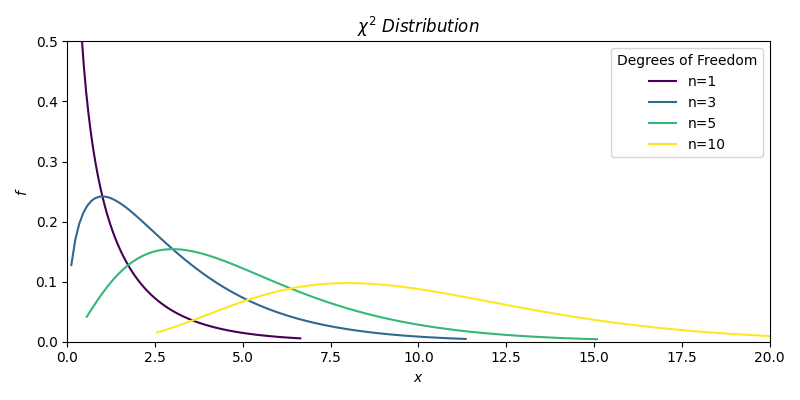
\includegraphics[height=5cm]{6.1.png}
\end{figure}

卡方分布$\chi ^2\sim \chi ^2\left( n \right) $的性质：
\begin{itemize}
    \item 有期望和方差$E\left( \chi ^2 \right) =n,D\left( \chi ^2 \right) =2n$；
    \item 当自由度$n\rightarrow +\infty $时，卡方分布近似为正态分布$\chi ^2\sim N\left( n,2n \right) $；
    \item 总体$X\sim N\left( 0,1 \right) $自己的平方和服从自由度为1的卡方分布$X\sim \chi ^2\left( 1 \right) $；
    \item 设$k$个服从卡方分布的随机变量$\chi _{i}^{2}\sim \chi ^2\left( n_i \right) ,i=1,2,\cdots ,k$，且各个$\chi _{i}^{2}$相互独立，则它们的和依然服从卡方分布，且自由度为各自自由度的和，称为{\bf 卡方分布的可加性}，即：
	\[
	\sum_{i=1}^k{\chi _{i}^{2}}\sim \chi ^2\left( \sum_{i=1}^k{n_i} \right)
	\]
    \item 卡方分布有唯一的上侧$\alpha $分位点，一般记作$\chi _{\alpha}^{2}\left( n \right) $，当自由度$n\rightarrow +\infty $时，$\chi _{\alpha}^{2}\left( n \right) \rightarrow n+\sqrt{2n}u_{\alpha},\chi _{1-\alpha}^{2}\left( n \right) \rightarrow n-\sqrt{2n}u_{\alpha}$，其中$u_{\alpha}$为标准正态分布的上侧$\alpha $分位点。
\end{itemize}

\begin{tcolorbox}
卡方分布由Karl Pearson于1900年提出，用于衡量观测值与理论值之间的差异。
从表达式看，卡方分布的物理意义是物体的转动惯量，但和方差不同，卡方分布没有减取均值，所以它带有质量分布和质量中心位置两个信息。
当我们假设总体分布为标准正态分布时，抽样得到的卡方值大概率会集中于一个范围，若卡方值出现在小概率地方，则说明我们的假设很可能不对。
\end{tcolorbox}

%============================================================
\subsection{t分布}

\begin{definition}[t分布]
设两个相互独立的随机变量$X\sim N\left( 0,1 \right) ,Y\sim \chi ^2\left( n \right) $，记如下的统计量为$T$，称$T$的分布为{\bf 服从自由度为$n$的$t$分布}，记作$T\sim t\left( n \right) $：
\[
T:=\frac{X}{\sqrt{Y/n}}
\]
\end{definition}

$T$的密度函数为：
\[
f\left( x,n \right) =\frac{\varGamma \left( \frac{n+1}{2} \right)}{\sqrt{n\pi}\varGamma \left( \frac{n}{2} \right)}\left( 1+\frac{x^2}{n} \right) ^{-\frac{n+1}{2}}, \qquad x\in \mathbb{R}
\]

以自由度为1，3，5，1000为例，密度函数图形如下：
\begin{figure}[h]
\centering
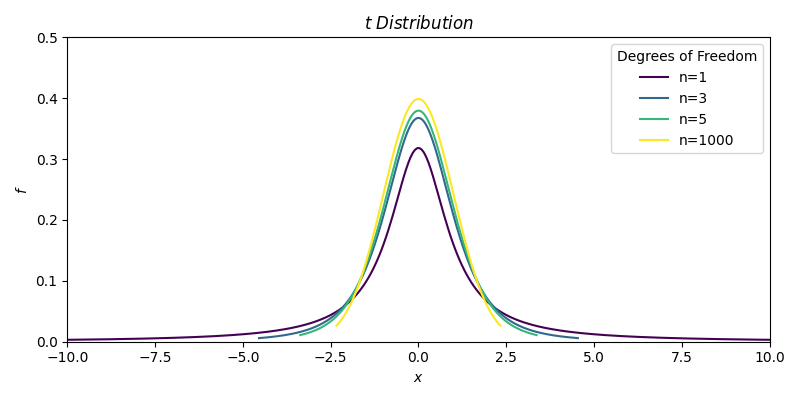
\includegraphics[height=5cm]{6.2.png}
\end{figure}

$T\sim t\left( n \right) $分布的性质：
\begin{itemize}
    \item 有期望和方差$ET=0\quad n>1,\quad DT=\frac{n}{n-2}\quad n>2$；
    \item 当自由度$n\rightarrow +\infty $时，$T$分布近似为标准正态分布$T\sim N\left( 0,1 \right) $；
    \item $T$分布有唯一的上侧$\alpha $分位点，一般记作$t_{\alpha}\left( n \right) $，且根据对称性有$t_{1-\alpha}\left( n \right) =-t_{\alpha}\left( n \right) $，当自由度$n\rightarrow +\infty $时，$t_{\alpha}\left( n \right) \rightarrow u_{\alpha}$，其中$u_{\alpha}$为标准正态分布的上侧$\alpha $分位点。
\end{itemize}

\begin{tcolorbox}
t分布由William Sealy Gosset在1908年提出。
从表达式看，t分布是用样本对标准正态分布的一种修正，在没有充足样本时，给出一个“更保守的正态分布”，常用于区间估计。
\end{tcolorbox}

%============================================================
\subsection{F分布}

\begin{definition}[F分布]
设两个相互独立的随机变量$X\sim \chi ^2\left( n_1 \right) ,Y\sim \chi ^2\left( n_2 \right) $，记如下的统计量为$F$，称$F$的分布为{\bf 服从第一自由度为$n_1$第二自由度为$n_2$的$F$分布}，记作$F\sim F\left( n_1,n_2 \right) $：
\[
F:=\frac{X/n_1}{Y/n_2}
\]
\end{definition}

\begin{tcolorbox}
记号$F\sim F\left( n_1,n_2 \right) $中，第一个$F$表示统计量，是一个随机变量，第二个$F$表示分布。
\end{tcolorbox}

$F$的密度函数为：
\[
f\left( x,n_1,n_2 \right) =\begin{cases}
	0&		x\leqslant 0\\
	\frac{\varGamma \left( \frac{n_1+n_2}{2} \right)}{\varGamma \left( \frac{n_1}{2} \right) \varGamma \left( \frac{n_2}{2} \right)}{n_1}^{\frac{n_1}{2}}{n_2}^{\frac{n_2}{2}}x^{\frac{n_1}{2}-1}\left( n_1x+n_2 \right) ^{-\frac{n_1+n_2}{2}}&		x>0\\
\end{cases}
\]

以自由度为3，5，10，20为例，密度函数图形如下：
\begin{figure}[h]
\centering
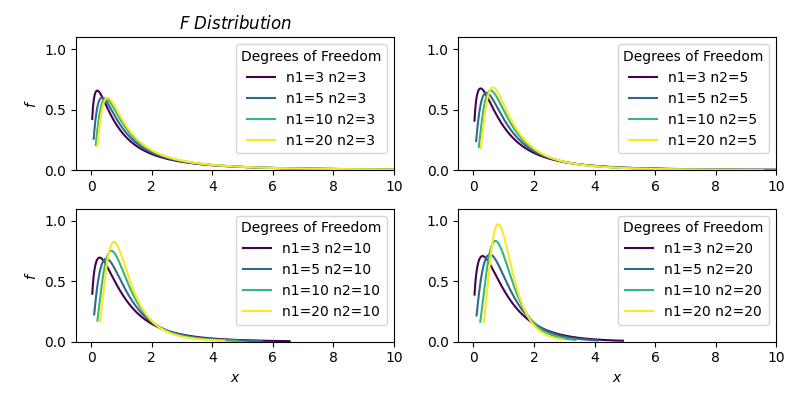
\includegraphics[height=5cm]{6.3.png}
\end{figure}

$F\sim F\left( n_1,n_2 \right) $分布的性质：
\begin{itemize}
    \item 有期望和方差$EF=\frac{n_2}{n_2-2}\quad n_2>1,\quad DF=\frac{2{n_2}^2\left( n_1+n_2-2 \right)}{n_1\left( n_2-2 \right) ^2\left( n_2-4 \right)}\quad n_2>4$；
    \item 若有随机变量$T\sim t\left( n \right) $，则$T^2\sim F\left( 1,n \right) $；
    \item 若有随机变量$F\sim F\left( n_1,n_2 \right) $，则$\frac{1}{F}\sim F\left( n_2,n_1 \right) $；
    \item $F$分布有唯一的上侧$\alpha $分位点，一般记作$F_{\alpha}\left( n_1,n_2 \right) $，且有
	
	$F_{1-\alpha}\left( n_1,n_2 \right) =\frac{1}{F_{\alpha}\left( n_1,n_2 \right)}$。
\end{itemize}

\begin{tcolorbox}
F分布由英国统计学家Ronald.A.Fisher在20世纪20年代提出。
从表达式看，F分布比较两个样本的方差，以判断整体均值是否存在显著差异。
\end{tcolorbox}

%============================================================
\subsection{正态总体的样本的抽样分布}

以上讨论的是总体$X\sim N\left( 0,1 \right) $的样本的抽样分布，下面扩展到正态分布的总体。

\begin{theorem}
设有服从正态分布的总体$X\sim N\left( \mu ,\sigma ^2 \right) $，$\left( X_1,X_2,\cdots ,X_n \right) $为其一样本，则：
\begin{itemize}
    \item 样本均值$\bar{X}$服从正态分布，$\bar{X}\sim N\left( \mu ,\frac{\sigma ^2}{n} \right) $或$\frac{\bar{X}-\mu}{\sqrt{\sigma ^2/n}}\sim N\left( 0,1 \right) $；
    \item $\frac{\sum_{i=1}^n{\left( X_i-\mu \right) ^2}}{\sigma ^2}\sim \chi ^2\left( n \right) $，用于$\mu ,\sigma $已知的情况；
    \item $\frac{\sum_{i=1}^n{\left( X_i-\bar{X} \right) ^2}}{\sigma ^2}\sim \chi ^2\left( n-1 \right) $，且$\bar{X},S^2$相互独立，用于$\sigma $已知$\mu $未知的情况，用$\bar{X}$代替$\mu $；
    \item $\frac{\bar{X}-\mu}{S/\sqrt{n}}\sim t\left( n-1 \right) $，用于$\mu $已知$\sigma $未知的情况，用$S$代替$\sigma $。
\end{itemize}
\end{theorem}

\begin{tcolorbox}
对于两个正态分布的总体的讨论，见“教材\cite{book1}”，P193。
\end{tcolorbox}






\newpage
\section{本章小结}

本章作为数理统计的基础，介绍了几个基本概念和3种常见的分布。

~

{\bf 总体}和{\bf 样本}

总体是所有考察对象的集合，这种“所有”往往带有不可穷尽，所以实际中我们通过获取部分对象，即样本$\left( X_1,X_2,\cdots ,X_n \right) $，考察总体的性质。
样本是一个$n$维随机变量。

{\bf 统计量}和{\bf 抽样分布}

统计量$g\left( X_1,X_2,\cdots ,X_n \right) $是样本的函数，一个多元随机变量函数，其值是必须能通过样本完全确定，才能用来估计总体。
其次，统计量也是一个随机变量，有自己的分布，称为抽样分布，具体形态由总体、统计量的函数形式$g$、样本的容量$n$共同决定。
好的抽样分布能反映总体的情况，常见的有卡方分布、t分布、F分布。










\chapter{参数估计}

本章讨论参数估计及其评价方法。
参数估计是数理统计的一个基本问题，讨论的是如何使用样本估计总体的未知信息。

参数估计有点估计和区间估计：
\begin{itemize}
    \item 点估计：用样本估计总体的分布的未知参数，有矩估计法、极大似然估计法、贝叶斯估计法等；
    \item 区间估计：估计未知参数的取值范围。
\end{itemize}

本章要点：
\begin{itemize}
    \item 矩估计法。
    \item 极大似然估计法。
    \item 估计量的评价标准。
    \item 区间估计。
\end{itemize}

\newpage
\section{点估计}

本节介绍点估计，点估计是用样本推断总体的一大类方法，本节介绍两种点估计方法——矩估计法和极大似然估计法。

本节要点：
\begin{itemize}
    \item 了解点估计的应用意义；
    \item 深刻理解矩估计法，并熟练掌握；
    \item 深刻理解极大似然估计法，并熟练掌握。
\end{itemize}

%============================================================
\subsection{点估计的基础概念}

在实际应用中，可能知道某个总体的分布类型，但不知道具体形式。
如知道元件寿命服从指数分布，但不知道失效率$\lambda $的具体值。
对此，我们可以抽取一个样本并测试得到观察值$\left( x_1,x_2,\cdots x_n \right) $，用该观察值估计$\lambda $。

一般地讲，若总体$X$的分布含有$k$个未知参数，这些未知参数可一并记作一个向量$\boldsymbol{\theta }=\left( \theta _1,\theta _2,\cdots ,\theta _k \right) $，此时，总体的密度函数可以记作：
\[
f\left( x;\boldsymbol{\theta } \right)
\]
设有样本$\left( X_1,X_2,\cdots ,X_n \right) $，则可以根据样本的若干个统计量去估计$\boldsymbol{\theta }$，该这些统计量称为{\bf 估计量}，记作$\hat{\theta}$，一般$k$个未知参数需要$k$个估计量，即：
\begin{align*}
&\hat{\theta}_1\left( X_1,X_2,\cdots ,X_n \right) \\
&\hat{\theta}_2\left( X_1,X_2,\cdots ,X_n \right) \\
&\cdots \\
&\hat{\theta}_k\left( X_1,X_2,\cdots ,X_n \right)
\end{align*}
当样本的观察值为$\left( x_1,x_2,\cdots ,x_n \right) $时，称$\hat{\theta}\left( x_1,x_2,\cdots ,x_n \right) $为{\bf 估计值}。

点估计的本质就是用样本观察值推断总体的分布，最简单的估计值是样本的均值，只要样本容量够大，我们就可以将样本均值当作总体的期望。

%============================================================
\subsection{矩估计法的概念}

矩估计法由英国统计学家K.皮尔逊在19世纪末到20世纪初的一系列文章中提出，其核心思想是{\bf 用样本的矩替代总体的矩}。
如，若总体含有2个未知参数，则总体期望对应样本均值，总体方差对应样本2阶中心距：
\begin{align*}
&EX\leftrightarrow A_1=\bar{X}=\frac{1}{n}\sum_{i=1}^n{X_i} \\
&DX\leftrightarrow B_2=\frac{n-1}{n}S^2=A_2-{A_1}^2
\end{align*}
实际使用中，我们通常用样本方差代替总体方差。
由大数定理可知，当样本容量足够大时，上述对应关系可视作相等：
\begin{align*}
&EX\leftrightarrow A_1=\bar{X}=\frac{1}{n}\sum_{i=1}^n{X_i} \\
&DX\leftrightarrow S^2=\frac{n}{n-1}B_2=\frac{1}{n-1}\left( \sum_{i=1}^n{{X_i}^2}-n\bar{X}^2 \right)
\end{align*}
若总体含有3个及以上个未知参数，则使用高阶矩。

\begin{tcolorbox}
$DX$的估计量的表达式不唯一，所以估计值也并不唯一。
\end{tcolorbox}

\begin{definition}[矩估计法]
设有总体$X$及其一个样本$\left( X_1,X_2,\cdots ,X_n \right) $，将以样本的$k$阶原点矩$A_k=\frac{1}{n}\sum_{i=1}^n{{X_i}^k}$作为总体的$k$阶原点矩所计算得到的总体的参数的方法称为{\bf 矩估计法}，由该方法得到的估计量称为{\bf 矩估计量}，将样本观察值带入后得到的数值称为{\bf 矩估计值}。
\end{definition}

%============================================================
\subsection{矩估计法的用法}

矩估计法按照低矩优先的原则进行计算。
一般地，若总体$X$只涉及一个未知参数，如指数分布$X\sim E\left( \lambda \right) $，则根据指数分布的期望，只需要使用1阶原点矩即可得到：
\begin{align*}
&\because \begin{cases}
	EX=\frac{1}{\lambda}\\
	EX\leftrightarrow A_1=\bar{X}=\frac{1}{n}\sum_{i=1}^n{X_i}\\
\end{cases} \\
&\therefore \lambda \leftrightarrow \hat{\lambda}=\frac{1}{\bar{X}}
\end{align*}
若总体$X$涉及两个未知参数，如正态分布$X\sim N\left( \mu ,\sigma ^2 \right) $，则需要计算2阶矩：
\begin{align*}
&\because \begin{cases}
	EX=\mu\\
	DX=\sigma ^2\\
	EX\leftrightarrow A_1=\bar{X}=\frac{1}{n}\sum_{i=1}^n{X_i}\\
	DX\leftrightarrow S^2=\frac{1}{n-1}\left( \sum_{i=1}^n{{X_i}^2}-n\bar{X}^2 \right)\\
\end{cases} \\
&\therefore \begin{cases}
	\mu \leftrightarrow \hat{\mu}=\bar{X}\\
	\sigma ^2\leftrightarrow \hat{\sigma}^2=S^2\\
\end{cases}
\end{align*}

%============================================================
\subsection{例}

\begin{example}
设总体$X$的密度函数
\[
f\left( x;\theta \right) =\begin{cases}
	e^{-\left( x-\theta \right)}&		x\geqslant \theta\\
	0&		x<\theta\\
\end{cases}
\]
其中$\theta $未知，分析如何大致确定该密度函数。
\end{example}

解：

只有1个未知参数，按照低矩优先原则，使用1阶原点矩。首先分析总体的期望：
\[
EX=\int_{-\infty}^{+\infty}{xf\left( x \right) \cdot dx}=\int_0^{+\infty}{xe^{-\left( x-\theta \right)}\cdot dx}=1+\theta
\]
若要确定密度函数，即确定$\theta $对应的估计量$\hat{\theta}$，可获取一个样本，记作$\left( X_1,X_2,\cdots ,X_n \right) $，并计算均值$\bar{X}$，根据矩估计法：
\begin{align*}
&\because EX=1+\theta \leftrightarrow \bar{X} \\
&\therefore 1+\hat{\theta}=\bar{X} \\
&\therefore \hat{\theta}=\bar{X}-1
\end{align*}

~

\begin{example}
设总体$X$有分布律
\[
X\sim \left( \begin{matrix}
	0&		1&		2&		3\\
	\theta ^2&		2\theta \left( 1-\theta \right)&		\theta ^2&		1-2\theta\\
\end{matrix} \right)
\]
$\theta $未知，若获取一个样本为$\left( 3,1,3,0,3,1,2,3 \right) $，试估计$X$的分布律。
\end{example}

解：

只有1个未知参数，按照低矩优先原则，使用1阶原点矩。首先分析总体的期望：
\[
EX=0\cdot \theta ^2+1\cdot 2\theta \left( 1-\theta \right) +2\cdot \theta ^2+3\cdot \left( 1-2\theta \right) =2\theta +3-4\theta
\]
再分析样本的均值：
\[
\bar{X}=\frac{3+1+3+0+3+1+2+3}{8}=2
\]
可得：
\[
3-4\hat{\theta}=2\qquad \Rightarrow \qquad \hat{\theta}=\frac{1}{4}
\]
最终得到总体$X$的分布率大致为：
\[
X\sim \left( \begin{matrix}
	0&		1&		2&		3\\
	\frac{1}{8}&		\frac{3}{8}&		\frac{1}{8}&		\frac{4}{8}\\
\end{matrix} \right)
\]

\begin{tcolorbox}
此例说明，根据样本计算的估计值并不是总体的参数，$\theta \ne \hat{\theta}$，按照$\hat{\theta}$得到的总体分布会有误差。
\end{tcolorbox}

~

\begin{example}
设总体$X$有分布律
\[
X\sim \left( \begin{matrix}
	0&		1&		2&		3\\
	{\theta _1}^2&		2\left( \theta _2-{\theta _1}^2 \right)&		{\theta _1}^2&		1-2\theta _2\\
\end{matrix} \right)
\]
$\theta _1,\theta _2$未知，若获取一个样本为$\left( 3,1,3,0,3,1,2,3 \right) $，试估计$X$的分布律。
\end{example}

解：

只有2个未知参数，按照低矩优先原则，使用1阶原点矩和2阶原点矩。
首先分析总体的期望和2阶原点矩：
\begin{align*}
EX&=0\cdot {\theta _1}^2+1\cdot 2\left( \theta _2-{\theta _1}^2 \right) +2\cdot {\theta _1}^2+3\cdot \left( 1-2\theta _2 \right) \\
&=3-4\theta _2 \\
E\left( X^2 \right) &=0\cdot {\theta _1}^2+1^2\cdot 2\left( \theta _2-{\theta _1}^2 \right) +2^2\cdot {\theta _1}^2+3^2\cdot \left( 1-2\theta _2 \right) \\
&=2{\theta _1}^2+9-16\theta _2
\end{align*}
再分析样本的均值和2阶原点矩：
\begin{align*}
&\bar{X}=\frac{3+1+3+0+3+1+2+3}{8}=2 \\
&A_2=\frac{3^2+1^2+3^2+0^2+3^2+1^2+2^2+3^2}{8}=\frac{42}{8}
\end{align*}
可得：
\[
\begin{cases}
	3-4\hat{\theta}_2=\bar{X}=2\\
	2{\hat{\theta}_1}^2+9-16\hat{\theta}_2=\frac{42}{8}\\
\end{cases}\quad \Rightarrow \quad \begin{cases}
	\hat{\theta}_2=\frac{1}{4}\\
	\hat{\theta}_1=\sqrt{\frac{1}{8}}=\frac{1}{2\sqrt{2}}\\
\end{cases}
\]
最终得到总体$X$的分布率大致为：
\[
X\sim \left( \begin{matrix}
    0&		1&		2&		3\\
    \frac{1}{8}&		\frac{2}{8}&		\frac{1}{8}&		\frac{4}{8}\\
\end{matrix} \right)
\]

%============================================================
\subsection{极大似然估计法的概念}

极大似然估计法由英国统计学家R.A.费希尔于1912年提出，并在1921年完善。
其核心思想是{\bf 当一个样本的观察值已经发生，总体的未知参数总是倾向于该观察值的概率最大，因为观察值已经发生了}。

具体说明。
设总体$X$的未知参数构成向量$\boldsymbol{\theta }\left( \theta _1,\theta _2,\cdots ,\theta _k \right) $，设抽样得到一样本$\left( X_1,X_2,\cdots ,X_n \right) $的观察值$\left( x_1,x_2,\cdots ,x_n \right) $，由于样本的定义中规定了抽取必须相互独立，所以观察值$\left( x_1,x_2,\cdots ,x_n \right) $发生的概率为各个值的概率的乘积：
\[
P=P_1P_2\cdots P_n=f\left( x_1;\boldsymbol{\theta } \right) \cdot f\left( x_2;\boldsymbol{\theta } \right) \cdot \cdots \cdot f\left( x_n;\boldsymbol{\theta } \right)
\]
$P$应该是最大的。
该方法就是确定$\boldsymbol{\theta }\left( \theta _1,\theta _2,\cdots ,\theta _k \right) $取什么值时，$P$最大。

\begin{definition}[似然函数]
设总体$X$的未知参数构成向量$\boldsymbol{\theta }\left( \theta _1,\theta _2,\cdots ,\theta _k \right) $，设抽取得到一样本$\left( X_1,X_2,\cdots ,X_n \right) $的观察值为$\left( x_1,x_2,\cdots ,x_n \right) $，若将$\boldsymbol{\theta }$视作变量，于是可以构造函数：
\begin{align*}
&L\left( x_1,x_2,\cdots ,x_n;\boldsymbol{\theta } \right) =\prod_{i=1}^n{p\left( x_i;\boldsymbol{\theta } \right)} \\
&L\left( x_1,x_2,\cdots ,x_n;\boldsymbol{\theta } \right) =\prod_{i=1}^n{f\left( x_i;\boldsymbol{\theta } \right)}
\end{align*}
其中：
\begin{itemize}
    \item $p\left( x_i;\boldsymbol{\theta } \right) $：总体为离散随机变量时的分布律；
    \item $f\left( x_i;\boldsymbol{\theta } \right) $：总体为连续随机变量时的密度函数。
\end{itemize}
则称上述函数为{\bf 似然函数}，可简记作$L\left( \boldsymbol{\theta } \right) $。
若当$\boldsymbol{\theta }=\boldsymbol{\hat{\theta}}$时$L$取得最大值，则称$\boldsymbol{\hat{\theta}}$为{\bf 极大似然估计值}。
\end{definition}

\begin{tcolorbox}
所谓的似然函数就是观察值发生的概率。
\end{tcolorbox}

\begin{definition}[极大似然估计法]
设有总体$X$，取一个样本并得到对应的一个样本的观察值$\left( x_1,x_2,\cdots ,x_n \right) $，构造对应的似然函数$L\left( \boldsymbol{\theta } \right) $，将似然函数的极大值点作为总体未知参数的方法，称为{\bf 极大似然估计法}。
\end{definition}

%============================================================
\subsection{极大似然估计法的用法}

可见，极大似然估计法在于求解似然函数的极大值。
求解方法可以使用微积分中的极值求解方法（判断驻点+边界点），由于似然函数是累积函数，求导较为复杂，所以可求解其对数形式的导数，令：
\begin{align*}
&\ln L\left( x_1,x_2,\cdots ,x_n;\boldsymbol{\theta } \right) =\sum_{i=1}^n{p\left( x_i;\boldsymbol{\theta } \right)} \\
&\ln L\left( x_1,x_2,\cdots ,x_n;\boldsymbol{\theta } \right) =\sum_{i=1}^n{f\left( x_i;\boldsymbol{\theta } \right)}
\end{align*}
于是求解方程组：
\begin{align*}
&\frac{\partial}{\partial \boldsymbol{\theta }}\ln L\left( x_1,x_2,\cdots ,x_n;\boldsymbol{\theta } \right) =\sum_{i=1}^n{\frac{\partial p\left( x_i;\boldsymbol{\theta } \right)}{\partial \boldsymbol{\theta }}}=\mathbf{0} \\
&\frac{\partial}{\partial \boldsymbol{\theta }}\ln L\left( x_1,x_2,\cdots ,x_n;\boldsymbol{\theta } \right) =\sum_{i=1}^n{\frac{\partial f\left( x_i;\boldsymbol{\theta } \right)}{\partial \boldsymbol{\theta }}}=\mathbf{0}
\end{align*}
最终得到极大似然估计值$\boldsymbol{\hat{\theta}}$。

%============================================================
\subsection{例}

\begin{example}
设总体$X$的密度函数
\[
f\left( x;\theta \right) =\begin{cases}
    e^{-\left( x-\theta \right)}&		x\geqslant \theta\\
    0&		x<\theta\\
\end{cases}
\]
其中$\theta $未知，用极大似然估计法分析该密度函数。
\end{example}

解：

设取一个样本的样本值为$\left( x_1,x_2,\cdots ,x_n \right) $，构造似然函数：
\begin{align*}
&L\left( x_1,x_2,\cdots ,x_n;\theta \right) =\prod_{i=1}^n{f\left( x_i;\theta \right)}=e^{n\theta -\sum_{i=1}^n{x_i}} \\
&\ln L\left( x_1,x_2,\cdots ,x_n;\theta \right) =n\theta -\sum_{i=1}^n{x_i} \\
&\frac{\partial}{\partial \theta}\ln L\left( x_1,x_2,\cdots ,x_n;\theta \right) =n>0
\end{align*}
为严格单调递增函数，所以$\theta $在取值范围内$\theta \leqslant x_i$取到最大值时为估计值，即$\hat{\theta}=\min \left\{ x_1,x_2,\cdots ,x_n \right\} $。

~

\begin{example}
设总体$X$的分布律
\[
X\sim \left( \begin{matrix}
    0&		1&		2&		3\\
    \theta ^2&		2\theta \left( 1-\theta \right)&		\theta ^2&		1-2\theta\\
\end{matrix} \right)
\]
其中$\theta $未知，若获取一个样本为$\left( 3,1,3,0,3,1,2,3 \right) $，试用极大似然估计法估计$X$的分布律。
\end{example}

解：

构造似然函数：
\begin{align*}
&L\left( x_1,x_2,\cdots ,x_n;\theta \right) =\prod_{i=1}^n{p\left( x_i;\theta \right)} \\
&=\left( 1-2\theta \right) \cdot 2\theta \left( 1-\theta \right) \cdot \left( 1-2\theta \right) \cdot \theta ^2\cdot \left( 1-2\theta \right) \cdot 2\theta \left( 1-\theta \right) \cdot \theta ^2\cdot \left( 1-2\theta \right) \\
&=\left( 1-2\theta \right) ^4\cdot 4\cdot \theta ^6\cdot \left( 1-\theta \right) ^2
\end{align*}
两边取对数求导得估计值$\hat{\theta}$：
\begin{align*}
&\ln L\left( \theta \right) =4\ln \left( 1-2\theta \right) +6\ln \theta +2\ln \left( 1-\theta \right) +\ln 4 \\
&\frac{d}{d\theta}\ln L\left( \theta \right) =-\frac{8}{1-2\theta}+\frac{6}{\theta}-\frac{2}{1-\theta}=0 \\
&\hat{\theta}=\frac{7\pm \sqrt{13}}{12}
\end{align*}
但需注意，作为分布律必须不能小于0，当$\hat{\theta}=\frac{7+\sqrt{13}}{12}$时，$1-2\cdot \hat{\theta}=-0.77$，舍弃，得估计值：
\[
\hat{\theta}=\frac{7-\sqrt{13}}{12}=0.283
\]
最终得到总体$X$的分布率大致为：
\[
X\sim \left( \begin{matrix}
	0&		1&		2&		3\\
	0.08&		0.41&		0.08&		0.43\\
\end{matrix} \right)
\]

\begin{tcolorbox}
对比矩估计法的结果，两个方法在一般情况下得到的估计值不会相同，事实上，不同的估计方法各有优劣。
\end{tcolorbox}

~

\begin{example}
设箱子内白球和黑球4共有个，若采用放回抽样，抽取3次，得到2次白球和1次黑球，分析箱子内有几个白球。
\end{example}

解：

由于是放回抽样，抽到白球服从二项分布：
\[
P\left\{ X=x \right\} =C_{n}^{x}p^x\left( 1-p \right) ^{n-x},\qquad \begin{array}{l}
	x=0,1,\cdots ,n\\
	p\in \left( 0,1 \right)\\
\end{array}
\]
设白球有$\theta $个，由题意可知$n=3,x=2,p=\frac{\theta}{4}$，于是：
\[
P\left\{ X=2 \right\} =C_{3}^{2}\left( \frac{\theta}{4} \right) ^2\left( 1-\frac{\theta}{4} \right) ^1
\]
构造似然函数求极值：
\begin{align*}
&L\left( x;\theta \right) =P\left\{ X=2 \right\} =C_{3}^{2}\left( \frac{\theta}{4} \right) ^2\left( 1-\frac{\theta}{4} \right) ^1=\frac{3}{16}\theta ^2-\frac{3}{64}\theta ^3 \\
&\frac{d}{d\theta}L\left( x;\theta \right) =\frac{3}{8}\theta -\frac{9}{64}\theta ^2=0 \\
&\theta =0\mathrm{or}2.67
\end{align*}
白球应该有3个。






\newpage
\section{估计量的评价标准}

\begin{tcolorbox}
从前一小节可以看出，不同的点估计方法得到的结果不同，所以有必要建立一套评价体系评价每个方法的优劣。
值得注意的是，同一个点估计方法在不同的指标下有不同的优劣，可能在某个指标有优势，但在另一个指标有劣势，而且样本的选取及其不同的观察值对评价结果也有影响，所以在实际应用中，需要根据实际情况判断估计方法的优劣性。
\end{tcolorbox}

本节简单介绍评价点估计方法的指标。

本节要点：
\begin{itemize}
    \item 了解常用的三大评价指标。
\end{itemize}

%============================================================
\subsection{均方误差的概念}

\begin{definition}[均方误差]
设$\hat{\theta}$为$\theta $的估计量，$\hat{\theta}$由样本$\left( X_1,X_2,\cdots ,X_n \right) $确定，也是随机变量，若$E\left[ \left( \hat{\theta}-\theta \right) ^2 \right] $存在，则称之为{\bf 用$\hat{\theta}$估计$\theta $时产生的均方误差}，记作$MSE\left( \hat{\theta} \right) $，即：
\[
MSE\left( \hat{\theta} \right) :=E\left[ \left( \hat{\theta}-\theta \right) ^2 \right]
\]
且有：
\[
MSE\left( \hat{\theta} \right) =D\hat{\theta}+\left( E\hat{\theta}-\theta \right) ^2
\]
\end{definition}

证明略，可见“教材\cite{book1}”。
均方误差的意义在于，$MSE\left( \hat{\theta} \right) $越小，则$\hat{\theta}$受样本不确定性越小。

%============================================================
\subsection{无偏性的概念}

\begin{definition}[无偏性]
设$\hat{\theta}$为$\theta $的估计量，若对于$\theta \in \varTheta $，均有$E\hat{\theta}=\theta $，其中$\varTheta $为$\theta $的取值范围，则称$\hat{\theta}$为$\theta $的{\bf 无偏估计}，反之称为{\bf 有偏估计}。
当$\hat{\theta}$为有偏估计时，若$\underset{n\rightarrow \infty}{\lim}E\hat{\theta}=\theta $，则称$\hat{\theta}$为 的{\bf 渐进无偏估计}。
\end{definition}

无偏性描述了“这个估计量是瞄着总本参数去的”。
如果一个估计量是无偏的，说明该估计量没有系统性偏差，其本身来讲是没有问题的，它的随机性是由样本抽取时的不确定带来的。
如果有偏，则表示无论怎么抽样，估计量总与总体参数存在一定距离。

\begin{theorem}
设总体$X$有期望$EX$和方差$DX$，$\left( X_1,X_2,\cdots ,X_n \right) $为其一样本，则：
\begin{itemize}
    \item $\bar{X}$为$EX$的无偏估计，即$E\bar{X}=EX$；
    \item $S^2$为$DX$的无偏估计，即$E\left( S^2 \right) =DX$。
\end{itemize}
\end{theorem}

证明略，可见“教材\cite{book1}”。
该定理也说明，一般我们使用样本方差$S^2$作为总体方差的估计量，而非样本的2阶中心距。

%============================================================
\subsection{有效性的概念}

\begin{definition}[有效性]
设$\hat{\theta}_1,\hat{\theta}_2,\cdots ,\hat{\theta}_n$均为$\theta $的无偏估计，则$MSE\left( \hat{\theta} \right) =D\hat{\theta}$，若有$D\hat{\theta}_1<D\hat{\theta}_2$，则称{\bf $\hat{\theta}_1$比$\hat{\theta}_2$更有效}。
若存在$\hat{\theta}_k$，它的方差小于任何其他估计量，即$D\hat{\theta}_k\leqslant D\hat{\theta}_i$，则称$\hat{\theta}_k$为$\theta $的{\bf 一致最小方差的无偏估计}。
无偏估计的最小方差不可能无限小，有一个下限，称为{\bf 方差下界}，若某个无偏估计的方差达到该下界，则称之为{\bf 有效估计}。
\end{definition}

有效性描述了由于样本抽取的不确定造成的估计量的误差的离散型。
若一个估计量更有效，说明在同样的抽取规则下，它的随机性越小。

\begin{tcolorbox}
关于方差下界，可阅读“教材\cite{book1}”P216～217和“教材\cite{book2}”P167～170。
\end{tcolorbox}

%============================================================
\subsection{相合性的概念}

\begin{definition}[相合性]
设$\hat{\theta}$为$\theta $的估计量，若对于$\forall \varepsilon $，均有
\[
\underset{n\rightarrow \infty}{\lim}P\left\{ \left| \hat{\theta}-\theta \right|<\varepsilon \right\} =1
\]
则称$\hat{\theta}$为$\theta $的{\bf 相合估计}或{\bf 一致估计}。
\end{definition}

相合性表示当样本容量足够大时，估计量依概率收敛于被估计量。
只有当估计量具备相合性时，更多抽取样本这个工作才有价值。






\newpage
\section{区间估计}

前面介绍的点估计方法直观简单，但无法给出估计量的可信度和精度。
区间估计解决了这个问题，它用一个区间给出总体未知参数$\theta $的范围。
区间估计较为复杂，本笔记只是简单介绍相关概念，具体参见教材。

本节要点：
\begin{itemize}
    \item 了解区间估计的概念。
\end{itemize}

~

区间估计由英国统计学家J.奈曼于20世纪30年代提出。
其核心思想是{\bf 对于一个总体未知参数$\theta $，通过对样本的分析给出两个估计值$\hat{\theta}_1,\hat{\theta}_2$，并用概率$P\left\{ \theta \in \left( \hat{\theta}_1,\hat{\theta}_2 \right) \right\} $表示可信度，$\hat{\theta}_2-\hat{\theta}_1$表示区间长度}。
不难发现，区间的可信度和长度是一对矛盾，区间越窄精度越高，但可信度越低，反之亦然。

\begin{definition}[区间估计]
设总体$X$和抽取的一个样本$\left( X_1,X_2,\cdots ,X_n \right) $，并设下列符号：
\begin{itemize}
    \item $\theta $：总体的一个未知参数；
    \item $\varTheta $：$\theta $的取值范围；
    \item $\hat{\theta}_1=\hat{\theta}_1\left( X_1,X_2,\cdots ,X_n \right) ,\hat{\theta}_2=\hat{\theta}_2\left( X_1,X_2,\cdots ,X_n \right) $：关于$\theta $的两个统计量，
\end{itemize}
若对于给定的$\alpha \in \left( 0,1 \right) $，有：
\[
P\left\{ \theta \in \left( \hat{\theta}_1,\hat{\theta}_2 \right) \right\} =1-\alpha
\]
则称$\left( \hat{\theta}_1,\hat{\theta}_2 \right) $为{\bf $\theta $的置信区间}，$\hat{\theta}_1,\hat{\theta}_2$分别称为{\bf 置信下限}和{\bf 置信上限}，同时称$1-\alpha$为该区间的{\bf 置信度}或{\bf 置信系数}或{\bf 置信水平}。
\end{definition}

区间估计的方法就是在给定置信度$1-\alpha$的要求下，常取0.95，计算最精的区间，也即长度$\hat{\theta}_2-\hat{\theta}_1$最小的区间。
由于$\hat{\theta}_1,\hat{\theta}_2$是随机变量，所以一般用区间长度的数学期望作为评价精度的指标，即：
\[
l_{\theta}=E\left( \hat{\theta}_2-\hat{\theta}_1 \right)
\]
$l_{\theta}$越小表示区间精度越高，当$l_{\theta}$最小时的区间称为{\bf 最优置信区间}。

~

区间估计较为复杂，本节以正态分布讨论置信区间的结果。
设总体$X\sim N\left( \mu ,\sigma ^2 \right) $及其一个样本$\left( X_1,X_2,\cdots ,X_n \right) $，若$\sigma $已知，我们可以通过该样本计算得到$\mu $的最优置信区间为：
\[
\left( \bar{X}-u_{\alpha /2}\cdot \frac{\sigma}{\sqrt{n}},\bar{X}+u_{\alpha /2}\cdot \frac{\sigma}{\sqrt{n}} \right)
\]
\begin{itemize}
    \item $\bar{X}$：样本均值，很显然是决定了$\mu $的分布的中心位置，这点和之前的点估计一致；
    \item $u_{\alpha /2}$：分别是该置信区间的分布的$1-\alpha /2$和$\alpha /2$两个上侧分位点，该两点中间的面积所对应的概率为置信度$1-\alpha$，显然置信度越大，两个上侧分位点分地越开，区间长度也就越大；
    \item $\frac{\sigma}{\sqrt{n}}$：置信区间的长度同时也取决于总体的$\sigma $和样本容量$n$，不难发现，样本容量越大，置信区间越小。
\end{itemize}

对比点估计，区间估计不但告诉我们$\mu $的中心值，而且还告诉我们，对于给定置信度的要求下，样本取的越多越好。






\newpage
\section{本章小结}

本章简单介绍了参数估计及其评价标准。

参数估计就是估计总体的分布中的未知参数，使得我们可以用样本描述出总体的分布。
本章介绍了两种点估计方法——矩估计法和极大似然估计法。
两者从不同的思路出发，矩估计法就是用样本的矩估计总体的矩，极大似然估计法就是让样本出现的概率最大。
关于贝叶斯估计法，可阅读“教材\cite{book2}”P155～160。

本章还介绍了区间估计的相关概念供参考。










\chapter{假设检验}

本章讨论数理统计的另一个基本问题——假设检验。
当我们对总体情况未知时，我们可以先对总体进行假设，然后抽样得到样本，经过统计分析判断样本是否存在异常指标，这些异常是样本的随机性造成的，还是之前假设偏差造成的。

本章要点：
\begin{itemize}
    \item 假设检验。
\end{itemize}

\newpage
\section{引子}

本节介绍两个例子，以说明假设检验在实际生产生活中的作用。

~

例1. 某面粉厂用自动包装机包装面粉，正常情况下一袋面粉的重量（克）呈正态分布$N\left( 500,9 \right) $。
现随机抽取30袋质检，检测其重量是否达标，发现本次抽样到的平均重量为498.8g，样本均值比总体期望少了1.2g。
此时，我们要判断缺少的这1.2g是抽样造成的，还是包装机的问题，若是后者，则须考虑停机检修。

~

例2. 抛硬币100次，统计正反面朝上的次数如下。
按道理抛100次正反面几乎差不多，62和38相差有点悬殊，我们需要判断硬币是不是有问题。
\begin{table}[h]
\centering
\begin{tabular}{ccc}
    \toprule
    向上的面 & 正面 & 反面\\
    \midrule
    次数 & 62 & 38\\
    \bottomrule
\end{tabular}
\end{table}

~

上面的问题都可以归结到概率问题。
例1可以描述成容量30的样本的均值出现1.2偏差的概率，例2可以描述成p=0.5的伯努利试验出现62-38的概率。
若概率小，说明本次试验居然发生了小概率事件，而抽样和统计没问题，剩下的问题最大可能就出在总体上了。






\newpage
\section{假设检验}

本节简单介绍假设检验的核心思想和相关概念。

本节要点：
\begin{itemize}
    \item 了解假设检验。
\end{itemize}

%============================================================
\subsection{假设的提法}

\begin{definition}[假设的提法]
我们称检验问题中两个对立的命题为{\bf 假设}或{\bf 统计假设}，并将其中一个命题称为{\bf 原假设}或{\bf 零假设}，记作$H_0$，另一个命题称为{\bf 备选假设}或{\bf 对立假设}，记作$H_1$，于是检验问题可记作$\left( H_0,H_1 \right) $。
\end{definition}

例1的假设可写成：
\[
H_0:\mu =500, \quad H_1:\mu \ne 500
\]

例2的假设可写成：
\[
H_0:\text{硬币没有问题}, \quad H_1:\text{硬币不均匀}
\]

%============================================================
\subsection{检验的基本原理}

以步骤说明检验的基本原理：
\begin{enumerate}
    \item 假设总体的特征，描述检验问题$\left( H_0,H_1 \right) $；
    \item 抽样得到样本$\left( X_1,\cdots ,X_n \right) $；
    \item 选取合适的统计量$G$进行计算，获得观察值$g=g\left( x_1,\cdots ,x_n \right) $；
    \item 根据该统计量的分布和计算得到的观察值，计算该值出现的概率$P$；
    \item 根据概率判断本次抽样是大概率事件还是小概率事件；
    \item 若是大概率事件，我们接受对总体的假设$H_0$，反之，我们接受$H_1$。
\end{enumerate}

不难发现，假设检验的核心有两点：
\begin{itemize}
    \item 合适的统计量$G$，$G$必须能正确描述样本和总体的差异的随机性；
    \item 事件发生的概率大小的阈值，该阈值应该能正确反映差异是由样本的随机性造成，还是样本和总体的偏差造成。
\end{itemize}

同时也不难发现，假设检验的问题在于一切皆概率，小概率事件还是会发生的，无论接受$H_0$还是$H_1$，都有可能是错的。

%============================================================
\subsection{假设检验的两类错误}

\begin{definition}[拒绝域和接受域]
假设检验中，若小概率事件A发生，则拒绝$H_0$，我们称导致小概率事件A发生的统计量$g\left( X_1,\cdots ,X_n \right) $的全体取值范围为{\bf $H_0$的拒绝域}，常记作$W$。
同样，若小概率事件A不发生，则接受$H_0$，我们称导致小概率事件A不发生的统计量$g\left( X_1,\cdots ,X_n \right) $的全体取值范围为{\bf $H_0$的接受域}。
\end{definition}

\begin{definition}[两类错误]
当真实情况$H_0$成立，但检验结果拒绝$H_0$，我们称之为{\bf 第一类错误}或{\bf 弃真错误}，发生概率称为{\bf 显著性水平}，常记作$\alpha $。
反之，当真实情况是$H_1$成立，但检验结果拒绝$H_1$，我们称之为{\bf 第二类错误}或{\bf 存伪错误}，发生概率常记作$\beta $。
\end{definition}

显著性水平$\alpha $代表了样本和总体的差异从抽样的随机性到怀疑假设这一质变，表现为统计量的密度函数上的上侧分位点。
实际中我们一般取$\alpha =0.05$，根据统计量$G$的具体表达式查到上侧分位点$g_{\alpha =0.025}$（若密度函数为偶函数），确定拒绝域$W=\left( -g_{\alpha =0.025},g_{\alpha =0.025} \right) $，当统计观察值$g\notin W$，我们接受$H_0$。

\begin{table}[h]
\centering
\begin{tabular}{ccc}
    \toprule
    & 检验结果接受$H_0$ & 检验结果接受$H_1$\\
    \midrule
    真实情况$H_0$成立 & 判断正确 & 第一类错误（弃真错误）\\
    真实情况$H_1$成立 &  第二类错误（存伪错误） & 判断正确\\
    \bottomrule
\end{tabular}
\end{table}

一般来讲，当我们固定样本容量时$\alpha ,\beta $是一对矛盾，而第一类错误的危害普遍认为要比第二类错误大，所以策略上我们通常采取“先限制$\alpha $再降低$\beta $”。
理论证明，选用合适的统计量可有效降低$\beta $。

%============================================================
\subsection{假设检验的步骤}

我们可总结假设检验的步骤：
\begin{enumerate}
    \item 建立检验问题$\left( H_0,H_1 \right) $；
    \item 根据问题选择合适的统计量$G$，并确定其分布，该步为重点；
    \item 根据显著性水平$\alpha $（一般取0.05，也可根据实际调整）和$G$的分布确定$H_0$的拒绝域$W$，该步为难点；
    \item 根据抽到的样本值$\left( x_1,\cdots ,x_n \right) $计算观察值$g=g\left( x_1,\cdots ,x_n \right) $；
    \item 若$g\notin W$，我们接受$H_0$，反之若$g\in W$，我们拒绝$H_0$。
\end{enumerate}










\cleardoublepage
\phantomsection
\addcontentsline{toc}{chapter}{参考文献}
\begin{thebibliography}{99}
    \bibitem{book1} 宁荣健, 朱士信. 概率论与数理统计[M]. 北京: 高等教育出版社, 2020年10月.
    \bibitem{book2} 陈希孺. 概率论与数理统计[M]. 合肥: 中国科学技术大学出版社, 2009年2月.
\end{thebibliography}







\end{document}




